%!TEX program = xelatex
\documentclass [PhD] {uclathes}
\usepackage[toc,page]{appendix}
\usepackage[noprefix]{nomencl}
\usepackage{lscape}
\makeglossary \makeindex
\usepackage[table]{xcolor}
\usepackage{amsmath}
\usepackage{amsbsy}
\usepackage{color}
%\usepackage{cite}
\usepackage[superscript,biblabel]{cite}
\usepackage{amssymb}
\usepackage{longtable}
\usepackage{verbatim}
\usepackage{mysects}
\usepackage{chngpage}
 \ifx\pdfoutput\undefined
   \usepackage[dvips]{graphicx}
   \else
   \usepackage[pdftex]{graphicx}
   \pdfcompresslevel=9
   \fi
\usepackage{epstopdf}
\usepackage{array}
\usepackage{multirow}
\usepackage{float}
\usepackage[colorlinks,citecolor=red,linkcolor=blue]{hyperref}


\usepackage{xltxtra} % Extra customizations for XeLaTeX
\usepackage{amsmath}
\usepackage{tabularx, multirow, booktabs}
\newcommand{\otoprule}{\midrule[\heavyrulewidth]}
\usepackage{caption}
\usepackage{subcaption}
\usepackage{siunitx}


\setcounter{secnumdepth}{5}
\setcounter{tocdepth}{4}
%\linespread{1.6}%double line (1.6%) spacing, for one & half use {1.3}


%vanlew-environments

% time derivative
\newcommand{\dt}[1]{
\frac{\mathrm{d}{#1}}{\mathrm{d}t}}
\newcommand{\ddt}[1]{
\frac{\mathrm{d}^2{#1}}{\mathrm{d}t^2}}

% partial derivative (with optional numerator and required denominator)
\newcommand{\pder}[2][]{\frac{\partial#1}{\partial#2}}

% custom vector notation
\renewcommand{\vec}[1]{\mathbf{#1}}




\newcommand{\lit}{Li$_2$TiO$_3$~}
\newcommand{\lis}{Li$_4$SiO$_4$~}
\sisetup{locale = US}


% Dimensionless numbers
\newcommand{\Nu}{\mathrm{Nu}}
\renewcommand{\Re}{\mathrm{Re}}
\renewcommand{\Pr}{\mathrm{Pr}}
\newcommand{\Ra}{\mathrm{Ra}}
\newcommand{\Bi}{\mathrm{Bi}}
\newcommand{\Fo}{\mathrm{Fo}}








                        % personal LaTeX macros

%%%%%%%%%%%%%%%%%%%%%%%%%%%%%%%%%%%%%%%%%%%%%%%%%%%%%%%%%%%%%%%%%%%%%%
%
% Usually things live in separate flies.
%
% \input {prelim}                           % preliminary page info

%%%%%%%%%%%%%%%%%%%%%%%%%%%%%%%%%%%%%%%%%%%%%%%%%%%%%%%%%%%%%%%%%%%%%%%%
%                                                                      %
%                          PRELIMINARY PAGES                           %
%                                                                      %
%%%%%%%%%%%%%%%%%%%%%%%%%%%%%%%%%%%%%%%%%%%%%%%%%%%%%%%%%%%%%%%%%%%%%%%%

\title          {Shitty Dissertation Title}
\author         {Jon Thomas Van Lew}
\department     {Mechanical Engineering}
\degreeyear     {2015}

%%%%%%%%%%%%%%%%%%%%%%%%%%%%%%%%%%%%%%%%%%%%%%%%%%%%%%%%%%%%%%%%%%%%%%%%

\chair{Mohamed Abdou}
\member{member 1}
\member{member 2}
\member{member 3}



%%%%%%%%%%%%%%%%%%%%%%%%%%%%%%%%%%%%%%%%%%%%%%%%%%%%%%%%%%%%%%%%%%%%%%%%

%\dedication     {\textsl{To My loved ones \ldots without \\
%                whom I could not find the will\\
%      and courage to do this}}

%%%%%%%%%%%%%%%%%%%%%%%%%%%%%%%%%%%%%%%%%%%%%%%%%%%%%%%%%%%%%%%%%%%%%%%%

\acknowledgments {I did it all on my own}

%%%%%%%%%%%%%%%%%%%%%%%%%%%%%%%%%%%%%%%%%%%%%%%%%%%%%%%%%%%%%%%%%%%%%%%%

\vitaitem {2005} {B.S., Mechanical Engineering, Cum Laude\\ University of Arizona\\ Tucson, AZ}

\vitaitem {2010} {M.S., Mechanical Engineering \\ University of Arizona \\ Tucson, AZ}


%%%%%%%%%%%%%%%%%%%%%%%%%%%%%%%%%%%%%%%%%%%%%%%%%%%%%%%%%%%%%%%%%%%%%%%%

\abstract{It's all crap}






%%%%%%%%%%%%%%%%%%%%%%%%%%%%%%%%%%%%%%%%%%%%%%%%%%%%%%%%%%%%%%%%%%%%%%%%
\begin{document}
%%%%%%%%%%%%%%%%%%%%%%%%%%%%%%%%%%%%%%%%%%%%%%%%%%%%%%%%%%%%%%%%%%%%%%%%%
%\makeintropages



%\mymaketitlepages              % Thesis Title Page
%\mymakecopyrightpage           % Copyright Page
%\pagenumbering{roman}
%\setcounter{page}{1}
%\mymakeabstractpage            % Abstract Page
%\mymakesignaturepage           % Committee Member Signature Page
%\setcounter{page}{4}
%\tableofcontents               % Table of Contents
%\listoffigures                 % List of Figures
%\listoftables                  % List of Tables
%\chapter*{Nomenclature}

\begin{tabbing}
aaaaaaaaa\= aaaaaaaaa\kill
$a$ \>        lattice parameter, $\AA$\\
$A$ \>        sample cross-sectional area, m$^2$\\
$A_s$ \>        sample surface area, m$^2$\\
$b$ \>        sample thickness, m \\
$Bi$ \>       Biot number (=$hb/k$) \\
$c_p$ \>      specific heat, J/kg$\cdot$K\\
$C$ \>        capacitance, F \\
$D$ \>        electric displacement, C/m$^2$\\
$d_{33}$ \>   piezoelectric coefficient, C/N\\
$\Delta h$ \>  specific phase change enthalpy, J/kg\\
$E$ \>        electric field, V/m\\
$E_{br}$ \>    electrical breakdown field, V/m\\
$E_{c}$ \>    coercive electric field, V/m\\
$f$ \>        frequency, Hz\\
$g$ \>          gravity of Earth (=9.81 m/s$^2$) \\
$h$    \>     heat transfer coefficient, W/m$^{2}$$\cdot$K \\
$k$ \>        thermal conductivity, W/m$\cdot$K\\
$I_p$ \>      electric current, A\\
M$_A$ \>       monoclinic M$_A$ crystal phase \\
M$_B$ \>       monoclinic M$_B$ crystal phase \\
M$_C$ \>       monoclinic M$_C$ crystal phase \\
$mol\%$\>    molar fraction, \% \\
MPB \>         morphotropic phase boundary \\
$N_D$ \>      energy density, J/L\\
$Nu$ \>     Nusselt number \\
O \>       orthorhombic crystal phase \\
$p_c$ \>      pyroelectric coefficient, C/m$^2$$\cdot$K\\
$P$ \>        polarization density, C/m$^2$\\
$P_D$ \>      power density, W/L\\
$P_r$ \> 	  remnant polarization, C/m$^2$\\
$P_s$ \> 	  saturation polarization, C/m$^2$\\
$Q$ \> 	      charge, C \\
$Q_{in}$ \>     thermal energy input per unit volume, J/m$^3$ \\
PE \> 	  pyroelectric element \\
R \>       rhombohedral crystal phase \\
$R$ \> 	      resistance, $\Omega$ \\
$Ra$ \>         Rayleigh number \\
$S$ \>          side length, m \\
$s_{33}$ \>   elastic compliance, m$^{2}$/N \\
$t$ \>        time, s\\
T \>       tetragonal crystal phase \\
$T$ \>        temperature, $^o$C or K\\
$T_{Curie}$ \> Curie temperature, $^o$C\\
$x$ \>	      molar fraction of lead titanate, \%\\
$x_{3}$ \>	  strain in longitudinal direction [=$\int_{T_{C}}^{T} \! \alpha(T) \, \mathrm{d} T$] \\
$-\!\!\!\! V$ \>      volume, m$^3$ \\
$V$\>         voltage, V \\
$V_{1}$\>     voltage across capacitor, V \\
$V_{2}$\>     voltage across resistor, V \\
$W_{in}$ \>     mechanical energy input per unit volume, J/m$^3$ \\
\\

\textbf{Greek symbols} \\
$\alpha$ \>     linear thermal expansion coefficient, K$^{-1}$\\
$\delta$  \>    relative error between experimental data and model predictions, \% \\
$\varepsilon_{o}$  \> vacuum permittivity (= 8.854x10$^{-12}$ F/m) \\
$\varepsilon_{r}$ \>  relative permittivity  \\
$\eta$ \>          material efficiency, \% \\
$\nu$ \>        kinematic viscosity, m$^2$/s \\
$\rho$     \>     density, kg/m$^3$ \\
$\sigma$   \>     elastic stress, Pa \\
$\tau$$_{t}$     \>   thermal characteristic time constant, s\\
$\tau_{ij}$ \>   duration of process $i$-$j$, s\\
\\

\textbf{Subscripts} \\
$avg$ \>  refers to average \\
$b$ \>      refers to bias \\
$cold$ \>  refers to cold \\
$eff$ \>   refers to effective \\
$f$ \>      refers to fluid \\
$H$ \>    refers to high \\
$hot$ \>   refers to hot \\
$L$ \>    refers to low \\
$max$  \>   refers to maximum \\
$PE$ \>    refers to pyroelectric element \\
\end{tabbing}





%\printglossary                 % Nomenclature Page
%\mymakeacknowledgmentspage     % Acknowledgments Page
%\mymakevitapages               % Vita Page
%\mytitlefinish                 % Start a New Page for Chapter 1.

%%%%%%%%%%%%%%%%%%%%%%%%%%%%%%%%%%%%%%%%%%%%%%%%%%%%%%%%%%%%%%%%%%%%%%%%%%%
%\pagenumbering{arabic}
%\setcounter{page}{1}


% Reference sections
%%%%%%%%%%%%%%%%%%%%%%%%%%%%%%%%%%%%%%%%%%%
\chapter{Introduction} \label{sec:introduction}
%%%%%%%%%%%%%%%%%%%%%%%%%%%%%%%%%%%%%%%%%%
The controlled, sustained thermonuclear fusion of light elements can serve as the ultimate energy source on Earth; it is inexhaustible (on our planetary scales), produces none of the greenhouse gases that are altering our climate, and avoids many of the dangers of nuclear fission. Overcoming the engineering obstacles to tame the fusion reaction is the greatest technological challenge of our generation. %A recently-published book by Dr. Francis Chen provides an excellent coverage of the basics of fusion energy, the reactions, our present understanding of the fusion plasma, and the role fusion energy can play in the global energy market.\cite{Chen2011} 

In this dissertation, I will begin by presenting an extremely brief summary on the background of general fusion technology -- necessary for establishing a common language that will be used in the rest of the document. I'll then give slightly more background on some fusion nuclear technology that are immediately relevant to the research I have performed, specifically the breeder blanket of a fusion reactor.

\section{The Basics of Nuclear Fusion and Tritium Breeding}\label{sec:fusion-basics}

The fusion reaction chosen for the first demonstrable fusion power plants involves the two hydrogen isotopes of deuterium and tritium. The deuterium-tritium (DT) reaction has a high reaction probability at the lowest ion temperature and a high energy yield. Alternative fusion reactions of two deuterium atoms or a deuterium atom with helium-3 are advantageous in other regards, such as no radioactive byproducts or fuel availability, but their relatively-higher ion temperature preclude them from current feasibility.\cite{abdou} The DT reaction proceeds as
\begin{align}
	\mathrm{D} + \mathrm{T}&\xrightarrow{}\ ^4\mathrm{He}+\mathrm{n}+17.58\ \text{MeV} \label{eq:dt-reaction}
\end{align}

Of the two isotopes fused, deuterium ($D$, or $^2$H) is a stable isotope and is naturally occurring in an average abundance of 0.015 mole percent in water on Earth. To demonstrate just how plentiful deuterium is as a fuel source, there is approximately 100 million billion kilograms of deuterium in the Earth's oceans. If all energy on Earth were produced from DT fusion power plants, there would be enough deuterium to outlast the lifetime of our sun. It is safe to say we will not exhaust our deuterium sources on Earth.

Tritium ($T$, or $^3$H), however, is radioactive with a half-life of only about 12 years; any naturally occurring tritium decays at such a rapid pace it will never accumulate to an appreciable amount on Earth. If tritium is to be used as a fuel in a fusion power plant, it must be generated artificially. In-situ generation of tritium in a fusion reactor is possible with the assistance of lithium. Natural lithium will interact with neutrons as
\begin{subequations}\label{eq:lithium-t}
\begin{align}
	\mathrm{n} + \ ^7\mathrm{Li} &\xrightarrow \ \mathrm{n}+\alpha + \mathrm{T} -2.47\ \text{MeV}\label{eq:li7-t}\\
	\mathrm{n} + \ ^6\mathrm{Li} &\xrightarrow \  \alpha + \mathrm{T} +4.78\ \text{MeV} \label{eq:li6-t}
\end{align}
\end{subequations}
using the common short-hand of $\alpha$ in place of the helium nucleus. The cross-sections of the lithium reactions are given in Fig.~\ref{fig:li-xsects}. Of note in Fig.~\ref{fig:li-xsects} is the exothermic lithium-6 reaction (a neutron of any energy will incite the transmutation) and the threshold energy required of the incident neutron to incite the endothermic lithium-7 reaction. The exothermic reaction, in addition to producing tritium, is also the source of energy that will ultimately generate the electricity of the fusion power plant.

\begin{figure}[ht]
	\centering
	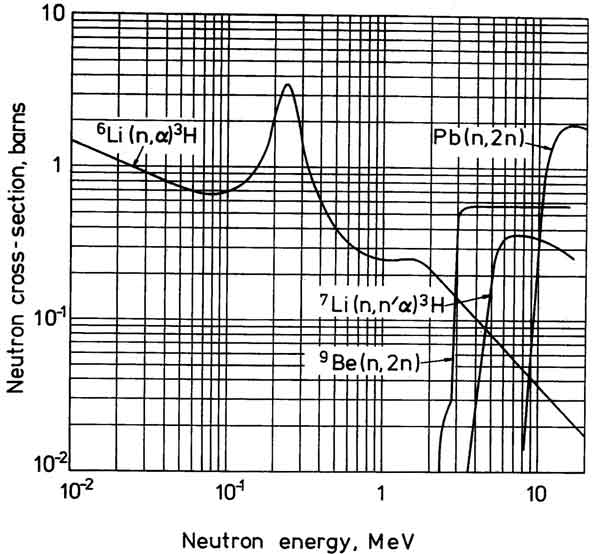
\includegraphics[width=\singleimagewidth]{chapters/figures/breeding_xsecs} 
	\caption{Cross-sections of various blanket materials. Note the threshold for the $^7$Li and neutron multiplying reactions.}
	\label{fig:li-xsects}
\end{figure}

Fortunately, lithium, like deuterium, is quite abundant on Earth. There is enough lithium accessible in the Earth's crust to generate tritium for 30 million years worth of DT reactions.\cite{Chen2011}. Thus lithium is an excellent candidate for generating the tritium necessary to self-sustain the fusion reaction in a power plant. Fusion reactor designs include so-called tritium breeding blankets which surround the plasma volume with lithium, however the form of lithium as it exists in the breeding blanket is a source of continued research.



At present there are two main concepts for tritium breeder designs: those containing liquid or solid lithium. Many of the functional requirements are similar between the two designs but their implementations are quite different. While much research has been -- and continues to be -- performed on the liquid breeder design (for examples, see Refs.~\cite{Hartmann1937,Hunt2006,Shercliff1953,Sommeria1982,Xv1937,Alfve1942}), the work of this dissertation focuses solely on the reference solid breeder design. In the next section, while introducing the breeding blanket, I will refer to the blanket almost exclusively as simply ``solid breeder'' though it should be understood that many of the generic features and requirements of the solid breeder are shared with its sister design, the liquid breeder.

\subsection{Breeding Blanket for Fusion Reactors}


\begin{figure}[ht]
	\centering
	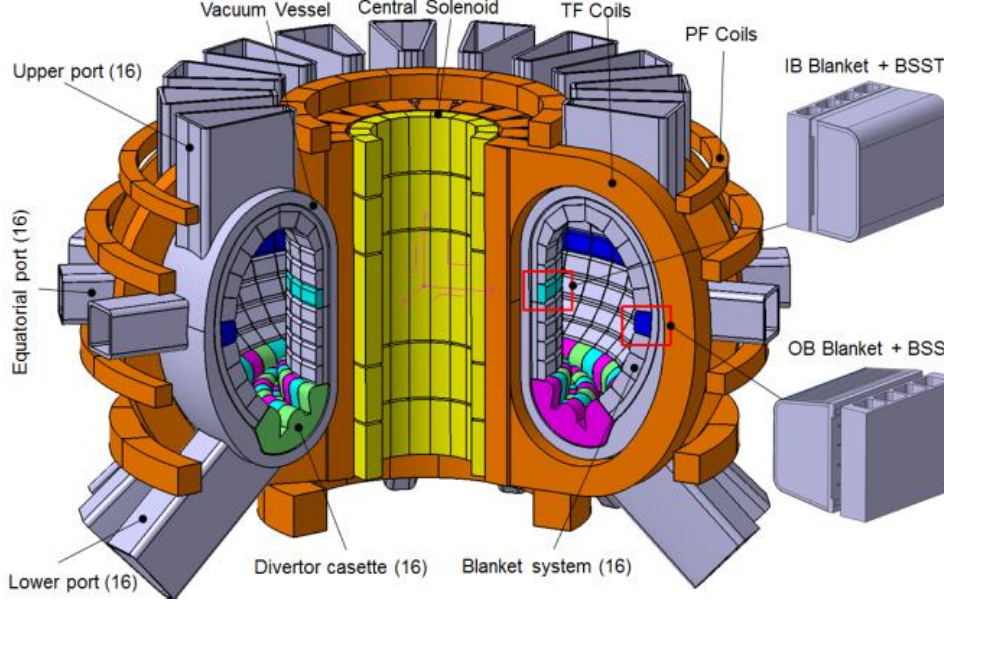
\includegraphics[width=1\textwidth]{chapters/figures/demo} 
	\caption{An example design of a DEMO reactor with solid breeder blankets shown as inboard (IB) and outboard (OB) blanket components.}
	\label{fig:demo}
\end{figure}

\begin{figure}[ht]
	\centering
	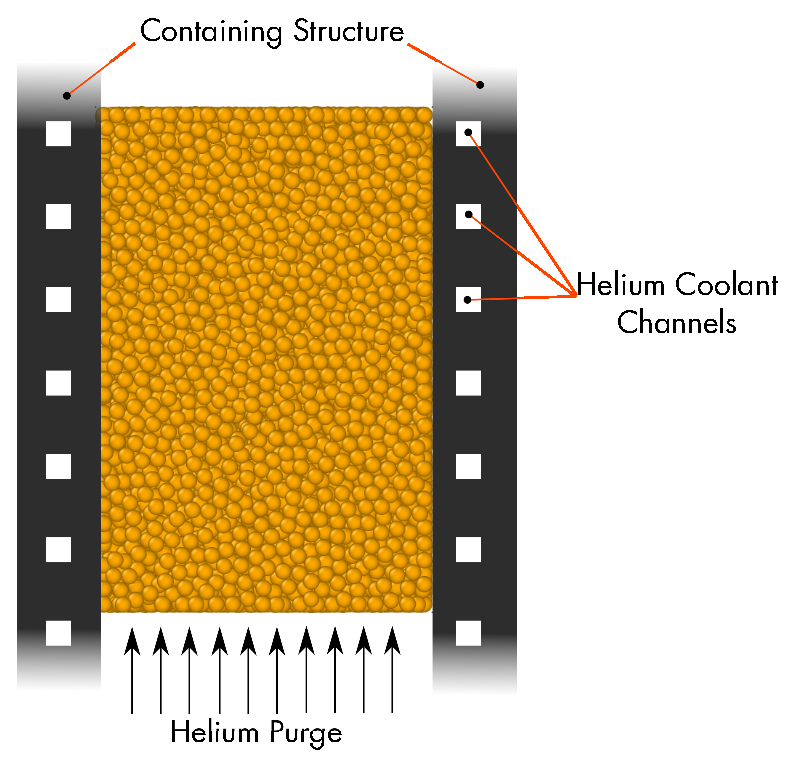
\includegraphics[width=\singleimagewidth]{chapters/figures/solid_breeder_sketch} 
	\caption{Sketch of a typical unit of a pebble bed tritium breeding zone. The pebble bed is cooled with contact to the containing structure.}
	\label{fig:solid-breeder-sketch}
\end{figure}

The breeder blanket is a critical piece of engineering technology upon which the success of a fusion power plant largely rests. The successful operation of a breeder will see the device capture the neutrons ejected from the fusion reaction to generate fuel for future reactions, act as shield to other sensitive equipment and personnel, and convert energy into extractable heat for electricity production. Figure~\ref{fig:demo} shows an example sketch of a demonstration (DEMO) fusion reactor and the relative location of the breeder blanket modules as they face the plasma in the torus of the tokamak. 

From the inception of the solid breeder concept in 1975 by Abdou\etal\cite{Abdou1975c}, designs have evolved significantly in response to requirements of operation in the harsh fusion environment. Currently, the reference solid breeder design incorporates packed beds of ceramic pebbles (spherical particles) that are filled into containment structures of volumes optimized for thermophysical and tritium responses. 

The pebble bed form has ultimately become the design of choice based on many of its attractive features. Many requirements of a solid breeder `material' (the volume of a pebble bed is often considered as a single fictitious material) are satisfied by the ceramic pebble bed. The small pebbles provide a sufficient surface-area to volume ratio; have good and customizable (via polydispersity) open-porosity to allow the helium purge gas to wind through and pick up any generated tritium from the solid; and the small size of the pebbles prevent any large thermal gradients from emerging across any single solid material object -- thus increasing the mechanical survivability of the ceramic. 

The representative pebble bed, as sketched in Fig.~\ref{fig:solid-breeder-sketch}, is shown to be contained by a low-activation steel which serves as both mechanical and thermal boundaries for the ensemble. The breeding blanket will experience high volumetric heating (resulting from secondary $\gamma$ rays and the kinetic energy of neutrons that are carrying away approximately 80\% of the fusion reaction) and temperatures will be allowed to increase to approximately 900~\celsius. The heat is conducted via inter-particle contacts between pebbles, contact with the structural material, and convection to the purge gas then transported to the structural material. A high pressure (approximately 8 MPa) helium coolant is then run through the structure. The coolant will heat to approximately 500~\celsius~before exiting the blanket, maintaining the steel below structural temperature limits. The heat carried away by the coolant ultimately works its way into an electricity-producing cycle. 

As the neutrons bombard the lithiated ceramic, tritium is produced internal to the pebbles. Tritium that transmutes from the lithium inside the pebble will diffuse slowly through the bulk until reaching a grain boundary. Tritium moves relatively quickly along the grain boundary until reaching a surface of open porosity where it may desorb into the passing purge gas.\cite{Federici1990} The low-pressure, low-speed purge gas is pumped through the pebble bed to extract the tritium generated and transport it out of the blanket for processing. 

The dual role of the breeding blanket to generate heat and tritium forces a specific operational temperature window for the ceramic pebble beds. The low end of the temperature window is governed by a minimum temperature for acceptable release rates of tritium from the ceramic to the purge gas; the value is generally set around 300~\celsius. Based on the current understanding of tritium release from the pebble, as grains grow during sintering of the ceramics the tritium release rate is expected to decrease beyond acceptable limits. Thus the upper limit of the temperature window is chosen to avoid sintering of the lithiated ceramic, giving the approximately 900~\celsius~limit mentioned previously. 

\begin{figure}
        \centering
        \begin{subfigure}[b]{\doubleimagewidth}
                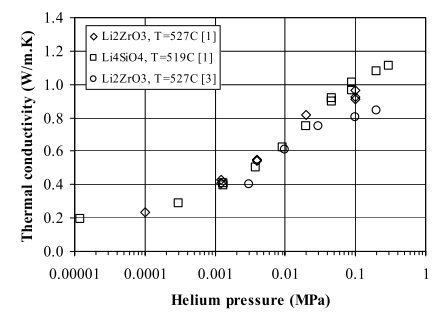
\includegraphics[width=\textwidth]{chapters/figures/keff-pressure}
                \caption{Effective conductivity of ceramic pebble beds is dependent on the pressure of the interstitial gas, a minimum of about $\keff = 1$~W/m-K in vacuum.}
                \label{fig:keff-pressure}
        \end{subfigure}%
        
          %add desired spacing between images, e. g. ~, \quad, \qquad, \hfill etc.
          %(or a blank line to force the subfigure onto a new line)
        \begin{subfigure}[b]{\doubleimagewidth 	}
                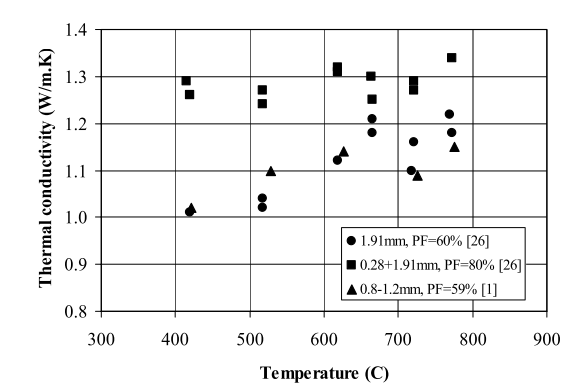
\includegraphics[width=\textwidth]{chapters/figures/lit-keff-exp}
                \caption{The effective conductivity of pebble beds is weakly dependent on external mechanical pressure and is always approximately $\keff = 1$~W/m-K in helium.}
                \label{fig:keff-lit}
        \end{subfigure}
        \caption{Effective conductivity of lithium ceramics. Results from Ref.~\cite{Abou-Sena2005}}\label{fig:keff}
\end{figure}

Many experiments have been run to measure the effective thermal conductivity of a volume of ceramic pebbles. In Figs.~\ref{fig:keff}, the effective conductivity is seen to be strongly affected by the interstitial gas but weakly affected by the mechanical loads on the bed. The main conclusions to bear in mind from Fig.~\ref{fig:keff} are that: 1) the interstitial gas is an important transporter of heat in the bed and 2) the effective thermal conductivity of the pebble bed is low and will limit the size of the ceramic pebble bed volume to satisfy the temperature window mentioned above.

% The size of breeder region is limited by the operational temperature window that must be held in spite of the the poor effective conductivity of packed beds of ceramic pebbles. The conductivity is experimentally shown to be a weak function of external pressure but can generally no greater than about \si{1 W/{mK}} -- for well-packed beds. Because the effective conductivity and packed bed-wall interface conductance is predominately a contact conduction, disruptions to the packing structure will have considerable impact on the heat transfer of the packed bed.

As nuclear energy is deposited into the poorly-conductive ceramic breeder material and the temperature climbs well above the containing structure, the pebbles will each individually begin to grow from thermal expansion. The containing structure will confine the thermal expansion of the lithium ceramic and therefore lead to large mechanical stresses at the points of contact of the individual pebbles in the packed bed. As a ceramic material, the pebbles are prone to brittle failure when the contact forces grow large. But the ceramic pebble beds must be able to survive the high temperature, high stress, and irradiated environment while providing a reliable amount of tritium to the fuel processing equipment.




 % the fusion reaction deposits   The nuclear heat generated in the pebble bed solid breeder will heat the ceramic pebbles to maximum temperatures of approximately 900~\celsius. The heat of the pebbles is transported through them via conduction through inter-particle contacts, conduction through the purge gas into neighboring particles, and ultimately through contact with the containing structure. The box structure surrounding the solid breeder will have high pressure (\si{8~MPa} in many current designs) 


\section{Motivation}\label{sec:motivation}

\begin{figure}[ht]
	\centering
	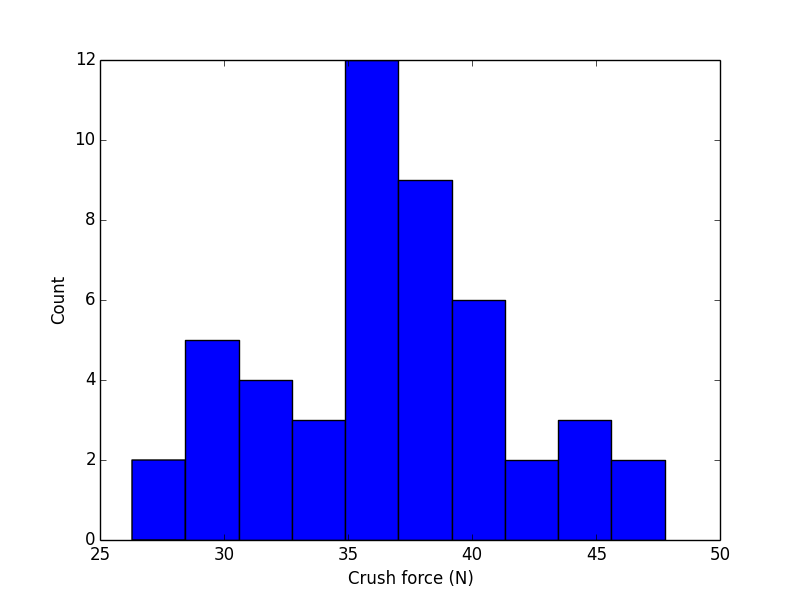
\includegraphics[width=\singleimagewidth]{chapters/figures/fmax} 
	\caption{Crush load distribution for a batch of $d_p = 1$~mm \lit pebbles.}
	\label{fig:fmax}
\end{figure}


Experiments on individual particles betray the brittle nature of ceramic pebbles and their propensity to break at relatively low individual contact forces. An example histogram of the crush loads of a batch of 1~mm \lit pebbles, as measured in our lab, is shown in Fig.~\ref{fig:fmax}. For these particular pebbles, the average crush load was less than 40 N. For some \lis pebbles, the average crush load is measured as low as 10 N. The relatively low force required to crush, coupled with the strong macroscopic loads predicted by the FEM models, brings into question the survivability of the pebbles and packing of the solid breeder.

If individual pebbles in the packed bed ensemble begin to crush, it may result in a number of negative effects on the bed. First, from Fig.~\ref{fig:keff-pressure}, we can see that a significant amount of heat (roughly 20\%) is transported through the bed purely via contact conductance between pebbles. In response to damaged pebbles, the bed will resettle from the imbalance of inter-particle and gravity forces. Any disruption in the contact network will have an impact on the heat paths internally and at the bed-wall interface. A bed with damaged pebbles could have significantly different effective thermophysical properties than those predicted for the original bed, potentially increasing the overall temperature of the bed past the acceptable temperature windows described in the previous section. Furthermore, the neutron absorption/shielding function of the solid breeder is dependent on an assumption of homogeneous distributions of pebbles in the breeding unit volume. Broken pebble fragments will settle, in time, in the direction of gravity and accumulate at the floor of the pebble bed, concurrently the entire bed may be resettling and a physical gap at the top of the pebble bed can form. This would result in undesirable quantities of neutrons streaming past the solid breeder volume. 

As the thermophysical properties evolve, global or local bed temperatures change and ultimately the tritium release characteristics of the bed deviate from any prediction one may have had from the initial packing of the ceramic pebble bed. The ceramic solid breeder must continue operating despite the harsh effects of existing in the fusion reactor. And it must continue operating without being replaced or actively maintained. Its important that the solid breeder not simply survive the thermal and mechanical demands of the reactor environment but continue to release predictable and acceptable amounts of tritium. 

In light of the short discussion above, it is apparent that a thorough study of pebble damage, including the loads on the pebble bed that will lead to broken pebbles as well as the pebble bed's thermophysical responses to broken pebbles, is critically needed for solid breeder design. Unfortunately, pebble bed experiments are inadequate for this need. The majority of measurements are only available for macroscopic properties (\textit{e.g.} uniaxial compression tests for stress-strain responses) or give only maximum measurements of individual pebble responses (\text{e.g.} pressure sensitive layers giving pebble pressures on a wall). The inability of physical experiments to reliably look into the transient inner structure of the pebble bed has driven past solid breeder researchers to employ pebble-scale models. Increasingly reliable and accurate models are crucial in the design of operational solid breeder blanket technologies. In this dissertation, I attempt to advance the field of solid breeder pebble-scale modeling with the introduction of new techniques and tools to incorporate the many facets of pebble damage in a solid breeder.

Briefly, I must consider why one would employ pebble-scale models versus those that are bed-scale. Afterall, the volume of a pebble in a tritium breeder is on the scale of 10$^{-9}$~m$^3$ while the typical container volume can be on the order of 10$^{-2}$~m$^3$\cite{Cho2008}.  Thus a single breeder volume will house upwards of $N = 10^7$ pebbles. Statistically then, it is reasonable to assume that continuum theory is applicable to the ensemble of pebbles. This assumption is the basis of development of finite element method (FEM) models for the breeder pebble beds. Constitutive equations are developed from experimental measurements of the macroscopic behavior of pebble beds which are fed into FEM models. The continuum assumption allows modeling the thermomechanical interaction of the entire pebble bed with the containing structure and coolant. The FEM models have been able to predict thermo-mechanical behavior with reasonable accuracy of some lab-scale experimental mock-ups of breeding units (A more thorough summary of the state of solid breeder modeling is given in \cref{sec:modeling-state}).\cite{DiMaio20081287,Zaccari20081282,Gan:2009vn} A notable result indicated by all the different FEM models is the indication that strong mechanical loads will arise throughout the pebble bed -- which will lead to many histrionic effects. But it is these very histrionic effects that FEM is, at present, incapable of modeling: pebble damage, resettling, and gap formation. The focus of this dissertation is on the histrionic effect of individual damaged pebbles and the morphological changes they induce in the pebble bed writ large. Thus I am compelled to consider the models at the scale of the individual pebbles.

\section{Scope of the Work}\label{sec:intro-scope-of-work}

In our group we identify the need to predict pebble damage in an ensemble, understand of the evolution of pebble bed morphology due to pebble damage, and analyze the impact of morphological changes on thermophysical and thermomechanical properties. To satisfy these needs, the work of this dissertation is to develop tools for modeling pebble interactions, predict pebble crushing based on the interactions, and monitor the macroscopic changes to temperatures in the bed in response to damaged pebbles. On the path of pebble-scale modeling development, I will:
\begin{enumerate}
	\item validate the Hertzian assumption for ceramic pebble interactions with single experiments on crushing pebbles,
	\item derive a criteria for pebble crushing in our numeric ensemble based on single pebble experiments,
	\item assess the impact of fragment size on packing resettling and other morphological features,
	\item calculate the evolving force network and its influence on the heat transport in the pebble bed.
\end{enumerate}

After implementing a sophisticated pebble-scale modeling tool, I will show the limitations of the micro-mechanical model when it comes to simulating the heat transfer of a ceramic pebble bed with a creeping helium purge gas. Thus I also implement some efficient bed-scale models of thermo-fluid flow coupled to/integrated with particle-scale mechanics. The steps toward achieving these models includes:
\begin{enumerate}
	\item adapting and employing two numerical schemes to study packed bed energy transfer with interstitial gas,
	\item analyze the reduction in $\keff$ due to broken pebbles,
	\item study the lumped-capacitance assumption (innate to the particle-scale modeling approach) in a packed bed with high Biot number with nuclear heating.
	\item address the overall impact of the helium purge gas on the thermal transport in a bed with evolving morphology,
\end{enumerate}

Finally, when the particle-scale model predicting and simulating pebble damage is coupled to thermo-fluid models of the helium purge through packed beds, I will use the numerical tools to judge the consequences of pebble damage on two ITER-relevant configurations of breeder volumes, applicable as guidance to solid breeder designers.



% The objective of this dissertation is to develop numerical models of ceramic pebble beds, based on first principles and experimental observations, to simulate the hysteritic evolution of pebble bed morphology and predict the subsequent changes to heat transport characteristics after thermally-induced damage to pebbles. The numerical tools are constructed in the following progression: 1. Transient DEM code of inter-particle interactions is employed to simulate packed bed restructuring in the wake of crushed pebbles in the ensemble -- and the effective thermal conductivity following the restructuring, 2. Transient, volume-averaged equations of Navier-Stokes and energy of the helium purge gas are coupled to the DEM model of pebbles to simulate conjugate heat transfer and the interstitial fluid influence on thermophysical properties after crushing events, 3) Complete simulations of the tortuous path of helium purge gas with lattice-Boltzmann models (based on the packing structure determined in DEM simulations) to expose flattened temperature profiles due to laminar mixing in the pebble bed. 

In summary, understanding the evolution of pebble bed morphology and its impact on thermophysical properties is critical for solid breeder designers. The understanding allows for temperature control of breeder pebble beds over the operational lifetime of the blanket which is crucial to the function of the solid breeder for tritium and energy generation. The tools I develop in the course of this dissertation are a necessary step toward realization of this understanding. 

One last note: there are other long-term effects expected in the materials experiencing prolonged exposure to cycling irradiation, heat, and stress that have not been discussed here. These loads can lead to thermal ratcheting, irradiation swelling, sintering, or thermally-induced creep which also lead to evolutions in thermophysical properties -- even in the absence of cracked pebbles. These phenomena need to be addressed in time but are, however, beyond the scope of this dissertation. 
% we aim to provide designers of packed beds with tools to understand how packing states may evolve from time-dependent phenomena (e.g. sintering, creep, pebble cracking, etc.). These phenomena may, for instance: decrease the effective thermal conductivity which will raise bed temperatures beyond initial predictions, produce isolated pebbles which will sinter and potentially decrease tritium release rates, or even form gaps between pebble beds and containing structures leading to divergence from properties of the initial packing of the bed.

% The objective of this work fits into the broader mission of our research group in the UCLA Fusion Science and Technology Center to develop and apply complete numerical models of ceramic pebble bed solid breeder modules. Any complete numerical model for a pebble bed would require the interaction of many sub-models or sub-functions operating at disparate scales. To demonstrate, a possible top-level algorithm could proceed in the following way: To begin, one must have knowledge of the interaction of the pebble bed with the containing structure as they exist in a fusion environment. The interactions are generally analyzed via the finite element method to find internal stresses and temperature fields of the entirety of the pebble bed and surrounding container. After the internal fields are mapped into the bed, one would use the discrete element method (DEM) to interpret the macroscopic stress fields into the inter-particle forces. With the inter-particle forces and total absorbed thermal energy calculated, a prediction of the initiation and evolution of morphological changes (i.e. crushed pebbles, sintering, creep, etc.) to each computational volume. Following this, DEM would calculate new effective properties as a result of the morphological changes to the pebble bed region. Finally, the updated bed properties would feed back into the FEM formulation to update calculations in the macroscopic stress fields. While a suite of integrated numerical tools that follows this example algorithm is the ultimate goal of our group, the work of this dissertation is focused entirely on the development of pebble-scale simulations that are predominately in the realm of the discrete element method.

% In the following subs-sections, we briefly outline the studies fitting into the scope of this dissertation. 

% \subsection*{Discrete Element Method Study on the Evolution of thermo-mechanics of a Pebble Bed Experiencing Pebble Damage}
% In the first study of \cref{sec:dem-studies}, we analyze the effective thermal conductivity of a pebble bed assuming different fractions of pebbles in the ensemble are completely crushed. The focus of this study is to 1) determine the extent of change, in aggregate, to ensemble properties due to individual pebble crushing, 2) relate the changes in effective conductivity to quantifiable pebble-scale properties (e.g. contact force, coordination number, etc.), 3) use the results to create guidelines for designers to anticipate acceptable limits of pebble loss from a thermal management point of view. For the DEM tools used in this study, the only mode of heat transfer considered is conduction between the solid particles. 


% \subsection*{Coupling DEM Models of Ceramic Breeder Pebble Beds to Thermofluid Models of Helium Purge Gas Using Volume-averaged CFD}
% In a fusion breeder, the helium purge gas winding through the interstitial gaps of the pebbles has a substantial contribution to overall heat transfer.\cite{Reimann:2002mi,Abou-Sena2005} The model of \cref{sec:dem-studies} is improved to include the flowing interstitial gas. In \cref{sec:cfd-dem-studies}, we continue to employ our DEM tools to provide particle-scale information such as contact force, but couple the pebbles to a volume-averaged computational fluid dynamics (CFD) code for the conjugate heat transfer simulation. The coupled CFD-DEM model is used to again simulate the heat transfer in packed beds of ceramic spheres that experience pebble crushing -- but now with a focus on highlighting the impact of a flowing interstitial helium purge gas when pebbles are crushed.


% \subsection*{Lattice-Boltzmann Method Integrating DEM Packing Structures to Study Laminar Mixing}
% The models to account for helium purge gas employed in the studies of \cref{sec:cfd-dem-studies,sec:applied-studies} assume effective drag or heat transfer coefficients for pebbles in a computational volume and then include the pebble influence through effective source/sink terms in the momentum and energy equations. The volume-averaged approach allows for simpler meshing of the fluid volume while still retaining much of the physical realism of the system. Complete models of the conjugate heat transfer of both the fluid moving through the tortuous interstitial gaps pebble beds pressing each other with small contact areas are intractable with current computational hardware and finite-element modeling techniques. To overcome deficiencies in computational power, in \cref{sec:modeling-lbm}, we apply a relatively new technique wherein a lattice-Boltzmann algorithm solves for complete flow fields and conjugate heat transfer of helium winding through a packed bed. The lattice-Boltzmann method (LBM) is a non-traditional fluid simulation technique that allows us to resolve pebble/pore-scale momentum and energy transfer. The LBM approach is applied to the same pebble beds analyzed in \cref{sec:cfd-dem-studies} to provide comparison between the two modeling techniques. Furthermore the LBM model, accounting for the complex helium purge gas pathways, provides more insight to the influence of helium on the heat transfer in the heat transfer of packed beds.





% \subsection*{Modeling Tools to Study Coolant Designs of ITER Solid Breeder Module Volumes}
% In the study of \cref{sec:applied-studies}, we apply our coupled helium-pebble computational tools to the analysis of ITER-relevant solid breeder geometries. In this study we consider the combined effects of pebble crushing, packing restructuring due to both gravity and the unbalanced force network in the pebble bed, and convection from helium purge gas on temperature profiles in solid breeders for different breeding configurations. Heat transfer out of the pebble bed relies on maintaining good pebble-pebble and pebble-wall contact. However, physical contact is interrupted to different degrees when a pebble bed responds to various amounts of individual crushed pebbles. Furthermore, the restructuring of the pebble bed after a pebble crushing event is, in part, dependent on gravity forces acting upon each pebble in the ensemble. We investigate two representative pebble bed configurations where heat is removed from the bed via inter-particle conduction, convection of purge gas, and contact between the pebble bed and its container. In the first, the coolant containing structural walls (heat transfer walls) are oriented parallel to the gravity vector. In the second configuration, the heat transfer walls are perpendicular to the direction of gravity. To simulate a crushed pebble, we replace the pebble with many smaller, non-cohesive elements while maintaining mass-conservation between the original solid pebble and crushed fragments. The fragments are then free to resettle into interstitial gaps and the rest of the bed resettles as determined by forces from gravity, contact of neighboring particles, and even the small influence of the moving purge gas. The thermo-fluid interaction with the helium purge gas will be included with volume-averaged Navier-Stokes and energy equations. The representative solid breeder volumes will be compared with respect to their temperature peaks and profiles and how those temperatures vary as a function of the percentage of crushed pebbles in the ensemble. The results can be used to optimize solid breeder pebble bed designs through the choice of breeding zone orientation relative to the gravity vector.



% \chapter{Dissertation Outline}
% The path toward the modeling efforts outlined for the scope of this work is not a clear, straight line. To accomplish the goals set forth -- attempting to discuss them in the most clear and accurate way possible -- this dissertation is broken up into five major parts following their logical partitions. This section, Part I, provides the introduction and motivation behind the work. In Part II, (containing Chapters: \cref{sec:hertz-theory,sec:modeling-state,sec:survey-packed-beds}) we survey the state of the art in analysis of ceramic pebble beds, contact mechanics, and modeling thermal and mechanical interactions of particles in packed beds and fluids moving interstitially.  In Part III, (containing Chapters: \cref{sec:modeling-dem,sec:modeling-cfd-dem,sec:modeling-lbm}) we outline the numerical methodology and development of modeling tools we shall use in the study and analysis of pebble beds and their evolving morphology due to external loads. We compartmentalize the numerical tools into three parts, namely: the discrete element method (DEM), coupled computational fluid dynamics and the discrete element method (CFD-DEM), and a lattice-Boltzmann method (LBM) we integrate with DEM. The development of the tools is assisted with theoretically- and experimentally-based studies on individual pebbles in an ensemble. The newly developed enhancements to the numerical tools are studied before their inclusion in the toolkits. We work through the results of the promised studies in Part IV (\cref{sec:cfd-dem-studies,sec:dem-studies,sec:lbm-studies,sec:applied-studies}). Finally, in Part V, we discuss the next steps to be taken that we identify as critical next steps -- but beyond the scope of this dissertation -- for the modeling tools. In addition, other research avenues that have been opened by the tools introduced and their potential impact are discussed here.
% \input{chapters/background-discussion.tex}


% Content
%%%%%%%%%%%%%%%%%%%%%%%%%%%%%%%%%%%%

\chapter{Pebble Interaction Analysis: Theory} \label{sec:analysis-theory}


This chapter will walk through the analysis first performed by Heinrich Hertz in 1880 of idealized interacting spherical objects to represent our ceramic pebbles. We will begin with mechanical interactions of purely elastic spheres and then use the results to develop a theory for conductive heat transfer between the pebbles. Finally, Hertz's theory will also be used to analyze pebble interaction with flat plattens in our test stand used to measure crush force. A relationship is developed allowing us to translate from experimental results to pebble bed ensembles.

%%%%%%%%%%%%%%%%%%%%%%%%%%%%%%%%%%%

% Included sections
\section{Hertz theory for normal contact of spheres}\label{sec:hertz-contact}
[DRAW SOME COORDINATE DIAGRAMS TO SHOW HOW Z R AND X-Y WHATEVER ARE ACTUALLY RELATED AND CAN BE VISUALIZED]
We consider two non-conforming solids approaching and then contacting under load. We only wish to analyze the contact of spheres (of differeng radii), so we are able define the surface curvature of the two contacting bodies as

\begin{align}
z_1 &= \frac{1}{2R_1}r^2 \\
z_2 &= \frac{1}{2R_2}r^2
\end{align}

respectively. The radius, laying in the $x-y$ plane is related to cartesian coordinates as $r^2 = x^2 + y^2$. Before the surfaces are in contact, each point on the two surfaces are separated by a distance $h(r)$,

\begin{align}\label{eq:separationh}
h &= z_1 - z_2 \nonumber \\
h & = \left(\frac{1}{R_1} + \frac{1}{R_2}\right)\frac{r^2}{2} 
\end{align}

We define the relative radius of curvature as

\begin{equation}\label{eq:relativeRadius}
\frac{1}{R^*} = \frac{1}{R_1} + \frac{1}{R_2}
\end{equation}

and then the separation is simply $h = (1/2R^*)r^2$.

\begin{figure}[ht!]
	\begin{center}
	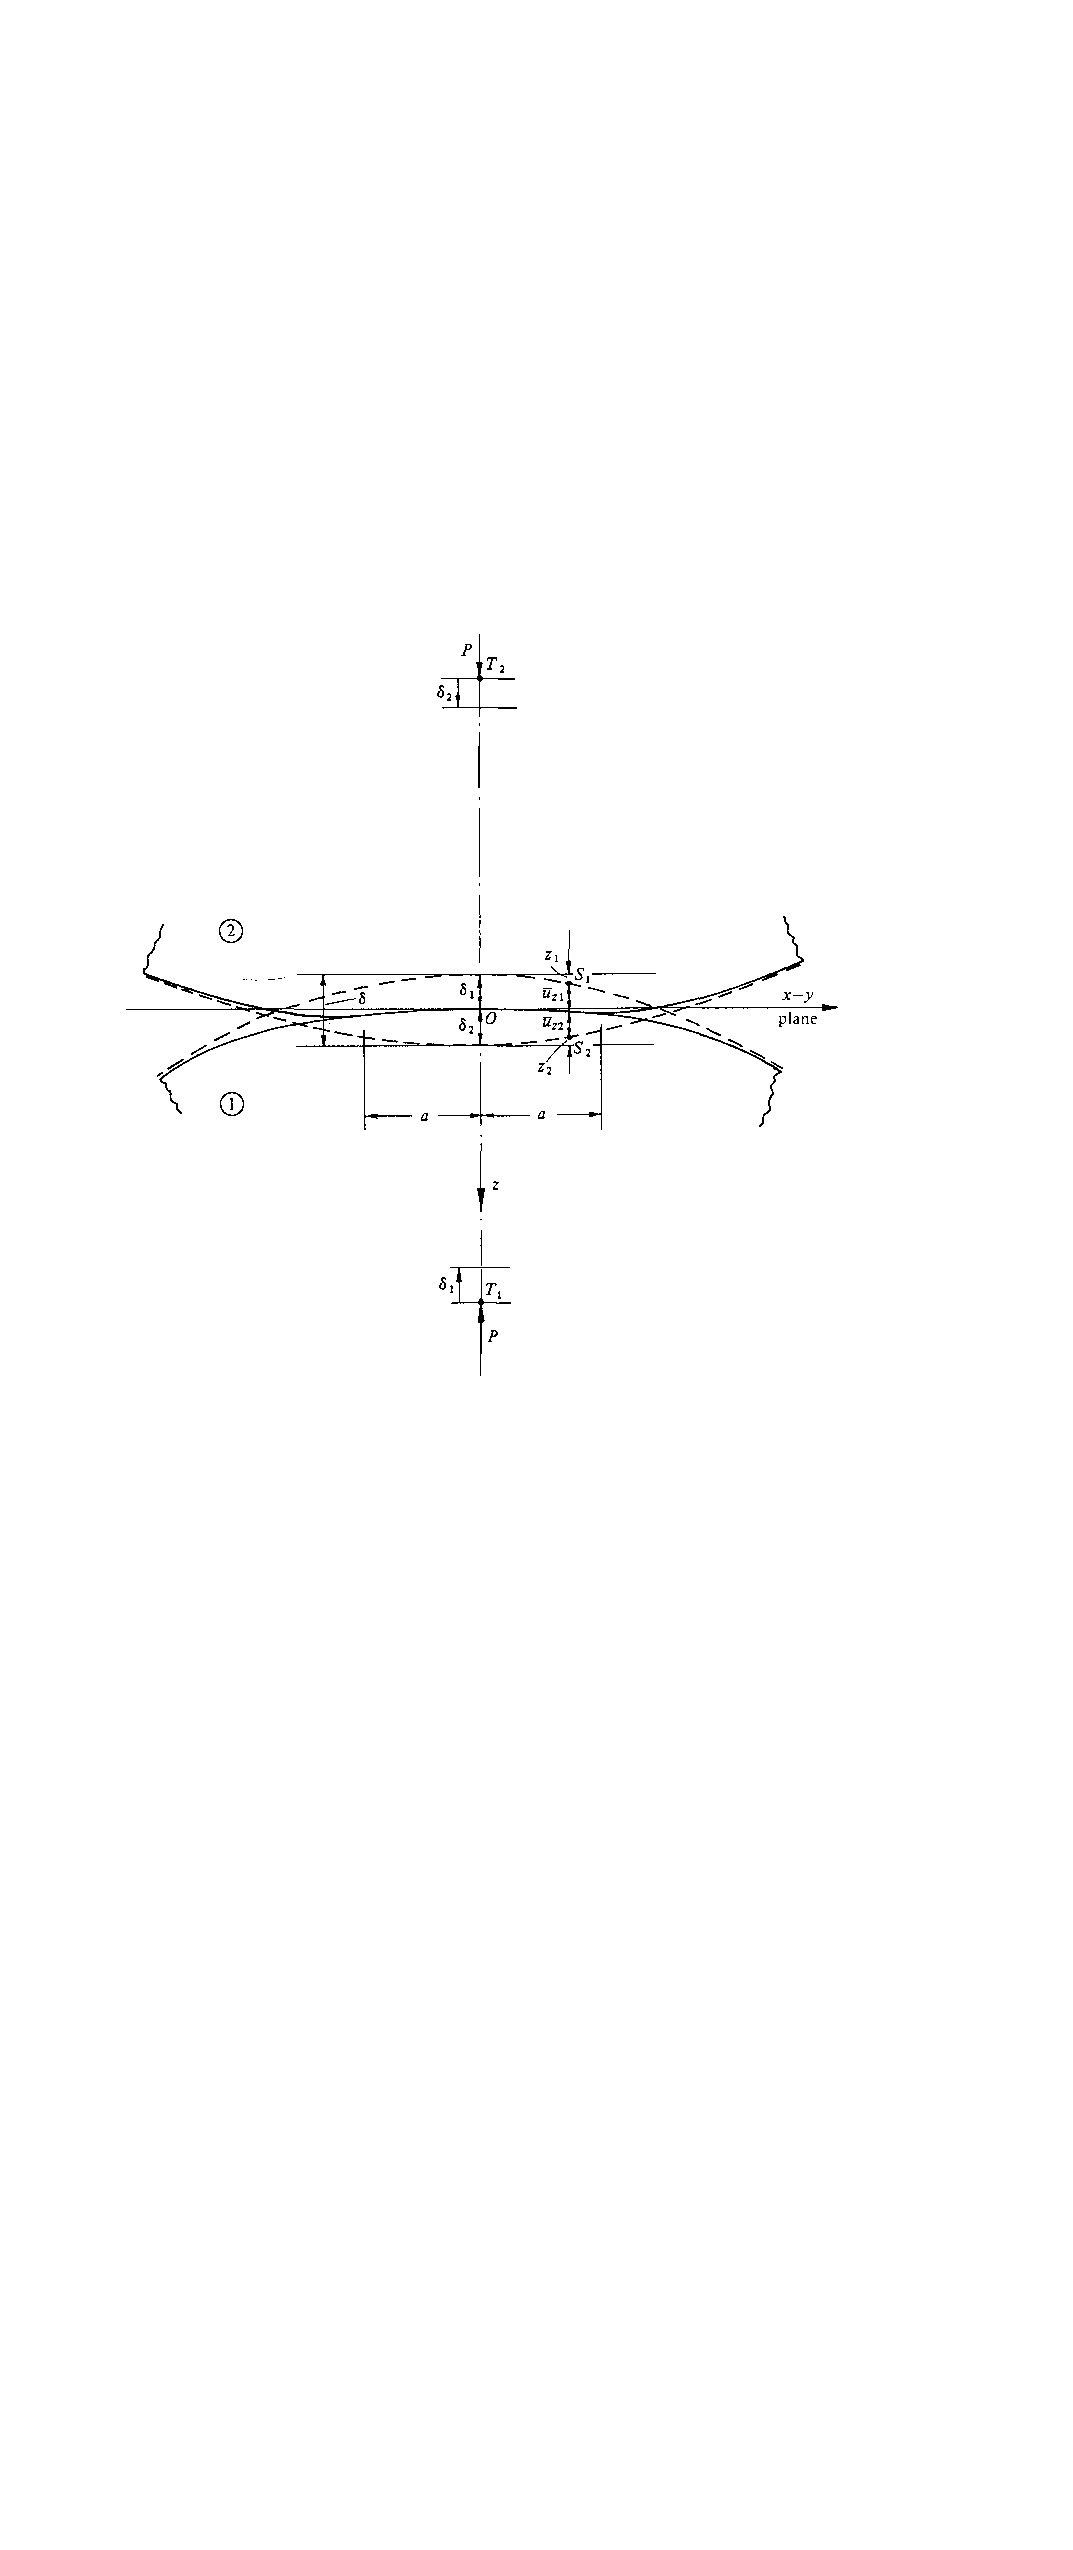
\includegraphics[width=0.95\textwidth]{chapters/figures/hertzGeometry}
	\caption{default}
	\label{fig:hertzgeometry}
	\end{center}
\end{figure}

We allow the two surfaces to approach, and then, under an external load $F$, contact. The cross-section of these bodies after contact are shown in Fig.~\ref{fig:hertzgeometry}. If we first imagine that the two surfaces do not interact and their surfaces pass through each other unimpeded, their surfaces would be overalapped to a distance $\delta$. In such a case, we examine two points deep within the bodies, along the axis of contact, calling them $T_{1}$ and $T_2$. These points will have moved $\delta_1$ and $\delta_2$, respectively. The total overlap is obviously related to these displacements by $\delta = \delta_1 + \delta_2$. 

However, under actual contact, the two surfaces are going to deform as the load $F$ presses them into contact. So now we consider two points on the surfaces, such as $S_1$ and $S_2$. Before contact, these two points are initially are separated by a distance $h$ (from Eq.~\ref{eq:separationh}), then displace by $\bar{u}_{z1}$ and $\bar{u}_{z2}$ due to contact pressure. 

If the points $S_1$ and $S_2$ are inside of the contact region under load, these distances are related by

\begin{equation}
	\bar{u}_{z1} + \bar{u}_{z2} + h = \delta
\end{equation}

Then using Eq.~\ref{eq:separationh}, we have an expression for the elastic displacements:

\begin{equation}\label{eq:hertzdisplacements}
	\bar{u}_{z1} + \bar{u}_{z2} = \delta - \frac{1}{2R^*} \, r^2
\end{equation}

Alternatively, if after deformation the points $S_1$ and $S_2$ are outside of the contact region, this is simply

\begin{equation}\label{eq:hertz-disp-2}
	\bar{u}_{z1} + \bar{u}_{z2} > \delta - \frac{1}{2R^*} \, r^2
\end{equation}

It now is necessary to find a pressure distribution that satisfies these boundary conditions of displacement. Heinrich Hertz first formulated the expressions of Eqs.~\ref{eq:hertzdisplacements,eq:hertz-disp-2} in 1882. The power of his solution is borne out by the continuous use of his theory since that time. Hertz simplified the problem by regarding each body as an elastic half-space upon which the load is applied over a small, elliptical region (the contact area). This simplification allows for treatment of the highly concentrated stresses near the region of contact without consideration of either the general response of stresses in the bulk of the body or the manner in which they are supporting the load. This assumption is justifiable if the dimensions of each body as well as the relative radii of curvature are very large compared to the contact area. These assumptions are sufficient to proceed with the analysis, but the curious are pointed to an excellent discussion and background of Hertz's theory as given in KE Johnson's textbook~\cite{Johnson1985}.

For solids of revolution, a distribution of pressure to satisfy the displacements of Eq.~\ref{eq:hertzdisplacements,eq:hertz-disp-2} is proposed by Hertz as

\begin{equation}
	p = p_0 \left[1-\left(\frac{r}{a}\right)^2\right]^{1/2}
\end{equation}

where $a$ is the radius of the contact area.

The total load, $F$ is found from the pressure distribution as

\begin{align}\label{eq:hertzforcewithpressure}
	F &= \int_0^a \! p(r) 2\pi r\, \mathrm{d}r\\
	F & = \frac{2}{3} p_0 \pi a^2
\end{align}

From the distributed load over the circular region, stresses and deflections are found from superposition of point loads. The pressure is integrated (see Ref.~\cite{Johnson1985}) to find the normal displacement for either solid body as

\begin{equation}
	\bar{u}_z = \frac{1-\nu^2}{E}\frac{\pi p_0}{4a}\left(2a^2 - r^2\right)
\end{equation}

This is applied to both bodies and plugged into Eq.~\ref{eq:hertzdisplacements} to yield

\begin{equation}\label{eq:pressindisplacement}
	\frac{\pi p_0}{4aE^*}\left(2a^2 - r^2\right) = \delta - \left(\frac{1}{2R^*}\right)\, r^2
\end{equation}

where we have introduced the now-common term of pair Young's modulus,

\begin{equation}
	\frac{1}{E^*} = \frac{1-\nu_1^2}{E_1} + \frac{1-\nu_2^2}{E_2}
\end{equation}

for simplification.

With the solution of Eq.~\ref{eq:pressindisplacement}, if we consider $r = a$ and $\delta(a) = 0$, we find the radius of the contact circle is

\begin{equation}
	a = \frac{\pi p_0 R^*}{2E^*}
\end{equation}

and when $r= 0$, we find the overlap as

\begin{equation}
	\delta = \frac{\pi a p_0}{2E^*}
\end{equation}

and alternatively we find the pressure as a function of overlap

\begin{equation}
	p_0 = \frac{2E^*\delta}{\pi a}
\end{equation}

The radius, overlap, and pressure relations are inserted into Eq.~\ref{eq:hertzforcewithpressure} to find the force (from now on referred to as the Hertz force) as a function of overlap, relative radius, and pair Young's modulus,

\begin{equation}\label{eq:hertz-force}
	F = \frac{4}{3}E^* \sqrt{R^*} \, \delta^{3/2}
\end{equation}

Equation~\ref{eq:hertz-force} defines the normal contact forces between any two contacting, elastic spheres. This extremely important result acts as the basis of all discrete element method codes since the concept was first introduced for granular materials by Cundall \& Strack in 1979\cite{Cundall1979}. To differentiate the force from other terms to be derived later, we specificy it as the normal force between sphere $i$ and sphere $j$ as

\begin{equation}\label{eq:hertz-normal-force}
	F_{n,ij} = \frac{4}{3}E_{ij}^* \sqrt{R_{ij}^*} \, \delta_{ij}^{3/2}
\end{equation}









%%%%%%%%%%%%%%%%%%%%%%%%%%%%%%%%%%%%%%%%%%%
\chapter{Pressure drop across packed beds} \label{ch:modeling-pressure-drop}
%%%%%%%%%%%%%%%%%%%%%%%%%%%%%%%%%%%%%%%%%%


%%%%%%%%%%%%%%%%%%%%%%%%%%%%%%%%%%%%%%%%%%
%\input{}
%%%%%%%%%%%%%%%%%%%%%%%%%%%%%%%%%%%%%%%%%%
%%%%%%%%%%%%%%%%%%%%%%%%%%%%%%%%%%%%%%%%%%
\chapter{Heat transfer in packed beds} \label{ch:modeling-heat-transfer}
%%%%%%%%%%%%%%%%%%%%%%%%%%%%%%%%%%%%%%%%%%
This section covers a discussion of different modes of heat transfer experienced by a pebble in a packed bed. The main modes are conduction to neighbors and convection.

%%%%%%%%%%%%%%%%%%%%%%%%%%%%%%%%%%%%%%%%%%
\section{Single particle heat transfer}

\begin{figure}[t]
	\centering
	\caption{Each ceramic pebble in a fusion reactor will experience multiple modes of heat transfer.}
	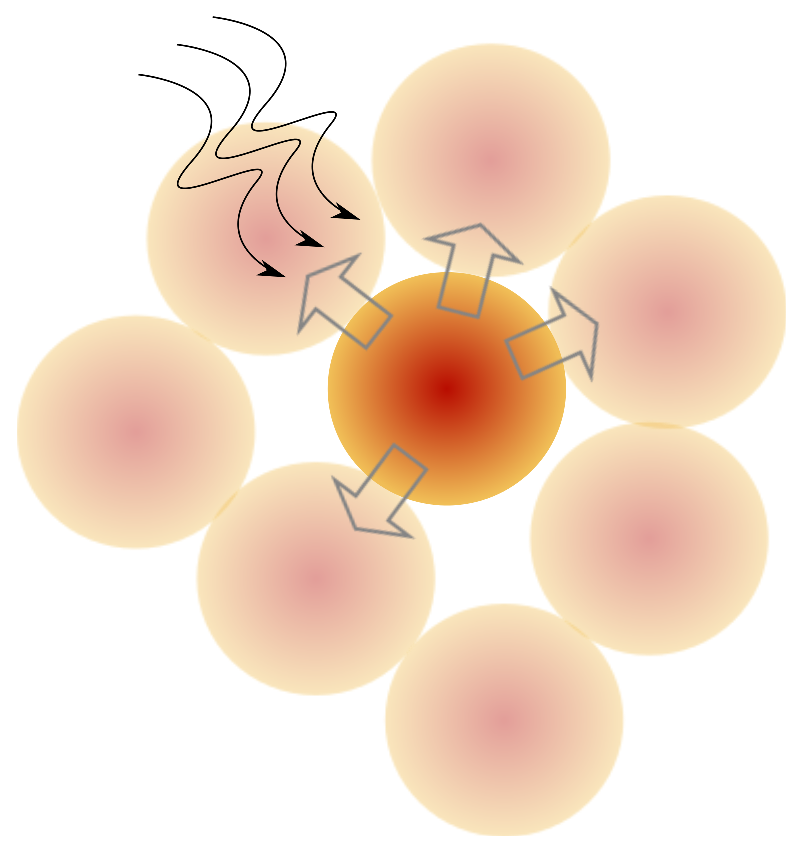
\includegraphics[width=0.75\textwidth]{chapters/figures/pebble-complete-heat-transfer}\label{fig:peb-comp-ht}
\end{figure}

Shown in Fig.~\ref{fig:peb-comp-ht} are all the modes of energy transfer on a pebble inside the fusion reactor. There is:

\begin{enumerate}
\item energy generated internal to the pebble caused by nuclear heating,
\item conduction internally of the solid material to the surface of the pebble, 
\item conduction between neighboring pebbles at their areas of contact, 
\item radiation between neighboring solids, and 
\item convective heat transfer with the interstitial helium gas (which includes energy carried far downstream or redeposited to neighboring pebbles).
\end{enumerate}









\subsection{Nuclear heating}

Nuclear deposition of energy is handled in a straightforward manner in the DEM computations with a simple source term on the energy balance equation. 












\subsection{Conduction through the solid}\label{sec:ht-pebble-conduction}

Before considering the heat equation in a sphere, it is instructive to first consider the simpler problem of a one-dimensional slab with volumetric heat generation, $q_g'''$ and convective cooling at the surfaces. The geometry is shown in Fig.~\ref{}.

Assuming we can find the Nusselt number for the convective cooling, we write the heat flux from the surface to the fluid as

\begin{equation}
	q_s'' = h(T_s - T_f)	
\end{equation}

where $T_f$ is the bulk fluid temperature and $T_s$ is the surface temperature. At steady-state the amount of heat moved across the fluid-surface interface must necessarily be equal to the total amount of heat generated into the slab. Therefore,

\begin{equation}
	q_w'' = q_g'''L = h(T_f-T_s)
\end{equation}

where $L$ is the half-width of the slab. For the sake of discussion, we re-write the above in terms of the temperature delta from surface to fluid in terms of nuclear heating,

\begin{equation}\label{eq:fluid-delta}
	T_f-T_s = \frac{q_g'''L}{h}
\end{equation}

Inside the slab, at steady-state the energy equation is simply a balance of heat conduction and nuclear generation. 

\begin{equation}\label{eq:nuclear-heating-slab-ode}
	0 = k\frac{\mathrm{d}^2T}{\mathrm{d}x^2} + q_g'''
\end{equation}

The boundary conditions are symmetry about the centerline and known surface temperature

\begin{align}
	q_{L=0} &= 0 \\
	T(L) &= T_s
\end{align}

The ODE of Eq.\ref{eq:nuclear-heating-slab-ode} is solved with simple separation and integration. When the boundary conditions are applied we have

\begin{equation}
	T(x) = \frac{q_g''' L^2}{2k}\left(1-\frac{x^2}{L^2}\right) + T_s
\end{equation}

We can find the temperature at the centerline of the slab, $x = 0$ as

\begin{equation}
	T_{cl} = \frac{q_g''' L^2}{2k} + T_s
\end{equation}

Or,

\begin{equation}\label{eq:centerline-delta}
	T_{cl} - T_s = \frac{q_g''' L^2}{2k}
\end{equation}

From Eqs.~\ref{eq:fluid-delta} and~\ref{eq:centerline-delta}, we see that the temperature differences between the surface and the fluid or the centerline and the surface are dictated by the heat generation rate relative to the speed at which that heat can be transported, via convection or conduction, respectively.

We will divide Eq.~\ref{eq:centerline-delta} by Eq.~\ref{eq:fluid-delta},

\begin{equation}\label{eq:biot-derivation}
	\frac{T_{cl} - T_s}{T_f-T_s} = \frac{1}{2}\frac{hL}{k}
\end{equation}

Careful observation of this equation can tell us much about the relative importance of the different modes of heat transfer to/from the surface. If the thermal transport away from the surface occurs at a much slower pace than thermal transport of energy through the solid to the surface, then the change in temperature across the solid $T_{cl}-T_{s}$ will be small compared to the change in temperature from the interface of solid to the bulkd fluid temperature, $T_{s}-T_f$. If the temperature across the solid is negligibly small in comparison to the surface-fluid difference, we are safe in the assumption that the solid is isothermal.

The group of terms on the right-hand-side of Eq.~\ref{eq:biot-derivation} is recognized as the Biot number,

\begin{equation}\label{eq:biot-number}
	\Bi=\frac{hL}{k}=\frac{R_{cond}}{R_{conv}}
\end{equation}

whose value is used to quantify the importance of internal conduction in the analysis of the solid interacting with convective heat transfer. If $\Bi<<1$, it is safely assumed that there is no temperature gradient in the solid material. A conclusion that will prove helpful in later analysis.

It is interesting to note that in this derivation of Biot number, we had considered nuclear heating as the source for temperature gradients across the pebble yet the rate of nuclear heating still does not appear in the Biot number. This implies that traditional assumptions of the validity of the lumped capacitance method hold even when dealing with a heat generation term in our energy balance.





\subsubsection{Large Biot number}

As we saw from the discussion of Eq.~\ref{eq:biot-number}, when the Biot number is small we can safely neglect temperature gradients through the solid we are analzying. However, when dealing with materials with low conductivity, i.e. larger $\Bi$, this assumption of negligible temperature gradient becomes decreasingly valid.  When dealing with spheres, there are slighty different accepted definitions of the Biot Number.  Some suggest that $\Bi=hd_p/6k$ is acceptable\cite{incropera:245}, where $d_p$ is the diameter of the particle.  However many use the more conservative definition of $\Bi=hd_p/2k$\cite{incropera:245,jeffreson409}.  For consistency and conservatism, we will proceed here with the latter definition.  

Considering now material and geometric properties relevant to our ceramic pebble beds, we will see that we may need to consider the effects of a larger $\Bi$ for our pebbles. The helium purge gas moving through the packed beds is not specifically intended to act as a heat transfer agent and moves along at a creeping flow rate. For a first approximation we will therefore assume as a lower limit the Nusselt number is $\Nu = 2$ (the value for a sphere in quiescent fluid). From the requirement that $\Bi \ll 1$, we have

\begin{equation}
	2 \frac{k_f}{k_s} \ll 1
\end{equation}

The conductivity of helium over the temperature range of 300 to 800 $^\circ$C is approximately 0.3 \si{W/m-K}. The solid conductivity of \lit and \lis are approximately 2 \si{W/m-K}. Because of the low conductivity of our solid, the Biot assumption is barely valid, $0.3 < 1$. 


































[Go back through Batchelor and O'Brien~\cite{Batchelor1977} paper]

\begin{equation}
	\frac{ k_s }{ k_f } \frac{a}{R^*} = \lambda
\end{equation}

Similar to the lumped capacitance assumptions, if $\lambda \gg 1$, the solid is approximately is isothermal. The second group on the left-hand side of this condition we remember from the assumptions of Hertz theory, where we require $\frac{a}{R^*} \ll 1^*$. Therefore to satisfy the condition of $\lambda \gg 1$, we require very large conductivity ratios of solid to fluid, $\frac{k_s}{k_f} \gg 1$. Alternatively this is satisfied by definition if the solids exist in vacuum.

Assuming that we satisfy the condition of isothermal solids, we address the conduction between solids in their small regions of contact.

[more details]










\subsection{Particle-particle conduction}

Handling the heat transfer between contacting particles has been investigated extensively by researchers in a number of fields\cite{Zhou2009,Zhang2011,Wu2011,Vargas2001,Li2000,Chaudhuri2006}. The amount of energy per time that can be transported per difference in temperature between pebble $i$ and $j$ as a conductance $h_{ij}$. Defined as

\begin{equation}\label{eq:pebble-conductance}
	\frac{h_{ij}}{k^*}= 2\left[\frac{3F_nR^*}{4E^*}\right]^{1/3}
\end{equation}

$k^*= 2k_ik_j/(k_i+k_j)$ is the effective solid conductivity of the two particles, and $F_n$ is the magnitude of the normal force between particles $i$ and $j$ as calculated by Eq.~\ref{eq:hertzForce}. Therefore, if we consider particles at temperatures $T_i$ and $T_j$ in contact, they will transfer heat at a rate of

\begin{equation}
	Q_{ij} = h_{ij}(T_i - T_j)
\end{equation} 











\subsection{Convection}











\subsection{Particle-particle radiation}
\subsection{Inter-particle heat conduction}\label{sec:ht-pebble-conduction}

When two particles come into contact, energy is transmitted through their region of contact. For this discussion, we assume the particles are spherical, elastic, in vacuum, and we neglect radiation transfer between them. If the two particles are at temperatures $T_i$ and $T_j$ we can quantify the amount of energy transferred between them with a commonly used practice of a contact conductance, $H_c$:
\begin{equation}\label{eq:pebble-conduction-heat-transfer}
	Q_{ij} = H_{c}(T_i - T_j)
\end{equation}

The subscripts are omitted for clarity, but obviously there is a unique $H_c$ per pair of contacting particles. We note that the heat conductance, unlike standard heat transfer coefficients, has units of \si{W/K}.

Batchelor and O'Brien\cite{Batchelor1977} developed a formulation of similar form and then made the brilliant observation that the temperature fields in the near-region of contacting spheres are analogous to the velocity potential of an incompressible, irrotational fluid passing from from one reservoir to another through a circular hole in a planar wall separating the two reservoirs. With the analogy, they could make use of the fluid flow solution to write the total flux across the circle of contact just as Eq.~\ref{eq:pebble-conduction-heat-transfer} with the heat conductance as

\begin{equation}\label{eq:batchelor-pebble-conductance}
	H_c = 2k_ra
\end{equation}

where $k_r$ is the conductivity of the contacting solids and $a$ is the radius of contact. In \cref{sec:hertz-theory}, with Hertz theory we found the contact radius in terms of the contact pressure. Here, we give the radius in terms of the compression force acting on the bodies,

\begin{equation}
	a =  \left(\frac{3}{4}\frac{R^*}{E^*}\right)^{1/3}F_n^{1/3}	
\end{equation}

as before, $\frac{1}{E^*} = \frac{1-\nu_1^2}{E_1} + \frac{1-\nu_2^2}{E_2}$ and $\frac{1}{R^*} = \frac{1}{R_1} + \frac{1}{R_2}$. 

In the development of Eq.~\ref{eq:batchelor-pebble-conductance}, Batchelor and O'Brien had assumed the two contacting spheres to be of equal conductivity, $k_r$. Cheng, et al.\cite{Cheng19994199} proposed a slightly modified conductance which allows for contacting materials of different thermal conductivity. They have,

\begin{equation}\label{eq:cheng-modification-batchelor}
	H_c = 2k^*a = 2k^* \left(\frac{3}{4}\frac{R^*}{E^*}\right)^{1/3}F_n^{1/3}
\end{equation}

where $\frac{1}{k^*} = \frac{1}{k_i} + \frac{1}{k_j}$. As well as being a more general, flexible formulation, the models analyzed by Cheng, et al.\cite{Cheng19994199} are in good agreement with experiments. In the DEM numerical structure, we use the form given by Eq.~\ref{eq:cheng-modification-batchelor}.

Furthermore, Batchelor and O'Brien developed Eq.~\ref{eq:batchelor-pebble-conductance} with the assumption of two contacting particles in vacuum but, once developed, showed\cite{Batchelor1977} that this form is still valid when immersed in a fluid providing that the thermal conductivity ratio of solid and fluid is well above unity. The condition is expressed as,

\begin{equation}\label{eq:conductance-validity-fluid}
	\frac{ k_r }{ k_f } \frac{a}{R^*} \gg 1
\end{equation}

The term $\frac{a}{R^*}$, from \cref{sec:hertz-theory}, is necessarily much less than 1 for Hertz theory to be applicable. Thus for fluid in vacuum, the condition is identically satisfied but we must consider inaccuracies if we introduce an interstitial fluid with low conductivity ratios; for lithium ceramics in helium, the ratio is approximately $\frac{k_r}{k_f} \approx 10$.

As we step back from the contact of a single pair of particles and consider a particle in an ensemble with many contacts, we must again consider the validity of applying Eq.~\ref{eq:cheng-modification-batchelor} at each contact. Vargas and McCarthy\cite{Vargas2002a}, proposed introducing a conduction Biot number to relate resistance to heat transfer internal to the particle with the resistance between particles. We use the following form

\begin{equation}
	\Bi_c = \frac{H_c}{k^* d_p} = 2\frac{a}{d_p}
\end{equation}

Then if $\Bi_c \ll 1$, the individual energy transferred between each point of contact can be decoupled. The Biot number criteria is already satisfied for Hertz theory to be valid; having assumed that $\frac{a}{d_p} \ll 1$. Therefore the total heat transferred out of a single particle with $Z$ contacts is the summed contribution of individual contacts, 

\begin{equation}
	Q_i = \sum_j^Z Q_{ij}
\end{equation}

The contact conductance we use, Eq.~\ref{eq:cheng-modification-batchelor}, which is built upon the solution of Batchelor and O'Brien\cite{Batchelor1977}, has been implemented by others in a variety of studies\cite{Vargas2001, Chaudhuri2006, Zhou2009,Cheng19994199}. However, in many other fields, the researchers are interested in such things as the parallel conduction through a stagnant interstitial gas\cite{Bu2013} or the temporary conduction during impact of fluidized beds\cite{Zhu2008,Zhang2011,Wu2011,Li2000}. In such cases, the formula for conductance can be quite different but are not appropriate for the physics of our packed beds.

% Nevertheless, for the packed beds of ceramic spheres for which we are working towards modeling, the heat conductance of Eq.~\ref{eq:cheng-modification-batchelor} is an appropriate and valid form. The interstitial gas, be it stagnant or moving, will be incorporated the influence of an interstitial gas, it will be done in such a way as to leave the DEM heat transfer intact and only add an energy source term to stand in for the interaction with the fluid. The details will be discussed in \cref{sec:cfdem-heat-transfer}, but for now we conclude with a solid conduction theory that will be implemented in the discrete element method computations.
\section{Nusselt number for spheres in packed beds}\label{sec:particle-convection}
\subsection{Convection by interstitial gas}

Engineers have paid considerable attention to the calculation of convective heat transfer in packed beds. Correlations for determining the Nusselt number of a sphere in dilute and dense packings over a range of Reynolds and Prandtl number are available. We will cover the detail of many of these correlations in \S\ref{sec:}. The methods all come down to calculating Nusselt number to find the heat transfer coefficient and then computing the rate of heat transfer from convection as

\begin{equation}
	\dot{Q}_\text{convection} = -hA(T_s-T_f)
\end{equation}

where $T_s$ is the temperature of the solid with surface area, $A$, and $T_f$ is the local bulk temperature of the passing fluid. The negative sign is to maintain convention that energy transfer into the solid is positive.

%%%%%%%%%%%%%%%%%%%%%%%%%%%%%%%%%%%%%%%%%%
%\chapter{Modeling Discrete Element Method (DEM)} \label{modeling-DEM}
%%%%%%%%%%%%%%%%%%%%%%%%%%%%%%%%%%%%%%%%%%%%%%%%%%%%%%%%%%%%%%%%%%%%%%%%%%%%%%%%%%%%%%%%%%%%%%
%%%%%%%%%%%%%%%%%%%%%%%%%%%%%%%%%%%%%%%%%%%%%%%%%%%%%%%%%%%%%%%%%%%%%%%%%%%%%%%%%%%%%%%%%%%%%%
This chapter presents the motivations and background of this study. First, it discusses energy usage in our society and the inevitable production of waste mechanical and thermal energies and their ubiquitous nature. This is followed by a brief discussion of common methods of converting ambient mechanical energy and waste heat into useful electrical energy. This chapter concludes with the objectives of this study and the scope of the document.



\subsection{Background}
\label{sec:dem-intro}

The observable, macroscopic behavior of particulate, or granular, systems is a complex function of the multitude of particle-scale interactions. Historically, empirical relationships have been used to describe these systems as if a continuous media. But with the advent of the discrete element method by Cundall and Strack\cite{Cundall1979} and the acceleration of computing power, it became practical to investigate these particulate systems at the particle scale. With the discrete element method, we track all the particles in the system in a Lagrangian manner. In the ensemble, the kinematics of each particle is tracked and updated based on balances (or imbalances) of forces or energy acting upon the particle.

Experiments on packed beds are generally limited to measurements of statistically averaged, macroscopic responses. Unlike continuous materials, packed beds as yet can not be described by any State. For instance, with an ideal gas if we know two properties such as temperature or pressure, the State of the gas is known and its behavior predicted. Two packed beds with the same temperature, packing fraction, average particle diameter, and stress state may react wildly different. As researchers we create empirical fits to data on the particular packed bed under investigation but then might have to dubiously apply the relationships to beds of different packing states. 

DEM is emerging as a reliable method to remove speculation about the internal state of the packed bed as the simulations provide valuable information on the dynamics of particle interactions and how they relate to the macroscopic responses that are measured experimentally.

In this chapter we will lay out the formulas governing interaction of particles in the DEM framework, the methods of computation, and the code used for implementation. In \cref{sec:dem-stability}, we will use the derivation of the Hertz contact law described in \cref{sec:hertz-theory} to argue for a technique of accelerating the computational time without loss of physics via proper scaling of physical parameters. Lastly, in \cref{sec:dem-studies-effective-conductivity}, we use our DEM tools to investigate the thermo physics of representative packed beds for solid breeders in fusion reactors.

\subsection{Particle Dynamics}\label{sec:particle-dynamics}

The particles in our system are allowed translational and rotational degrees of freedom. In a packed bed, we can restrict our attention to local forces between particles; neglecting, say, non-contact forces such as van der Waals or electrostatic forces. In the first construct of momentum and temperature consideration, I will treat the particles as if in a vacuum. However a derivation of fluid interaction forces will be given in \cref{sec:modeling-cfd-dem}.



%~~~~~~~~~~~~~~~~~~~~~~~~~~~~~~~~~~~~~~~~~~~~~~~~~~~~~~~~~~~~~~~~~~~~
\subsubsection{Particle Kinematics}

Assuming we know the contact forces acting upon particle $i$, Newton's equations of motion are sufficient to describe the kinematics of the particle. For the translation and rotational degrees of freedom, the equations are:,
\begin{subequations}
\label{eq:newtons-second}
\begin{align}
	m_i  \ddt{\vec{r}_i}   & = m_i\vec{g} + \vec{f}_i \label{eq:newton-translational} \\
	I_i\dt{\vec{\omega}_i} & = \vec{T}_i \label{eq:newton-rotational}
\end{align}
\end{subequations}
where $m_i$ is the mass of this particle, $\vec{r}_i$ its location in space, $\vec{g}$ is gravity, $I_i$ is the particle's moment of inertia, and $\vec{\omega}_i$ its angular velocity.

The net contact force, $\vec{f}_i$, represents the sum of the normal and tangential forces from the total number of contacts, $Z$, acting on this particle.
\begin{equation}
 	\vec{f}_i = \sum_{j=1}^{Z} \vec{f}_{n,ij} + \vec{f}_{t,ij}
 \end{equation} 
and the net torque, $\vec{T}_i$, is similarly,
\begin{equation}
	\vec{T}_i = -\frac{1}{2}\sum_{j=1}^{Z} \vec{r}_{ij} \times \vec{f}_{t,ij}
\end{equation}

When Cundall and Strack first proposed the discrete element method, they used a linear spring-dashpot structure which saw the normal and tangential forces written as,
\begin{subequations}
\label{eq:dem-forces}
\begin{align}
	\vec{f}_{n,ij} &= k_{n,ij} \delta_{n,ij}\vec{n}_{ij} - \gamma_{n,ij} \vec{u}_{n,ij} 	\label{eq:normal-force} \\
	\vec{f}_{t,ij} &= k_{t,ij} \delta_{t,ij}\vec{t}_{ij} - \gamma_{t,ij} \vec{u}_{t,ij} 	\label{eq:tangential-force}
\end{align}
\end{subequations}
where, in the first model of Cundall and Strack, the stiffness coefficients $k$ were constants and the local damping coefficients $\gamma$ were proportional to them, $\gamma \propto k$, to allow dissipation of energy and the system to reach an equilibrium. The relative normal and tangential velocities, respectively, are decomposed from the particle velocities,

\begin{subequations}
\label{eq:dem-velocities}
\begin{align}
	\vec{u}_{n,ij} &= (-(\vec{u}_i-\vec{u}_j)\cdot\vec{n}_{ij})\vec{n}_{ij} \\
	\vec{u}_{t,ij} &= (-(\vec{u}_i-\vec{u}_j)\cdot\vec{t}_{ij})\vec{t}_{ij}
\end{align}
\end{subequations}
with the unit vector $\vec{n}_{ij}$ pointing from particle $j$ to $i$

Similarly to the approach of Hertz (see \cref{sec:hertz-theory}), the surfaces of the two particles are allowed to virtually pass through each other (no deformation) resulting in normal and tangential overlaps of,

\begin{subequations}
\label{eq:dem-overlaps}
\begin{align}
	\delta_{n,ij} &= (R_i + R_j) - (\vec{r}_i -\vec{r}_j)\cdot \vec{n}_{ij} \\
	\delta_{t,ij} &= \int_{t_{c,0}}^{t} \vec{u}_{t,ij}\,\mathrm{d}\tau 
\end{align}
\end{subequations}
where the fictive tangential overlap, $\delta_{t,ij}$, is truncated to so the tangential and normal forces obey Coulomb's Law, $\vec{f}_{t,ij} \le \mu_i \vec{f}_{n,ij}$ with $\mu$ as the coefficient of friction of the particle.

The result is a relatively simple approach of calculating the interaction forces between particles with Eq.~\ref{eq:dem-forces} based on the kinematics of velocity and position of the interacting particles from Eq.~\ref{eq:dem-velocities} and Eq.~\ref{eq:dem-overlaps}, respectively. As the DEM evolved and drew the attention of more researchers, more complex formulas governing the spring-dashpot coefficients of Eq.~\ref{eq:dem-forces} emerged. But the core approach remained the same and the models all fall into the same family of so-called `soft particle' models of DEM. A well-composed summary of the different DEM force models is given by Zhu\etal\cite{Zhu2007}.

The method used in this work fits into the computational skeleton of Cundall and Strack's method but with non-linear spring-dashpot coefficients defined by simplified Hertz-Mindlin-Deresiewicz model. In this model, the normal-direction stiffness coefficient of Eq.~\ref{eq:normal-force} is based on the Hertzian contact law (derived explicitly in \cref{sec:hertz-theory}). The tangential-direction stiffness coefficient follows from Brilliantov.\cite{Brilliantov1996, Zhu2007, Langston1995} Together, the spring coefficients are,
\begin{subequations}
\begin{align}
	k_{n,ij} &= \frac{4}{3}E_{ij}^*\sqrt{R_{ij}^*\delta_{n,ij}} \\
	k_{t,ij} &= 8 G_{ij}^*\sqrt{R_{ij}^*\delta_{t,ij}}
\end{align}
\end{subequations}
where $E_{ij}^*$ is the pair Young's modulus, $G_{ij}^*$ is the pair bulk modulus, and $R_{ij}^*$ is the relative radius. The terms are defined as,
\begin{subequations}
\begin{align}
	\frac{1}{E^*} &= \frac{1-\nu_1^2}{E_1} + \frac{1-\nu_2^2}{E_2} \\
	\frac{1}{R^*} &= \frac{1}{R_1} + \frac{1}{R_2} \\
	\frac{1}{G^*_{ij}} &= \frac{2(2+\nu_i)}{E_i} + \frac{2(2+\nu_j)}{E_j}
\end{align}
\end{subequations}

The damping coefficients, $\gamma$, arise to account for the energy dissipated from the collision of two particles\cite{DiRenzo2004, Tsuji1992, Tsuji1993}. Whether the damping coefficient is local or global and the exact form of the coefficient is more important for loosely confined granular systems and dictates the way the system approaches an equilibrium state\cite{Makse2004}. For the case of our tightly packed pebble beds, it suffices to use the efficient form of\cite{Dippel1996, Makse2004, Brilliantov1996, Zhang2005, Zhu2007},
\begin{subequations}
\begin{align}
	\gamma_n &= \sqrt{5}\beta_\text{diss}\sqrt{m^*k_{n,ij}} \\
	\gamma_t &= \sqrt{\frac{10}{3}}\beta_\text{damp}\sqrt{k_{t,ij} m^*}
\end{align}
\end{subequations}
with $\beta_\text{damp}$ as the damping ratio, and the pair mass, $\frac{1}{m^*} = \frac{1}{m_i} + \frac{1}{m_j}$. For a stable system with $\beta_\text{damp} < 1$, the damping ratio is related to the coefficient of restitution, $e$, as
\begin{equation}
	\beta_\text{diss} = -\frac{\ln{e}}{\sqrt{\ln^2{e}+\pi^2}}
\end{equation}

Systems are therefore well-defined after specifying the few material properties of $E$, $\nu$, $\rho$, and $R_p$ and the interaction properties of $\mu$ and $e$.

Having expressed the contact mechanics of the discrete element method, we now must integrate the kinematic equations of the particles to resolve their evolutions. The most common means of marching in time with DEM is the velocity-Verlet algorithm\cite{Kruggel-Emden2008}. In this algorithm, Eqs.~\ref{eq:newtons-second} are integrated with half-steps in velocity, full steps in position, and then finally the full step in velocity. In practice, the two half-steps in velocity are often compressed into a single, full step. The computational time integration steps are given in explicit detail in \cref{sec:dem-stability}. Owing to the explicit nature of the velocity-Verlet algorithm, stability is a constant concern with DEM simulations. Stable, critical time steps and means of circumventing unreasonably small time steps will also be addressed in \cref{sec:dem-stability}.

Lastly, in this work, I occasionally required a fully quiesced bed to act as a starting point or demarcate a mechanically steady-state bed. To determine when this occurs, the total kinetic energy of the entire ensemble is monitored and a packed bed is considered to have completely settled once the kinetic energy of the system is less than $10^{-8}$. A similar process was independently determined in a similar matter in the work of Ref.~\cite{Silbert2002}. 
\section{Granular heat transfer}\label{sec:dem-heat-transfer}

In an analogous way we handled the momentum of every particle in DEM with Newton's laws of motion, the Lagrangian tracking of energy of each particle is obtained via the first law of thermodynamics. We treat each particle is a single distinct object and thus do not consider any internal temperature gradients (a point which we alluded to in \cref{sec:ht-jeffreson-correction}). The temperature of particle $i$ is governed by

\begin{equation}\label{eq:thermoFirstLaw}
	\rho_iV_iC_i\frac{\mathrm{d}T_i}{\mathrm{d}t} = Q_{s,i} + Q_{i}
\end{equation}

where $\rho$, $V$, and $C$ are the density, volume, and the specific heat of the solid, respectively. Heat generation inside the particle is input with $Q_{s}$ and the total heat transferred to/from particle $i$ via conduction to all, $Z$, neighboring particles,

\begin{equation}
	Q_i = \sum_{j=1}^Z Q_{ij}
\end{equation}

The conductive heat transfer to neighboring particles comes from the inter-particle conduction formulas we derived in \cref{sec:ht-pebble-conduction}, given in Eq.~\ref{eq:pebble-conduction-heat-transfer} with conductance of Eq.~\ref{eq:cheng-modification-batchelor}. They are repeated here for reference,

\begin{equation*}
	Q_{ij} = H_c(T_i - T_j)
\end{equation*} 

and

\begin{equation}\label{eq:dem-conductance}
	H_c= 2k^*\left[\frac{3F_{n,ij}R^*}{4E^*}\right]^{1/3}
\end{equation}

\subsection{Thermal expansion}
The stresses predicted to act upon the solid breeder volume during operation of the fusion reactor arise from the differential rate of thermal expansion from the highly heated ceramic volume and the relatively cool structural container. Moreover, thermal creep motion is observed in pebble beds\cite{Tanigawa:2010cr, Vargas2007, Chen2009, Divoux2008} and is behavior we must capture in our model. Both of those phenomena can be traced to the thermal expansion of individual particles in the ensemble. Therefore, we introduce a thermal expansion formula that updates the diameter of each particle after a chosen amount of timesteps,

\begin{equation}
	d_i = d_{0,i}\left[1+\beta_i\left(T_i - T_\text{ref}\right)\right]
\end{equation}

where $\beta_i$ is the thermal expansion coefficient (in units of \si{1/K}), $T_i$ is the temperature of the pebble at the current step, and $d_{0,i}$ is the diameter of the pebble at temperature $T_\text{ref}$.


\section{Stability study}\label{sec:dem-stability}
As mentioned when the integration algorithm was introduced in \S\ref{sec:particle-dynamics}, the velocity-Verlet algorithm is a computationally efficient, second-order accurate means of updating the kinematics of all the particles in the ensemble\cite{Kruggel-Emden2008}. The timestep of the integration, however, must often be very small to ensure that it is less than the time taken for a pressure wave to propagate through the particle. The timestep is further constrained by the quasistatic assumption used to derive the Hertzian contact force such that inertial and relaxation effects may be neglected\cite{Brilliantov1996}. We will also show that, in order to avoid heat energy to propagate further than a single pebble during a single timestep, the thermal timestep requirement is orders of magnitude larger than the mechanical timestep equivalent. And that the overall minimum timestep is thus driven by the mechanical stability.

In tandem with the requirement on very small timestep, the thermal time-constants in the ceramic breeder zones can be many hundreds of seconds. These two conditions seem to conspire to force an unacceptably large requirement on the number of timesteps for a thermal DEM simulation and thus make numerical experiments impractical.

In this section we will analyze the calculation of a critical timestep based on the speed of a Rayleigh wave propagating along the surface of a particle. Then, with that knowledge in hand, we will argue for scaling certain physical properties to allow for faster simulations without sacrificing fidelity to the real physics of the problem.


%~~~~~~~~~~~~~~~~~~~~~~~~~~~~~~~~~~~~~~~~~~~~~~~~~~~~~~~~~~~~~~~~~~~~~~~~~~~~~~~~
\subsection{Critical dynamic timestep}
If we wish to choose a timestep sufficiently small such that a pressure wave originating from the contact of one particle does not propagate to other neighboring particles during the timestep, we must choose a timestep smaller than the critical timestep defined by Rayleigh wave traveling through the solid.

When a force is applied to the surface of an elastic body, the force propagates along the surface at the wave speed first solved by John William Strutt, 3rd Baron Rayleigh\cite{Rayleigh1885} (when he wasn't discovering the scattering phenomenon explaining why the sky is blue or winning the Nobel prize for discovering Argon),

\begin{equation}
	u_{\Ra} = K\sqrt{\frac{G}{\rho}}
\end{equation}

where, again, $G$ is the shear modulus and $\rho$ is the density of the elastic material. The $K$ coefficient is a complicated function coming from Rayleigh's solution but can be approximated as\cite{Sheng2004}

\begin{equation}
	K = 0.1631 \nu + 0.876605
\end{equation}

which is valid for realistic values of Poisson's ratio, $\nu$, of elastic materials. From the inverse of the Rayleigh wave frequency, we can directly find a timestep for Rayleigh waves on a sphere of radius, $R$,

\begin{equation}\label{eq:rayleigh-stability-time}
	\delta t_{\Ra} = \frac{\pi R}{u_{\Ra}}
\end{equation}

When we write this for any particle, $i$ in the ensemble (exchanging the shear for elastic modulus),

\begin{equation}\label{eq:rayleigh-timestep}
	(\delta t_{\Ra})_i = \frac{\pi R_i }{0.1631 \nu_i + 0.876605} \sqrt{\frac{2(1+\nu_i)\rho_i}{E_i}}
\end{equation}

We allow for the particles in the system to have varying density, elastic modulus, and size. Therefore the critical timestep for the entire system is governed by the minimum value of any particle's Rayleigh timestep. 

\begin{equation}
	\delta t_c = \min_{\forall i}\left[(\delta t_{\Ra})_i\right]
\end{equation}


% \begin{align}
% \delta t_c = \eta  \sqrt{\frac{m_0}{k_0}}
% \end{align}
% where $m_0$ is the smallest particle mass, related to the smallest particle radius, $R_0$. The value of $\eta$ is less than unity and depends on the integration algorithm as well as dimensions of freedom [site O'Sullivan].
% \begin{align}
% m_0 = \frac{4}{3} \pi R_0^3 \rho
% \end{align}
% and we assume all pebbles have the same density, $\rho$. $k_0$ is the maximum normal stiffness in the ensemble. The timestep chosen for the DEM must be less than this critical timestep.
% \begin{align}
% \Delta t \le \delta t_c
% \end{align}

% From Hertz theory, the maximum normal contact stiffness is
% \begin{align}
% k_0 = \frac{4}{3} E^* \sqrt{R^*_0 \delta_0}
% \end{align}

% To find the maximum contact stiffness (neglecting the influence of $\delta_0$ for the moment), we will express the relative radius in an alternate form,
% \begin{align}
% \frac{1}{R^*_0} = \frac{1}{R_0} + \frac{1}{\gamma R_0}
% \end{align}
% where $\gamma \ge 1$, it is a parameter that indicates our smallest pebble of radius $R_0$ is interacting with another pebble that is either the same size or larger. In the limits, if $\gamma =1$, then $R^*_0 = \frac{R_0}{2}$. If $\gamma \rightarrow \infty$, then $R^*_0 = R_0$. The stiffness is positively proportional to relative radius. Therefore if we desire the maximum contact stiffness, we need the largest value of $R^*_0$ and thus require $\gamma \rightarrow \infty$.

% With $R^*_0 = R_0$, we use this in the formula for pebble mass term of the stability criteria 
% \begin{align}
% \delta t_c &= \eta  \sqrt{\frac{\frac{4}{3} \pi (R^*_0)^3 \rho}{\frac{4}{3} E^* \sqrt{R^*_0 \delta_0}}}\\
% \delta t_c &= \left[ \eta \sqrt{ \pi} \right] \rho^{1/2}\left(\frac{1}{E^*}\right)^{1/2} \left(\frac{1}{\delta_0}\right)^{1/4}(R^*_0)^{5/4}
% \end{align}

% We can relate the maximum pebble overlap $\delta_0$ to the maximum contact force in the ensemble with Eq.~\ref{eq:hertzForce}, after some algebra we find
% \begin{align}
% \delta t_c &= \left[ \eta \sqrt{ \pi} (4/3)^{1/6} \right] \rho^{1/2} \left(\frac{1}{F_\text{max}}\right)^{1/6} \left(\frac{1}{E^*}\right)^{1/3} R^{*5/4}_0
% \end{align}

% The term in the bracket is a constant near unity. Neglecting it, we see the timestep is proportional to these terms,
% \begin{align}\label{eq:stability-terms}
% \delta t_c \propto \rho^{1/2} \left(\frac{1}{F_\text{max}}\right)^{1/6} \left(\frac{1}{E^*}\right)^{1/3} R^{*5/4}_0
% \end{align}

% Figure~\ref{fig:stability-curves} provides visual reinforcement of the powers of terms in Eq.~\ref{eq:stability-terms}; it is the impact of different normal-contact parameters on the stable timestep. 
% \begin{figure}[ht!]
% \centering
% 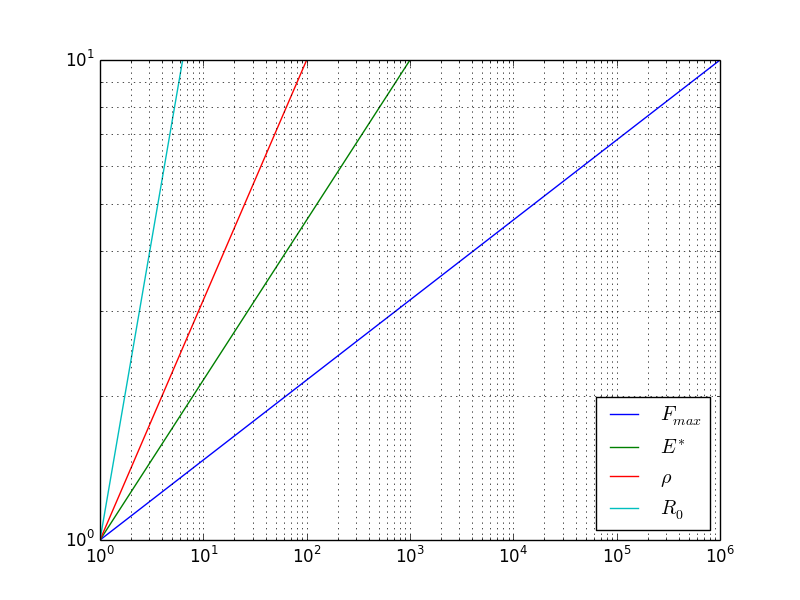
\includegraphics[width = 0.75 \textwidth]{chapters/figures/stability_curves}
% \caption{Curves showing the rate of response to timestep on the various normal-contact parameters.}\label{fig:stability-curves}
% \end{figure}

% It is apparent that simulations become less stable primarily as the pebble diameter decreases and then slightly less so for decreasing density and increasing the effective Young's modulus. It takes a rather large increase in the maximum contact force to cause the stable timestep to decrease. This is a fortunate result as it is primarily material properties which dictate stability of a DEM simulation. If external pressures increase and cause increases in the maximum normal contact force in the ensemble, it is unlikely to cause instabilities in the model. The result also provides insight into scaling of physical parameters to allow larger timesteps and thereby shorter overall duration of simulations.

The ceramic materials identified for breeders have relatively high Young's moduli, on the order of \si{10^{10} Pa}. The smallest radius will be on the order of \si{10^{-4} m}. The ceramic density is approximately on the scale of \si{10^{4} kg/m^3}. These values lead to a necessary timestep of

\begin{equation}
	\delta t_c \propto 10^{-7} \si{s}
\end{equation}

For a simulation that may last several hundreds of seconds of real time, this then requires more than 10$^9$ timesteps. If we have 10$^4$ particles in the simulation, each having their position integrated over a billion times, it becomes obvious that computational time is a major issue for our simulations of nuclear heating of ceramic breeder pebbles. If we are able to reduce the critical timestep (while perhaps decreasing the simulation time), the simulations will be much more practical for research use.
%~~~~~~~~~~~~~~~~~~~~~~~~~~~~~~~~~~~~~~~~~~~~~~~~~~~~~~~~~~~~~~~~~~~~~~~~~~~~~~~~




%~~~~~~~~~~~~~~~~~~~~~~~~~~~~~~~~~~~~~~~~~~~~~~~~~~~~~~~~~~~~~~~~~~~~~~~~~~~~~~~~
\subsection{Critical thermal timestep}

In \S\ref{sec:ht-pebble-conduction}, we introduced the dynamics of heat transfer between contacting particles in an ensemble. As we integrate the energy of an individual particle in time, we must also ensure that energy would not propagate through a particle faster than a single timestep can capture. In analogy to the critical timestep for mechanical stability (e.g. Eq.\ref{eq:rayleigh-stability-time}), we write for particle $i$,

\begin{equation}
	\delta t_\Bi = \frac{\rho_i C_i V_i}{H_c}
\end{equation}

where $\rho_i C_i V_i$ represents the inertial resistance to changing the temperature of $T_i$ and the conductance, $H_c$ represents the speed at which energy is delivered to $T_i$ from contact conduction. Then from the definition of $H_c$ we have given for smooth elastic spheres, this is also written as

\begin{equation}
	\delta t_\Bi = \frac{(4/3)\pi R_i^2\rho_i C_i}{2k^*}\frac{R_i}{a}
\end{equation}

For the material properties of lithium ceramics, as discussed for mechanical stability, we can expect

\begin{equation*}
	\frac{(4/3)\pi R_i^2\rho_i C_i}{2k^*} \approx \frac{(10^{-4})^210^{4}10^3}{10^0} = 10^{-1}
\end{equation*}

But from the requirements on Hertz theory in \S\ref{sec:hertz-contact}, we have required that $\frac{a}{R_i} \ll 1$. Thus the timestep for stability in the energy calculation is utterly negligible compared to the mechanical stability.

Vargas and McCarthy\cite{Vargas2001} make similar arguments, giving the criteria as,

\begin{equation}
	\frac{\mathrm{d}T_i}{T_i - T_j} \ll 1
\end{equation}

and too note that the timestep requirement for thermal calculations are orders of magnitude less restrictive than the analogous restriction of the particle dynamics.

Thus we can be confident that any timestep chosen for dynamic stability in the DEM simulation will automatically satisfy the timestep for thermal stability. 
%~~~~~~~~~~~~~~~~~~~~~~~~~~~~~~~~~~~~~~~~~~~~~~~~~~~~~~~~~~~~~~~~~~~~~~~~~~~~~~~~





%~~~~~~~~~~~~~~~~~~~~~~~~~~~~~~~~~~~~~~~~~~~~~~~~~~~~~~~~~~~~~~~~~~~~~~~~~~~~~~~~
\subsection{Simulation acceleration with scaled material properties}

We rewrite Eq.~\ref{eq:rayleigh-timestep} to facilitate a discussion on the parameters. Isolating each material term (neglecting the Poisson ratio) gives, 

\begin{equation}
	\delta t_c \propto R_i \times \rho_i^{1/2} \times E_i^{-1/2}
\end{equation}

% [pretty sure the approximation for $\nu$ only works when it's less than 1 so can't scale. must find out for sure.]

% The most direct effect would come from scaling the radius 





% From Makse\cite{Makse2004}

% We choose the time step to be a fraction of the time that it takes for a sound wave to propagate on the grain. Moreover, the quasistatic approximation used to calculate the Hertz force is valid only when the relative velocities of the par- ticles is smaller than the speed of sound in the grains\cite{Brilliantov1996}. Thus the characteristic time is $t_0 = R\sqrt{\rho_r/\mu_r}$ Typically, one chooses a time interval much smaller than the characteristic time, then $\Delta t=aR \sqrt{\rho_r/\mu_r}$ with $a<1$. Typical values for glass beads are:
% \si{\rho =2600 kg/m^3}, \si{\mu_r = 29 GPa}, \si{R = 0.1 mm}. Then $\Delta t$ should be smaller than \si{10^{−8} s}. Thus in order to perform a simulation over one second, more than $10^8$ steps are needed, which is obviously a very intensive computation. In this case, it is customary to increase the density or decrease the rigidity of the particles to allow for a larger time step to integrate the equations of motion over realistic periods of time. If the shear modulus of the grains in decreased, then it should be checked that the resulting stresses are several order of magnitude smaller than $\mu_r$, thus ensuring the condition of a nearly rigid system even though $\mu_r$ is taken smaller to obtain larger timesteps.

\section{Pebble failure modeling}
\label{failureDiscussion}
%In modeling pebble failure, there are two main tasks. The first is to develop a model for predicting a pebble failure event; { i.e.} what load (mechanical or thermal) will cause a pebble to crack, shatter, fracture, etc. The second is to develop a model which simulates the failure of that pebble; { i.e.} a scheme to treat a cracked, shattered, or crushed pebble in the assembly. 

The discrete element method has been used for studies in a variety of fields for studying inter-particle forces and the homogeneously distributed force networks that arise in packed beds (for example, see Ref.~\cite{Makse2000}). The discrete element method was also used in the fusion community to attempt to model failure initiation and propagation\cite{Annabattula2012a, Zhao2012, Zhao2013}. They too observed that a relatively few number of high-force networks, distributed troughought the bed supported the external mechanical loads. The even distribution of the force networks was used to defend the development of a probability-based predictor for failure. We make use of the probability argument of Zhao, {et al.} for the current study\cite{Zhao2013}. Their basic premise is that probability distributions of strength curves for pebble crushing have been observed (see, for example crush loads of Ref.~\cite{Tsuchiya1998}). Then in DEM models, a probability distribution of inter-particle forces are also observed. Overlaying the two probabilities resulted in seemingly random locations of pebbles satisfying the failure criteria -- not strictly along the high-force chains running through packed beds.

We apply the theory of Zhao, { et al.} in the following manner. If pebbles fail at random locations, we may de-couple the task of predicting pebble failure ({ i.e.} finding the mechanical or thermal load that causes a pebble to fail) from the task of modeling the ramifications of pebble failure. In our model, we begin with a starting point of a packed bed and then simply flag pebbles at random for `failing'. For our first model of failure, after a pebble has been flagged it is removed from the system entirely. The removal disrupts the meta-static state of the ensemble and the remaining pebbles re-settle. In reality, the ceramic pebbles generally break into just a few large pieces that remain in the system. Under development is a method for recreating that behavior in the DEM domain, it will be reported in future studies.

%Experiments on crushing single, brittle pebbles reveal that there are a number of failure modes\cite{Wu2004}. At one end, the pebble may simply crack and continue to hold a load for some time. At the other extreme, a pebble may crush virtually into a dust. We concern ourselves with the latter for this study. When a pebble in our simulation has been flagged for failure, we remove the pebble completely from the ensemble and then allow the remaining pebbles to rearrange to compensate for the lack of equilibrium on their contact forces. 


%\section{Simulation methods}
%\label{back} 
\section{DEM solver}\label{sec:dem-solver}

\subsection{Numerical Implementation Overview}

The primary computational tools used in this study is LAMMPS (Large-scale Atomic/Molecular Massively Parallel Simulator)\cite{Plimpton1995}; a classical molecular dynamics code. The package of code, maintained by Sandia National Labs (http://lammps.sandia.gov), has many features making it particularly attractive for our use on the simulation of pebble beds. LAMMPS is open-source and written in highly-portable C++ allowing customization of any feature used in modeling. LAMMPS runs with distributed-memory message-passing parallelism (MPI) and provides simple control (manual or automatic) of the spatial-decomposition of simulation domains for parallelizing. Perhaps most importantly, LAMMPS provides an efficient method for detecting and calculating pair-wise interaction forces; the largest consumer of run-time in the DEM algorithm\cite{Plimpton1995}. We build the code as a library so that LAMMPS can be coupled to other numerical tools; we use the scripting language of Python (Python 2.7) as an umbrella code to call LAMMPS routines with the full availability of Python libraries. 

LAMMPS by default provides a rudimentary method of modeling of granular particles (the term `granular' here differentiates the `discrete element' of molecules or atoms from larger-scale granular particles of powders or pebbles); LAMMPS has been used for studying granular material since at least 2001 when Silbert, et al.\cite{Silbert2001} studied granular flow on inclined planes. However, the usefulness of LAMMPS for studying granular systems was greatly enhanced by LIGGGHTS (LAMMPS Improved for General Granular and Granular Heat Transfer Simulations), a suite of modules included on top of LAMMPS. LIGGGHTS has many academic and industrial contributors from around the world, with the code maintained as open-source by DCS Computing, GmbH.

Briefly, some notable features the LIGGGHTS code brings to the LAMMPS environment include: Hertz/Hooke pair styles with shear history, mesh import for handling wall geometry, moving meshes, stress analysis of imported meshes, a macroscopic cohesion model, a heat transfer model, and improved dynamic load balancing of particles on processors\cite{Kloss2011}. Both LIGGGHTS and LAMMPS are distributed under the open-source codes under terms of the Gnu General Public License.

We will review some of the important physical models used in LAMMPS/LIGGGHTS as they relate to the important features we wish to investigate for packed beds of pebbles in fusion reactors.

\subsection{other solver info}

Time-discretization of the integration of Eq.~\ref{eq:newtons-second} is handled by the core Large-scale Atomic/Molecular Massively Parallel Simulator (LAMMPS) code released by Sandia National Laboratories\cite{Plimpton1995}. The code calculates velocity and position via the semi-explicit velocity-Verlet integration. The algorithm is stable with a global error of approximately $O(\Delta t^2)$ for displacement; details can be found in Ref.~\cite{Grubmuller1991}.

In the process of the study, to demonstrate the ability of the dynamic integration to capture resettling (and any possibly asymmetries), some beds were generated wherein the failure of pebbles was slightly localized near one or both $x$-walls. The profile of the pebbles near the top of the stack, after resettling, are shown in Fig.~\ref{fig:settlingStudy}. 

In our work, we occasionally required a fully quiesced bed. To determine when this occurred, the total kinetic energy of the entire ensemble was monitored and a packed bed was considered to have completely settled once the kinetic energy of the system was less than $10^{-9}$; similar to the process described in Ref.~\cite{Silbert2002}. 


The granular heat transfer equations are layered onto the LAMMPS code via a package of code named LIGGGHTS (LAMMPS Improved for General Granular and Granular Heat Transfer Simulations \cite{Kloss2012}). Parallelization of the code is straightforward with LAMMPS and we run the code on 128 nodes of UCLA's Hoffman2 cluster for typical run times of 18 to 24 hours per routine ({e.g.} filling, packing, heating, etc.).




%%%%%%%%%%%%%%%%%%%%%%%%%%%%%%%%%%%%%%%%%%%
\chapter{Modeling CFD-DEM} \label{modelingCFDEM}
%%%%%%%%%%%%%%%%%%%%%%%%%%%%%%%%%%%%%%%%%%
[talk about how lacking the DEM result is without the inclusion of helium in analysis. There are some Fusion papers on conductivity in vacuum and with helium]

We now consider the influence of helium on thermal transport of deposited nuclear energy as it is carried away by the cooled structural walls. We begin by considering the fluid in a continuum sense and the pebbles in a discrete one. The interactions of the fluid and solid are characterized by effective relationships in each discretized cell of fluid. We then consider an mesoscopic approach to the fluid-solid interaction with the Lattice-Boltzmann method. 

The chapter begins with introduction of the coupled fluid dynamics - discrete element method (CFD-DEM) approach: governing equations, discretization techniques, and algorithms.

We then do LBM. And stuff.

%%%%%%%%%%%%%%%%%%%%%%%%%%%%%%%%%%%%%%%%%%
\section{Numerical Methodology}
% From TOFE 2014
Models based on the discrete element method (DEM) are currently the only tools available that can extract information on individual pebble interactions. The DEM formulation provides information such as inter-particle forces and individual particle temperatures, which are necessary for predicting and simulating morphological changes in the bed (e.g. pebble cracking, sintering, etc.) However DEM alone is not able to capture the effects, neither on momentum nor energy, of an interstitial fluid. Therefore we present two fluid modeling techniques to supplement the DEM computations. We will first discuss the fully dynamic coupling of the DEM model with a volume-averaged thermofluid model of helium. Then we will introduce the integration of our DEM packing structure into lattice-Boltzmann simulations of the entire bed-fluid system.

\subsection{DEM}\label{sec:cfdem-heat-transfer}
The discrete element framework introduced in \S~\ref{sec:particle-dynamics} is augmented with a drag force term to capture interaction with surrounding fluid velocity fields. To accomplish this, we simply include a drag force to the Newtonian balance of forces given in Eq.~\ref{eq:newtons-first}. The momentum balance now reads:

\begin{equation}\label{eq:cfdem-dem-momentum}
	m_i  \ddt{\vec{r}_i} = m_i\vec{g} + \vec{f}_i + \beta_i V_i \Delta u_{if}
\end{equation}

where $\Delta u_{if} = u_f - u_i$, is the relative velocity between the fluid and pebble, $i$, and the inter-phase momentum exchange coefficient, $\beta_i$, acts upon the pebble volume (not to be confused with the damping coefficient introduced in \S~\ref{sec:particle-dynamics}). Similarly, the energy equation now includes 

\begin{equation}\label{eq:cfdem-dem}
	m_iC_i \ddt{T_i} = Q_{n,i} + \sum_{j=1}^Z Q_{ij} + \beta_{E,I} A_i \Delta T_{if}
\end{equation}

where $\Delta T_{if} = T_f - T_i$, is the relative temperature between teh fluid and pebble, $i$, and the inter-phase energy exchange coefficient, $\beta_{E,i}$, acts upon the pebble surface area, $A_i$.

The trajectory of pebble $i$ is updated based on the force terms on the right hand side of Eq.~\ref{eq:cfdem-dem}: gravity, contact forces between particles (or particle-wall), and a drag force. Similarly, the temperature of the particle updates with the terms from Eq.~\ref{eq:cfdem-dem-energy}: nuclear heating rate, inter-particle conduction, and now a heat transfer with surrounding fluid.

Drag forces from fluid flows through packed beds are found from volume-averaged, empirical correlations of either numerical or experimental studies. Considering a small region of a packed bed surrounding our particle of interest, i, the nondimensional drag force is found only as a function of the local packing fraction of that region. In the zero Reynolds number limit, the nondimensional drag force reduces to a Stokes flow correlation that is only a function of the local packing fraction value, $\phi$. For the value of particle Reynolds numbers seen by the helium purge gas, this is the dominant term. However, for a complete discussion of the nondimensional drag terms see Refs. 5, 6. The correlation used in this study comes from the results of numerical studies of packed beds by Koch and Hill~\cite{Koch2001, Gruber2012, Benyahia2006}. To arrive at their relationships, they did many lattice-Boltzmann simulations of porous flow.

\begin{equation}
	\beta_{i} = \frac{18\nu_f\rho_f}{d_{i}^2}(1-\phi) F
\end{equation}

where 

\begin{equation}
	F = \epsilon (F_0 + \frac{1}{2}F_3 \Re_{p,i})
\end{equation}

Stokes flow

\begin{align}
F_0 = 
	\begin{cases}
    		\frac{1+3\sqrt{\phi/2} + (135/64)\phi\ln(\phi) + 17.14\phi}{1 + 0.681\phi - 8.48\phi^2 + 8.16 \phi^3}	& \text{if } \phi < 0.4\\
    		10\frac{\phi}{(1-\phi)^3}              																& \phi > 0.4
	\end{cases}
\end{align}

and high Reynolds contribution

\begin{equation}
	F_3 = 0.0673 + 0.212\phi + \frac{0.0232}{(1-\phi)^5}
\end{equation}



The packing fraction and  void fraction in any fluid cell is calculated by summing through all the volumes of $k$ particles located in that cell (or the complement thereof)

\begin{equation}
	\phi = \sum_{i=1}^k \frac{V_{p,i}}{\Delta V_f}
\end{equation}

% \begin{equation}
% \epsilon = 1 - \sum_{i=1}^k \frac{V_{p,i}}{\Delta V_f}
% \end{equation}
Other forces, such as Magnus forces, are inconsequential on predominantly stationary packed beds and are not considered.



The inter-phase energy transfer coefficient is of the same form as a traditional heat transfer coefficient and is calculated from the Nusselt number for the helium flow (with conductivity $k_f$) through a packed bed.

\begin{equation}
	\beta_{E,i} = \frac{\Nu_i k_f}{d_i}
\end{equation}

Li and Mason\cite{Li2000} summarize correlations for Nusselt number as a function of Reynolds number for packed beds with the following equations
\[
\Nu= 
\begin{cases}
    2 + 0.6(1-\phi)^n\Re_p^{1/2}\Pr^{1/3}											& \Re_p < 200 \\
    2 + 0.5(1-\phi)^n\Re_p^{1/2}\Pr^{1/3} + 0.2(1-\phi)^n\Re_p^{4/5}\Pr^{1/3}   & 200 < \Re_p \le 1500 \\
    2 + 0.000045(1-\phi)^n\Re_p^{9/5}												& \Re_p > 1500
\end{cases}
\]
where $n=3.5$ was found to fit best for small particles in dilute flows. [we should find a new value for high packing fraction] 

Thus we have a formulation whereby a known fluid flow field and temperature throughout the domain, we can calculate the influence of that fluid on every particle’s position and temperature. Next we will cover how we can calculate the flow field based on a volume-averaged influence of particles on the fluid.




\subsection{Volume-averaged CFD Helium}
The technique of coupling CFD to DEM was first proposed by Tsuji, et al9. In this formulation of the helium flow, a fluid cell is much larger than the individual particles (in application, this meant approx. 5~6 particles per cell) and as such, the particles themselves are not resolved in the fluid space but are simply introduced via volume-averaged terms. Therefore momentum and energy of a fluid flow through a solid phase is governed by volume-averaged Navier-Stokes and energy equations10. These equations are applied to a discretized volume of fluid space. For fluid cell, k, these are5:



\begin{align}
\pder[\epsilon_k \rho_f]{t} + \nabla\cdot(\epsilon_k u_f \rho_f) &= 0\\
\pder[\epsilon_k u_f]{t} + \nabla\cdot(\epsilon_k u_f u_f) &= -\frac{\epsilon_k}{\rho_f}\nabla P_f + \nabla\cdot\left(\nu_f\epsilon_k\nabla u_f\right) - \frac{S_k}{\rho_f}\\
\pder[\epsilon_k T_f]{t} + \nabla\cdot(\epsilon_k u_f T_f) &= \nabla\left(\epsilon_k\epsilon\nabla T_f\right)-\frac{E_k}{\rho_fC_f}
\end{align}

where the fluid void fraction is the complement of the solid packing fraction, $\epsilon = 1 - \phi$. The momentum and energy exchanges with the solid phase are represented in the source terms. They are volume-weighted sums of the drag forces and energy exchanges, respectively, for all particles in the discretized fluid cell:

\begin{align}
S_k &= \frac{1}{V_k}\sum_{\forall i \in k} \beta_i V_i \Delta u_{if}\\
E_k &= \frac{1}{V_k}\sum_{\forall i \in k} \beta_{E,i} A_i \Delta T_{if}
\end{align}

The inter-phase momentum and energy exchange coefficients act as the communicators between the particle information from the DEM solver and the fluid fields from CFD. Thus the motion and energy of the fluid field are intimately coupled with the particle positions and energy, but computational time is preserved by only considering volume-averaged values in the fluid domain. The cross-communication between fluid and solid is accomplished with a coupling routine that is explained in detail in Refs. 11, 12.


% In the discrete element method, we showed the forces acting on a particle with Eq.~\ref{NewtonsFirst}. It is given again here,
% \begin{align*}
%  F_i = m_i g + \sum_{j}^Z&\left(k_n\delta_{n_{ij}} - \gamma_n v_{n_{ij}}\right) + \left(k_t\delta_{t_{ij}} - \gamma_t v_{t_{ij}}\right)
% \end{align*}

% The influence of the fluid phase is introduced through a new drag force term, $f_{d,i}$:
% \begin{align}
%  F_i = m_i g + f_{d,i} + \sum_{j}^Z&\left(k_n\delta_{n_{ij}} - \gamma_n v_{n_{ij}}\right) \left(k_t\delta_{t_{ij}} - \gamma_t v_{t_{ij}}\right)
% \end{align}




\subsection{Modeling Setup and Procedure}
The pebble bed has dimensions in the x-y directions of 20d×15d, respectively. There are structural walls, providing cooling, at the x-limits and periodic walls in the y-limits. 10 000 pebbles were loaded into the system which went to a height of approximately 24d after the bed was vibration packed. The pebble bed had a roof loaded at the upper limit of the z-direction that was lowered by force-control up to 6 MPa. This bed is referred to as the ‘well-packed’ bed. This was meant to simulate a fresh, densely-packed bed that is under compressive load during fusion operation. As such, this would be when pebbles would be likely to crack during operation. Therefore, based on the well-packed bed, a second bed was generated by simulating crushed pebbles; crudely the extensive crushing is simulated by simply removing 10\% of the pebbles at random from the ensemble and then allowing the bed to resettle, from the now-imbalanced gravity and inter-particle forces, to a new stable packing structure. This bed is then referred to as the ‘resettled’ bed for the rest of the analysis. The intent is to deduce changes in thermomechanical properties from an ideally packed bed to one where significant cracking has altered the ideal morphology of the bed.
\subsection{Pressure Drop}
Before analyzing thermal results from the CFD-DEM coupling, the system was run at various particle Reynolds numbers and the overall pressure drop of the packed bed was measured. This value was compared against the well-known Kozeny-Carman and Ergun equations. The Kozeny-Carman is known to fit better with experimental data at very small Reynolds numbers. In Fig. 1 we see the CFD-DEM coupling model is providing bed-scale pressure drops that match very well with Kozeny-Carman over the Reynold’s numbers applicable to helium purge flow in fusion reactors.
The flow is visualized in Fig. 2. The pebble bed is clipped at the centerline to allow viewing of the helium streamlines. Apparent in the figure is temperature profiles in the helium from centerline to wall that qualitatively mirror temperature profiles in the pebble bed.

\begin{figure}
        \centering
        \begin{subfigure}[b]{0.75\textwidth}
                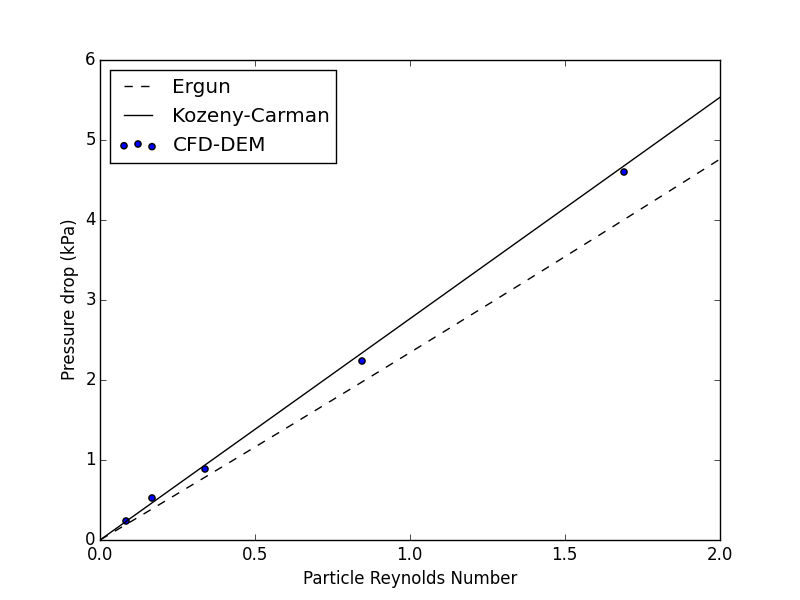
\includegraphics[width=\textwidth]{chapters/figures/pressureDrops-full.png}
                \caption{Well-packed bed}
                \label{fig:pressure-drop-full}
        \end{subfigure}%
        
          %add desired spacing between images, e. g. ~, \quad, \qquad, \hfill etc.
          %(or a blank line to force the subfigure onto a new line)
        \begin{subfigure}[b]{0.75\textwidth}
                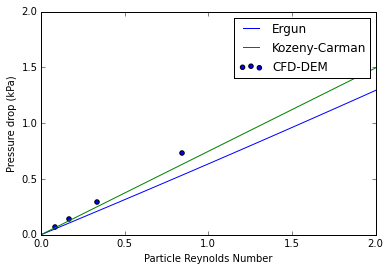
\includegraphics[width=\textwidth]{chapters/figures/pressureDrops-evap.png}
                \caption{Re-settled bed}
                \label{fig:pressure-drop-evap}
        \end{subfigure}
        \caption{Pressure drop calculations across packed beds, solved by CFD-DEM, fit well to the Kozeny-Carman empirical relation.}\label{fig:cfdem-pressure-drop}
\end{figure}



\begin{figure}[t]
	\centering
	\caption{Cut-away view of the pebble bed with streamlines of helium moving in generally straight paths from inlet to exit.}
	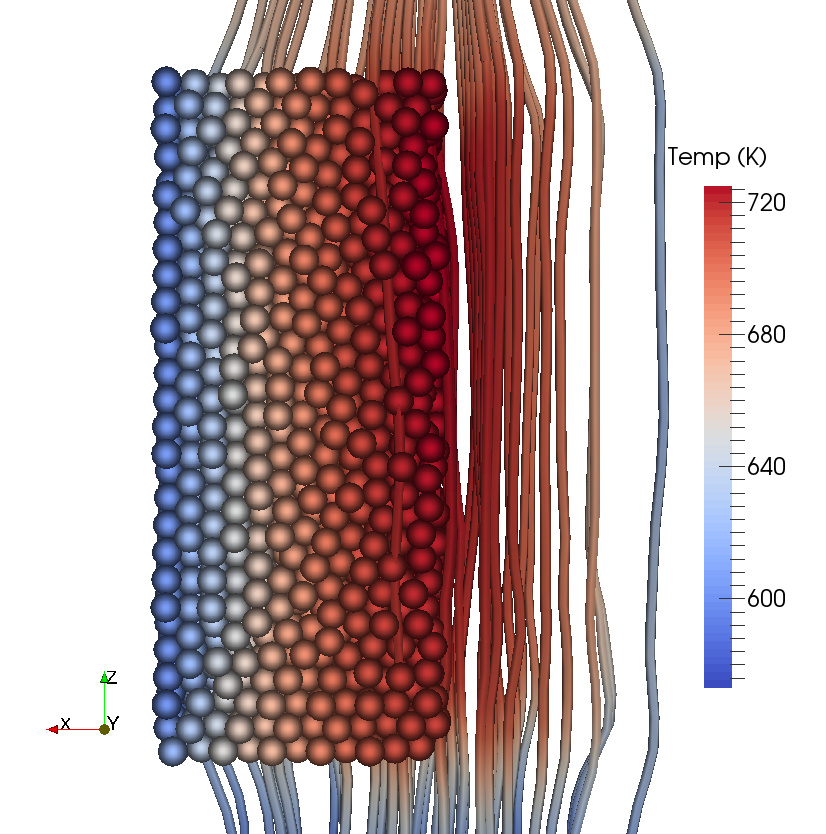
\includegraphics[width=0.75\textwidth]{chapters/figures/cfd-dem-streamlines2}\label{fig:cfdem-streamlines}
\end{figure}




\begin{figure}
        \centering
        \begin{subfigure}[b]{0.75\textwidth}
                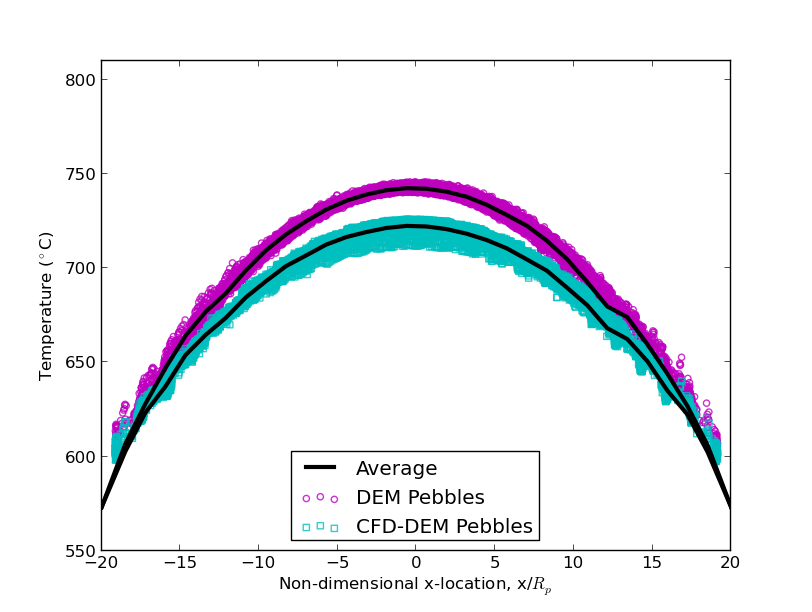
\includegraphics[width=\textwidth]{chapters/figures/full-x-T-color}
                \caption{Well-packed bed}
                \label{fig:x-T-full}
        \end{subfigure}%
        
          %add desired spacing between images, e. g. ~, \quad, \qquad, \hfill etc.
          %(or a blank line to force the subfigure onto a new line)
        \begin{subfigure}[b]{0.75\textwidth}
                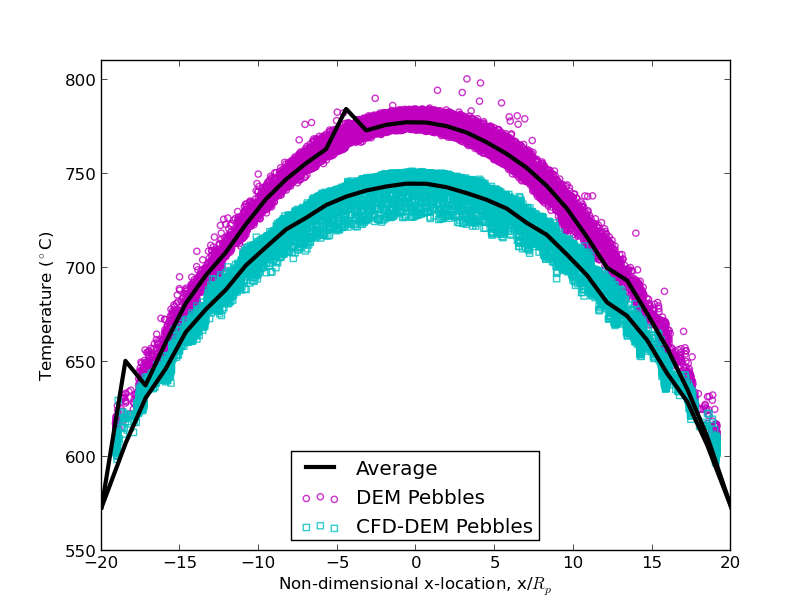
\includegraphics[width=\textwidth]{chapters/figures/evap-x-T-color}
                \caption{Re-settled bed}
                \label{fig:x-T-evap}
        \end{subfigure}
        \caption{Scatter temperature profiles of pebbles in a bed that is: well-packed (left) and resettled after 10\% of pebbles were removed from crushing (right). The introduction of helium into the simulation contributes to both lower overall temperatures (higher effective conductivity) and the smoothing out of high temperatures of isolated pebbles.}\label{fig:cfdem-x-T}
\end{figure}

\subsection{Effective thermal conductivity from CFD-DEM}

The well-packed and resettled pebble beds were run to thermal steady-state with nuclear heating and wall cooling in both pure DEM and coupled CFD-DEM simulations for comparison. From steady-state temperature distributions, seen in the pebble scatter plots in Fig. 3, an average profile is calculated and an effective thermal conductivity computed. The values are tabulated in Table I. 
In the case of pure DEM, energy is transported solely along conduction routes in the ensemble. When the packing of the bed is disturbed, this results in a substantial drop in effective conductivity (a drop of 31\%). The details of the conductivity reduction were studied extensively in Ref. 23. Perhaps more important than the reduction in effective conductivity, is the appearance of isolated pebbles. Because heat deposition is volumetrically applied, pebbles with poor conduction routes become much hotter than their neighbors. This is evident in the high temperatures seen in many of the pebbles in the right figure of Fig. 3. Over-heating of isolated pebbles could induce sintering and impact their tritium release even when the average temperatures measured in the bed are well below sintering values.
When CFD-DEM beds are analyzed, there is still a large reduction in effective conductivity (22\% drop), but interesting to note is the lack of isolated pebbles with high temperatures. In the CFD-DEM scatter plot of the right image in Fig. 3, there is evidence of the reduced heat transfer in the same region as the isolated pebbles from the DEM bed, but the temperatures are much closer to the average values of neighboring pebbles. The helium purge gas has effectively smoothed out the temperatures and provided heat transport paths for any pebbles that have loose physical contact with neighbors.
In spite of the 22\% decrease in effective conductivity, the maximum temperature of the pebble bed only increased 6.2\% (from 725 to 751 K) when helium is included in the model. This result is significant for solid breeder designers. They may choose a solid breeder volume such that in the event of extensive pebble cracking, the maximum temperature of the bed would remain within the ideal windows dictate for the lithium ceramics.

\begin {table}[htp] %
\caption{Pebble bed values from the test matrix of the beds analyzed in this study.}
\label {tab:cfdem-keff} \centering %
\begin {tabular}{ rccccc }
\toprule %
			& 	\multicolumn{2}{c}{$k_\text{eff}$}	&   \multicolumn{2}{c}{$T_\text{max}$}	&	$\frac{Q_h}{Q_\text{nuc}}$		\\
			& 	\multicolumn{2}{c}{(W/mK)}			&	\multicolumn{2}{c}{(K)}				&									\\
			& 	DEM 		& 	CFD-DEM				&	DEM 		& 	CFD-DEM 			& 	CFD-DEM							\\\toprule
Well-packed	& 	0.96		& 	1.09				& 	745			& 	725					& 	1.15							\\
Resettled	& 	0.66		& 	0.85				& 	800			& 	751					& 	1.52							\\\bottomrule
\end{tabular}
\end{table}




An accompanying result is the increased amount of energy carried out of the system by the helium purge gas. In Table I, the last column provides the ratio of energy carried out of the system to the nuclear energy deposited into the bed. The amount of energy carried out by the helium increased from 1.15\% to 1.52\% from ‘well-packed’ to ‘resettled’.
evap-x-T-color
The CFD-DEM formulation maintains calculations of pebble-pebble interactions while dynamically coupling to the helium flow. The model demonstrates the ability of helium gas to smooth out any hot spots predicted by pure-conduction DEM formulations. Further, the lattice-Boltzmann simulation, while not fully coupled to DEM, revealed important features of helium flow in volumetrically heated pebble beds – mainly the smearing of temperature profiles along the paths of cooling.
%%%%%%%%%%%%%%%%%%%%%%%%%%%%%%%%%%%%%%%%%%
%\chapter{Modeling lattice-Boltzmann Method (LBM)}\label{sec:modeling-lbm}
%%%%%%%%%%%%%%%%%%%%%%%%%%%%%%%%%%%%
\chapter{Pebble Interaction Analysis: Experimental Relationships} \label{sec:analysis-experiment}
%%%%%%%%%%%%%%%%%%%%%%%%%%%%%%%%%%%

Many experiments were carried out on individual ceramic pebbles. While there are some measures from experiments that are immediately useful for qualitative comparisons, such as the crush strength between different batches of ceramics, most values are not obviously connected to analysis of the pebbles nor the pebble bed assemblies they make up. In this section we will show had careful examination of single pebble experiments can lead to predictions of not only strength in ensembles but also modifications of the fundamental properties of the ceramic pebbles.

In section \S~\ref{sec:exp-reduction-factor}, we use single pebble experiments to validate the use of Hertz theory for contacting ceramic pebbles, but also determine the proper Young's modulus to use for the ceramics. In section \S~\ref{sec:exp-strain-energy} we use the theory we developed in section \S~\ref{sec:theory-strain-energy} along with experimental data to begin to make predictions for survivability of pebbles in ensembles.


\subsection{Elasticity Reduction Factor}\label{sec:exp-reduction-factor}

% the following was from the MOTIVATION section of SOFT-2014~~~~~~~~~~~~~~~~~~~~~~
% In the study of individual pebble crush force, the force-travel response curves of ceramic materials consistently exhibit distributions in the stiffness of the pebbles. For example, see the results of different lithium ceramic pebbles in Fig.~\ref{fig:force-travel-exp}. For DEM studies, we claim that interaction between these pebbles is well-represented by the Hertzian normal force as derived in \cref{sec:hertz-theory}. For the discussion, we rewrite Eq.~\ref{eq:hertz-normal-force} here,


% \begin{equation*}
%   F_{n,ij} = \frac{4}{3}E_{ij}^* \sqrt{R_{ij}^*} \, \delta_{n,ij}^{3/2}
% \end{equation*}

% where $\delta$ is the overlap between contacting spheres and $\frac{1}{E^*} = \frac{1-\nu_i^2}{E_i} + \frac{1-\nu_j^2}{E_j}$, $\frac{1}{R^*} = \frac{1}{R_i} + \frac{1}{R_j}$

% From Eq.~\ref{eq:hertz-normal-force}, we see the contact force is directly proportional to the pair Young's modulus, $E^*$. Thus an accurate value of pebble Young's modulus is critical for an accurate calculation of contact force. We now present Hertz equation as it applies to a pebble, diameter of $d_p$, being pressed between two flat anvils with measured travel of one anvil as $s$:

% \begin{equation}\label{eq:peb-anvil-contact-force}
%   F_n = \frac{1}{3}E^*\sqrt{d_ps^3}
% \end{equation} 

% and $\frac{1}{E^*} = \frac{1-\nu_p^2}{E_p} + \frac{1-\nu_a^2}{E_a}$. Where the subscript $p$ refers to pebbles and $a$ the anvils.

% From Eq.~\ref{eq:peb-anvil-contact-force}, we see that standard Hertz theory, where we use a single value for Young's modulus from literature, is not appropriate for pebbles studied in ceramic breeders. If single values of $E_p$ and $\nu_p$ are employed, then variation in pebble diameters can not alone explain the variation of curves of Fig.~\ref{fig:force-travel-exp}.
% %~~~~~~~~~~~~~~~~~~~~~~~~~~~~~~~~~~~~~~~~~~~~~~~~~~~~~~~~~~~~~~~



% \subsubsection{Elasticity reduction factor}
% We propose to explain the behavior of individual pebbles (as in Fig.~\ref{fig:force-travel-exp}) with an assumption that the production technique yields pebbles with slightly different internal structures. The differences in internal structure then cause the pebble to have a different apparent modulus of elasticity; which will vary from some strong limit value. The strong value is the elastic modulus of highly sintered pellets reported in literature for the material, $E_\text{bulk}$. Assuming this strong value is the upper limit, imperfections in the pebbles will lead only to a reduction in this value. To quantify the deviation from the bulk, we introduce a $k$ factor, defined as the elasticity reduction factor:

% \begin{equation}
%   k = \frac{E_\text{peb}}{E_\text{bulk}}
% \end{equation}
% where $k \in [0,1]$.

% If each pebble has a unique $k$ value, this would quantify the spread in elastic responses seen in the experiments. The value is found by assuming that the pebbles are, in fact, behaving in a Hertzian manner, allowing us to back-out its $k$ value, or in other words the unique $E^*$ of that pebble by finding a best fit to the experimental curves. 

% From room temperature, we take the sintered pebble value for these Li$_4$SiO$_4$ pebbles to be $E_\text{bulk} = 90$~GPa and $E_\text{bulk} = 124$~GPa for Li$_4$SiO$_4$ pebbles. Then we iterate over all values of $k\in[0,1]$ and compare the Hertzian response to that pebble's force-displacement curve.

% The data of Fig.~\ref{fig:nfri-force-travel-exp} is fit in the manner described and the pebbles are all plotted against Hertzian curves with their own unique modified Young's modulus in Fig.~\ref{fig:hertz-exp}. The modified Hertzian curves with apparent Young's modulus fits well with most of the pebbles' curves. Similar data is obtained for the pebbles of Fig.~\ref{fig:fzk-force-travel-exp} but the results are omitted for conciseness.


% \begin{figure}
%        \centering
%        \begin{subfigure}[b]{0.45\textwidth}
%                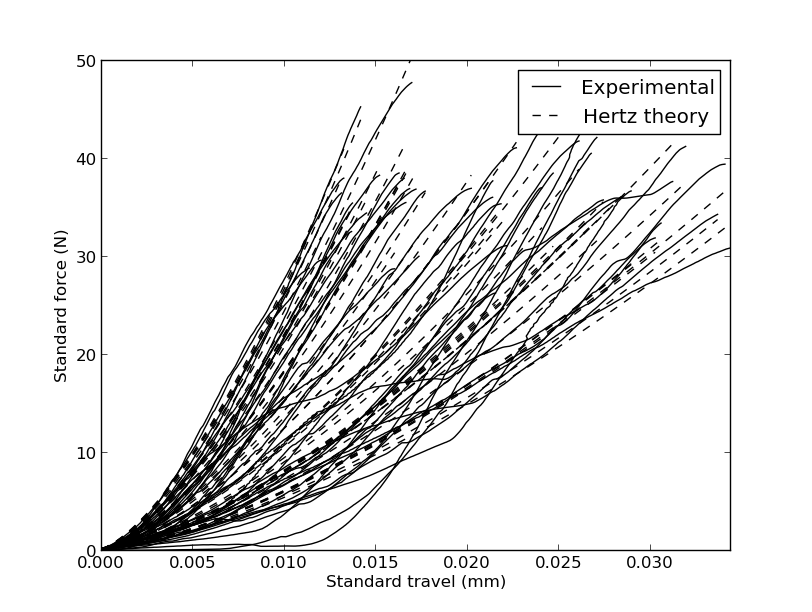
\includegraphics[width=\textwidth]{chapters/figures/NFRI-exp_v_hertz}
%                \caption{Experimental responses (solid) and fit curves of Hertzian equivalent with apparent Young's modulus (dashed).}
%                \label{fig:hertz-exp}
%        \end{subfigure}%
       
%         %add desired spacing between images, e. g. ~, \quad, \qquad, \hfill etc.
%          %(or a blank line to force the subfigure onto a new line)
%        \begin{subfigure}[b]{0.45\textwidth}
%                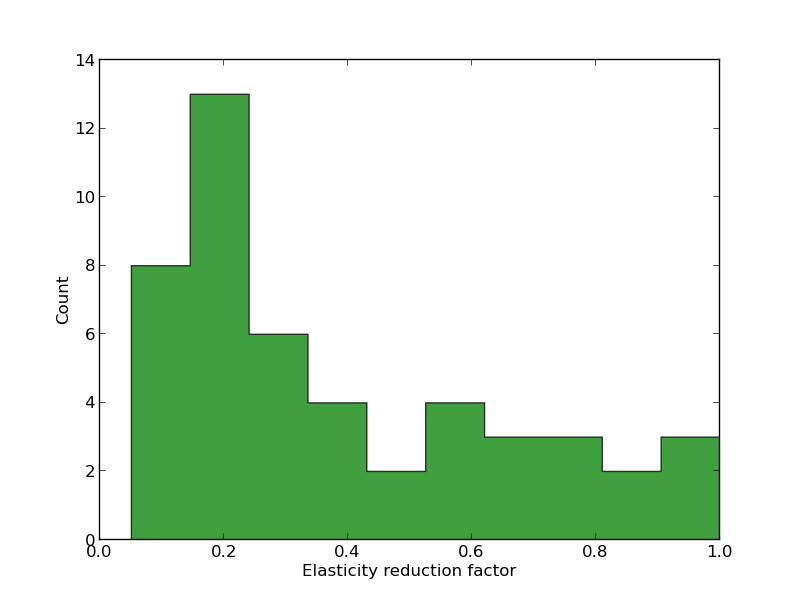
\includegraphics[width=\textwidth]{chapters/figures/NFRI-k_hist}
%                \caption{Distribution of elasticity reduction value, $k$, for the pebbles in this batch of lithium metatitanate. This distribution is modeled as a Weibull distribution function in DEM simulations.}
%                \label{fig:k-hist}
%        \end{subfigure}
%        \caption{An apparent Young's modulus is found for each pebble and the distribution of reduction factor, $k$, shows the quantity of reduction of the stiffness of the pebbles from the value found in literature.}
% \label{fig:hertz-results}
% \end{figure}




% \begin{figure}[t]
% \centering
% 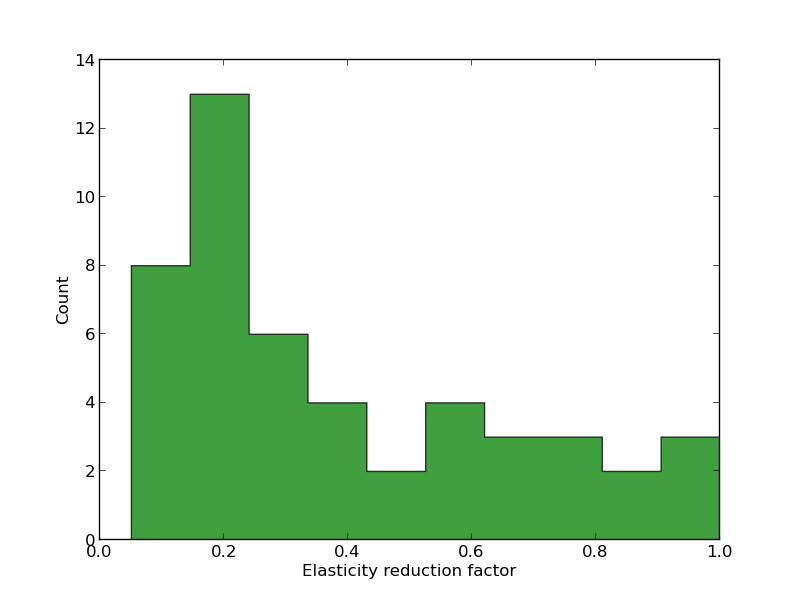
\includegraphics[width = 0.45 \textwidth]{chapters/figures/NFRI-k_hist}
% \caption{Distribution of elasticity reduction value, $k$, for the pebbles in this batch of lithium metatitanate. This distribution is modeled as a Weibull distribution function in DEM simulations.}\label{fig:k-hist}
% \end{figure}

% From the distribution of $k$, we see that the Young's modulus of many of the pebbles is about 20\% of the value of the sintered pellet that is given as the material property from literature. The Hertz contact force for these soft pebbles is then likewise 20\% of the value one would predict if using the Young's modulus from literature! 
% One of the benefits of using DEM simulations is the ability to predict pebble cracking in an ensemble based on knowledge of the interaction forces. If we are over-predicting the contact forces based on inaccurate material properties, we are going to be over-predicting the impact of pebble cracking as well. An accurate description of the material properties is an important feature for ceramic breeder designers.

% We will apply the modified Young's modulus distributions to pebble beds and compare the results to pebble beds simulated with standard Young's modulus from literature.

% \begin{figure}[t]
%   \centering
%   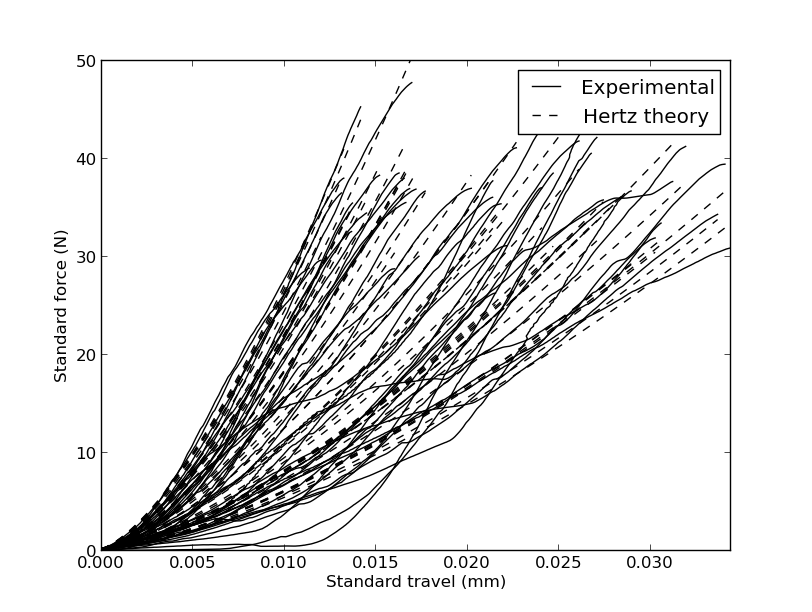
\includegraphics[width = \singleimagewidth]{chapters/figures/NFRI-exp_v_hertz}
%   \caption{Experimental responses (solid) and fit curves of Hertzian equivalent with apparent Young's modulus (dashed).}\label{fig:hertz-exp}
% \end{figure}

%end of the section taken from SOFT 2014 ~~~~~~~~~~~~~~~~~~~~~~~~~~~~~~~~





We introduced Hertz theory in \cref{sec:hertz-theory}, and in \cref{sec:modeling-dem} showed how we apply the Hertzian contact rules into the discrete element computational framework. We will revisit the Hertzian equations as we analyze the force-displacement measurements of single pebbles in the anvils of our uniaxial compression test stand.

The derivation to the Hertz force can be found on page~\pageref{eq:hertz-normal-force} but the result is given again here for reference:
\begin{equation*}
  F_{n,ij} = \frac{4}{3}E_{ij}^* \sqrt{R_{ij}^*} \, \delta_{n,ij}^{3/2}
\end{equation*}
and, again, the pair Young's modulus and radius are
\begin{align*}
\frac{1}{E^*} & = \frac{1-\nu_i^2}{E_i} + \frac{1-\nu_j^2}{E_j} \\
\frac{1}{R^*} & = \frac{1}{R_i} + \frac{1}{R_j}
\end{align*}

In experiments where we press a ceramic pebble between two platens, we measure the travel, $s$, rather than the pebble overlap, so we modify Eq.~\ref{eq:hertz-normal-force} to be represented in terms of travel ($s = 2\delta$). Furthermore, for a pebble ($R_i = R_p$) in contact with a smooth plane ($R_j \rightarrow \infty$), the relative radius is simply $R^* = R_p = d_p/2$. We write the Young's modulus of the pebble as $E_p$ and for the test stand's anvil as $E_s$; similarly for the Poisson ratios of the two materials. The Hertz force for a pebble between anvils is then

\begin{equation}\label{eq:contact-force}
        F = \left[\frac{1}{3}\frac{\sqrt{d_p}}{\frac{1-\nu_p^2}{E_p} + \frac{1-\nu_s^2}{E_s}}\right] s^{3/2}
\end{equation}


\begin{figure}[!t]
\centering
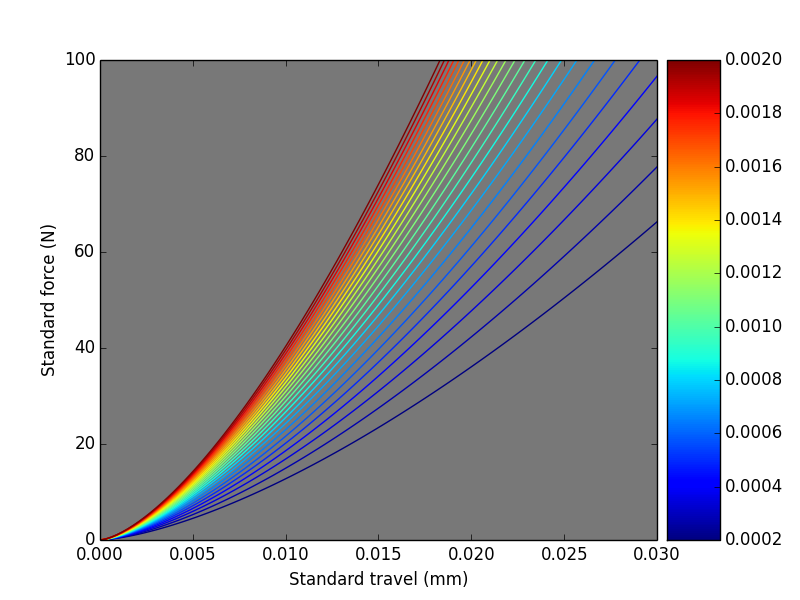
\includegraphics[width = \singleimagewidth]{chapters/figures/hertz-dp-dependence}
\caption{Hertzian responses of \lit pebbles compressed between platens. The colormap shows pebble diameters in \si{m}. The diameters span an order of magnitude from $d_p = \si{0.2 mm}$ to $d_p = \si{2 mm}$.}\label{fig:hertz-dp-dependence}
\end{figure}

\begin{figure}[!t]
\centering
    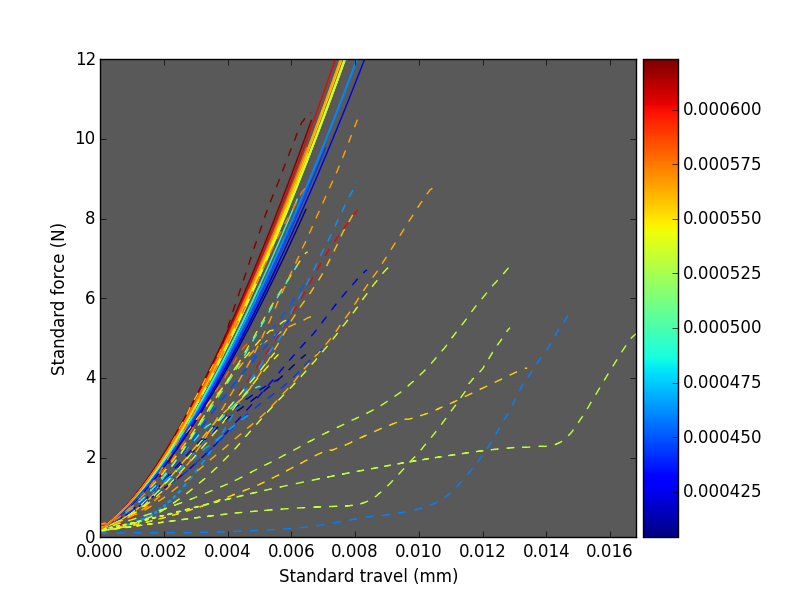
\includegraphics[width=\doubleimagewidth]{chapters/figures/fzk-data-w-ideal-hertz.png}
    \caption{Dashed lines are \lis pebbles of approximately \si{0.5 mm} diameter. Solid lines are the Hertzian (Eq.\ref{eq:contact-force}) responses based on each pebble's measured diameter.}
    \label{fig:fzk-exp-colormap}
\end{figure}

\begin{figure}
        \centering
        \begin{subfigure}[b]{\doubleimagewidth}
                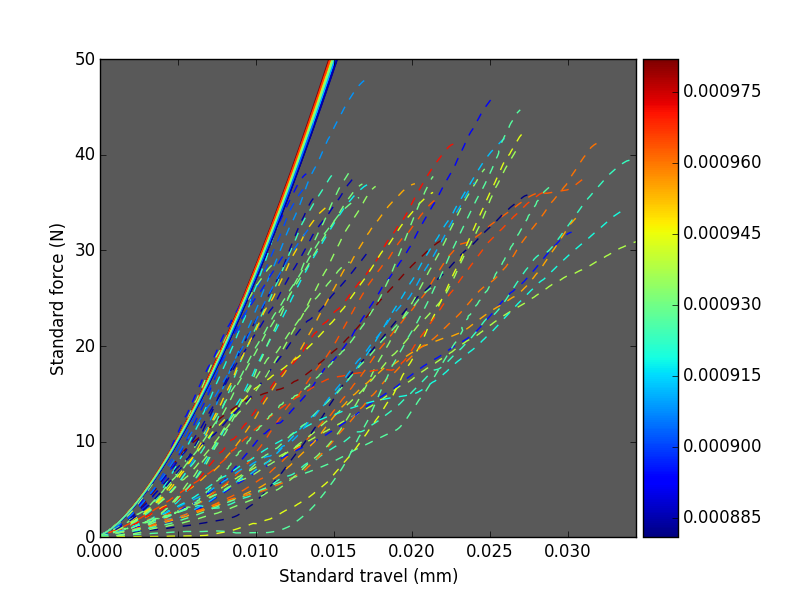
\includegraphics[width=\textwidth]{chapters/figures/nfri-1mm-data-w-ideal-hertz.png}
                \caption{$\bar{d}_p = 1$ mm}
                \label{fig:nfri-1-exp-colormap}
        \end{subfigure}
        ~
        \begin{subfigure}[b]{\doubleimagewidth}
                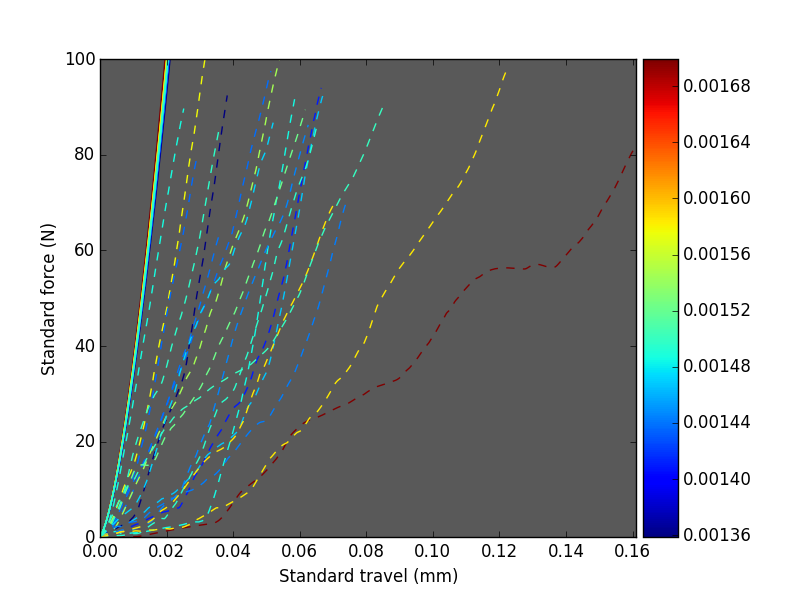
\includegraphics[width=\textwidth]{chapters/figures/nfri-1.5mm-data-w-ideal-hertz.png}
                \caption{$\bar{d}_p = 1.5$ mm}
                \label{fig:nfri-1.5-exp-colormap}
        \end{subfigure}
        \caption{Dashed lines are \lit pebbles. Solid lines are the Hertzian (Eq.\ref{eq:contact-force}) responses based on each pebble's measured diameter.}\label{fig:nfri-exp-curves}
\end{figure}


\begin{figure}[!t]
\centering
    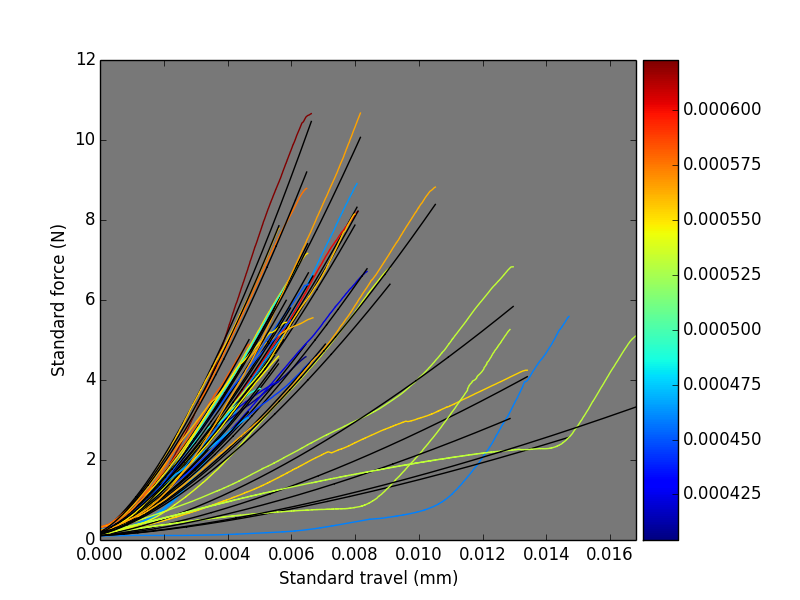
\includegraphics[width=\doubleimagewidth]{chapters/figures/fzk-hertz-colormap.png}
    \caption{Force-displacement curves for \lis pebbles (in color) along with their Hertzian fits (in black) calculated with each pebble having a unique Young's modulus.}
    \label{fig:fzk-exp-hertz}
\end{figure}

\begin{figure}
        \centering
        \begin{subfigure}[b]{\doubleimagewidth}
                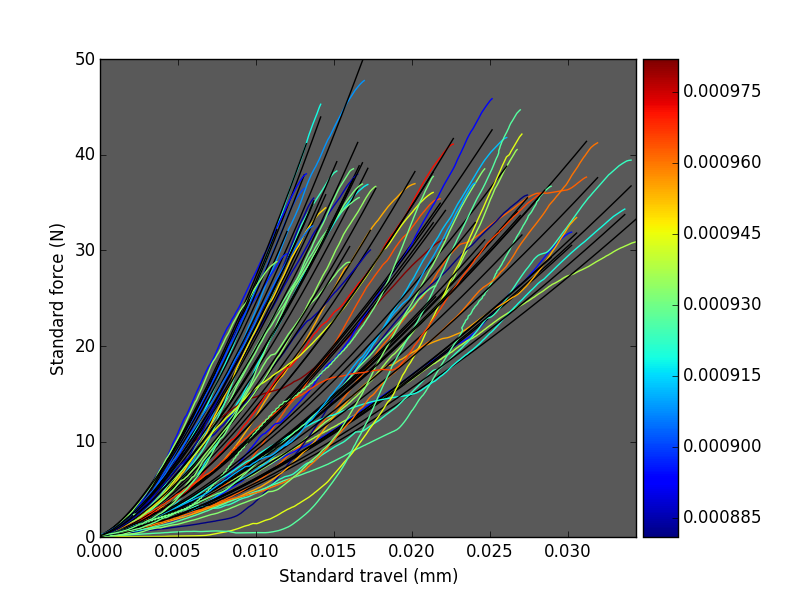
\includegraphics[width=\textwidth]{chapters/figures/nfri-1mm-hertz-colormap.png}
                \caption{$\bar{d}_p = 1$ mm}
                \label{fig:nfri-1-exp-hertz}
        \end{subfigure}
        ~
        \begin{subfigure}[b]{\doubleimagewidth}
                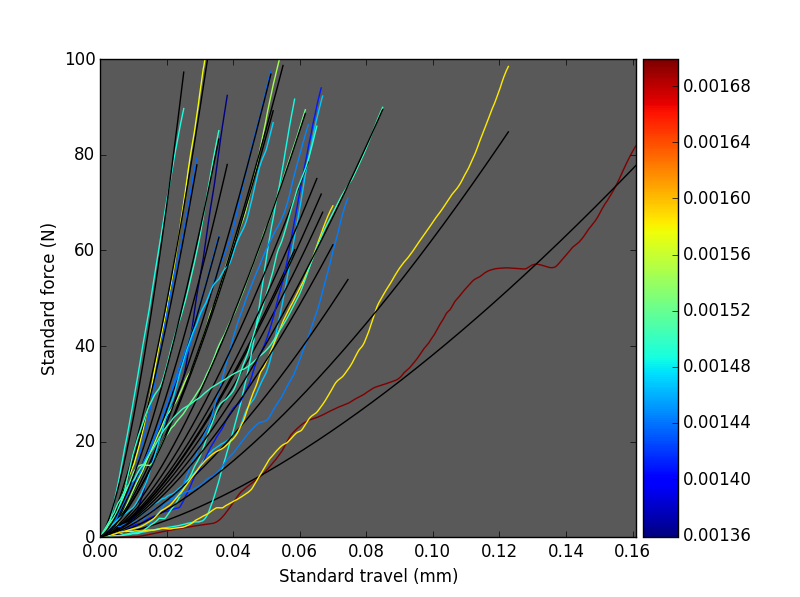
\includegraphics[width=\textwidth]{chapters/figures/nfri-1.5mm-hertz-colormap.png}
                \caption{$\bar{d}_p = 1.5$ mm}
                \label{fig:nfri-1.5-exp-hertz}
        \end{subfigure}
        \caption{Force-displacement curves for \lit pebbles (in color) along with their Hertzian fits (in black) calculated with each pebble having a unique Young's modulus.}\label{fig:nfri-exp-hertz}
\end{figure}

\begin{figure}[!t]
\centering
    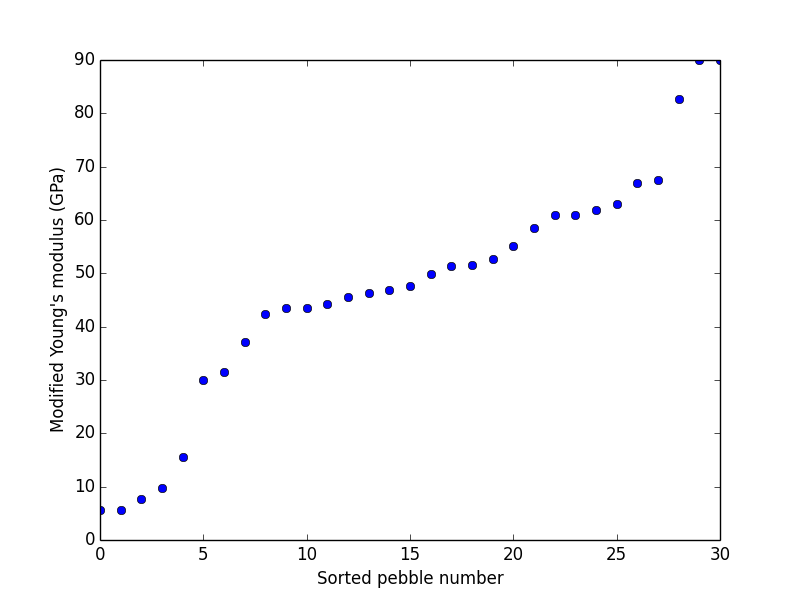
\includegraphics[width=\doubleimagewidth]{chapters/figures/fzk-E-plot.png}
    \caption{Distribution of modified Young's modulus for a batch of \lis pebbles. Most pebbles responded to compression with a Young's modulus well below the sintered pellet value of \si{90 GPa}.}
    \label{fig:fzk-E-plot}
\end{figure}

\begin{figure}
        \centering
        \begin{subfigure}[b]{\doubleimagewidth}
                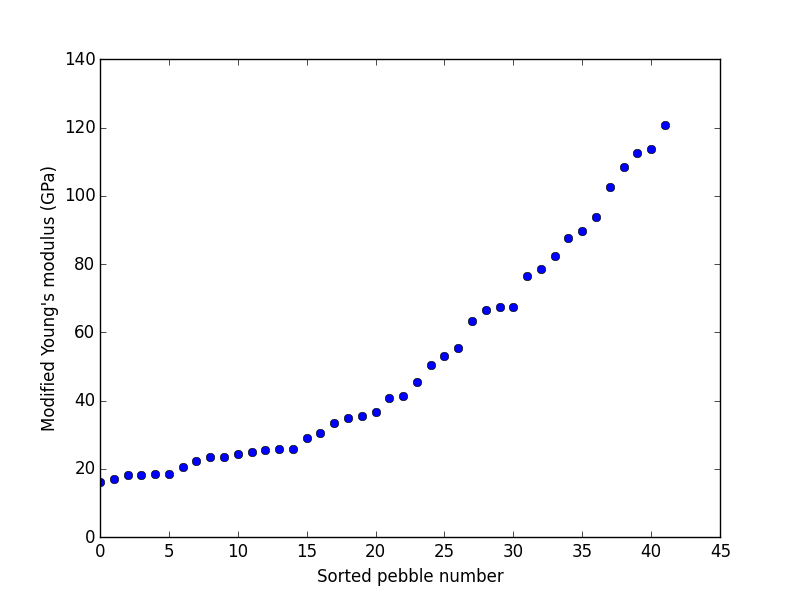
\includegraphics[width=\textwidth]{chapters/figures/nfri-1mm-E-plot.png}
                \caption{$\bar{d}_p = 1$ mm}
                \label{fig:nfri-1mm-E-plot}
        \end{subfigure}
        ~
        \begin{subfigure}[b]{\doubleimagewidth}
                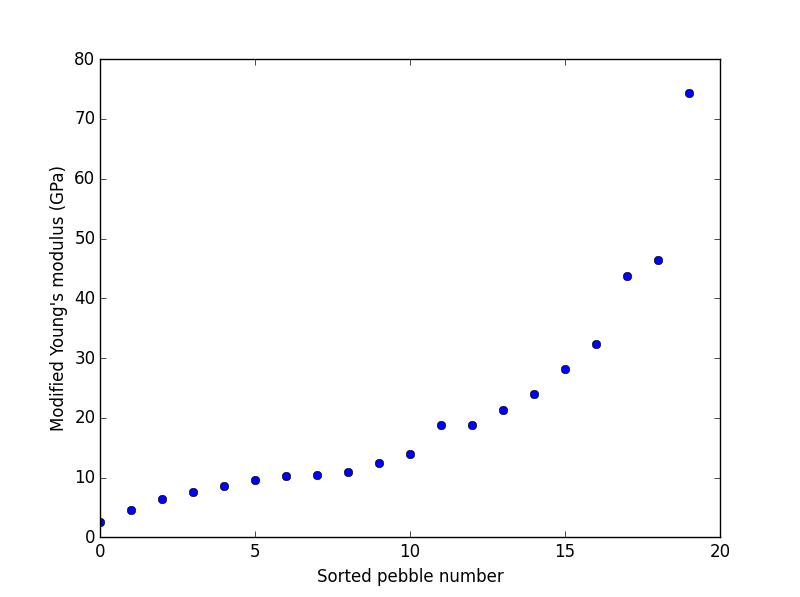
\includegraphics[width=\textwidth]{chapters/figures/nfri-1.5mm-E-plot.png}
                \caption{$\bar{d}_p = 1.5$ mm}
                \label{fig:nfri-1.5mm-E-plot}
        \end{subfigure}
        \caption{Distribution of modified Young's modulus for a batch of \lit pebbles. All pebbles responded to compression with a Young's modulus well below the sintered pellet value of \si{126 GPa}.}\label{fig:nfri-E-plot}
\end{figure}


\begin{figure}[!t]
\centering
    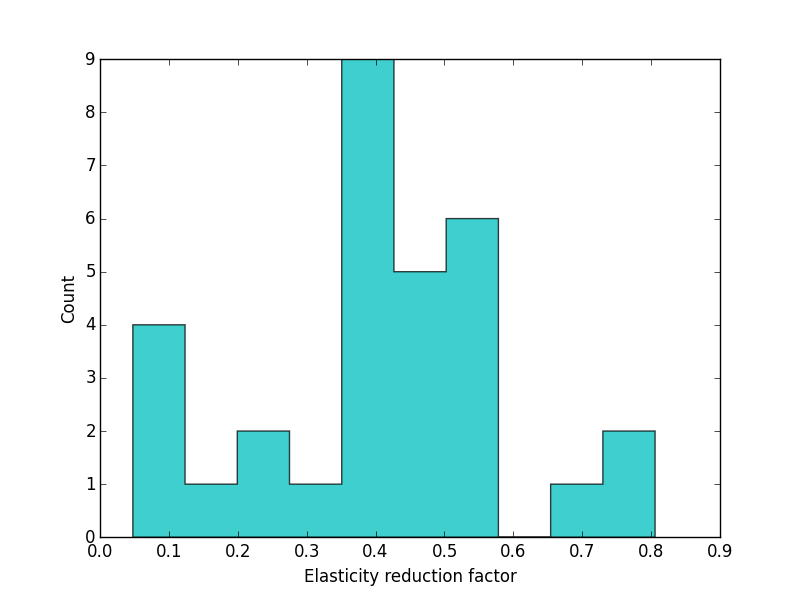
\includegraphics[width=\doubleimagewidth]{chapters/figures/fzk-kappa-histogram.png}
    \caption{Histogram of $\kappa$ for a batch of \lis pebbles. Most pebbles responded to compression with a Young's modulus well below the sintered pellet value of \si{90 GPa}.}
    \label{fig:fzk-kappa-hist}
\end{figure}

\begin{figure}
        \centering
        \begin{subfigure}[b]{\doubleimagewidth}
                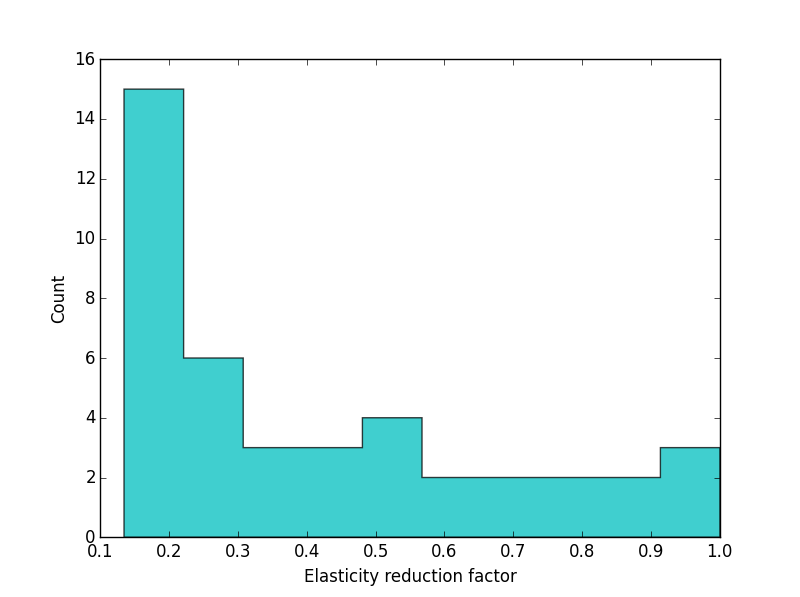
\includegraphics[width=\textwidth]{chapters/figures/nfri-1mm-kappa-histogram.png}
                \caption{$\bar{d}_p = 1$ mm}
                \label{fig:nfri-1mm-kappa-hist}
        \end{subfigure}
        ~
        \begin{subfigure}[b]{\doubleimagewidth}
                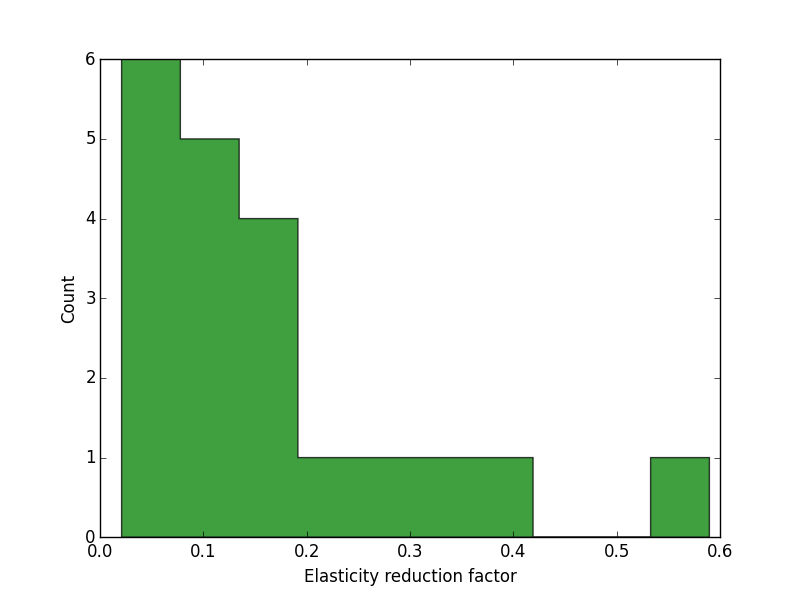
\includegraphics[width=\textwidth]{chapters/figures/nfri-1.5mm-kappa-histogram.png}
                \caption{$\bar{d}_p = 1.5$ mm}
                \label{fig:nfri-1.5mm-kappa-hist}
        \end{subfigure}
        \caption{Histogram of $\kappa$ for two batches of \lit pebbles. All pebbles responded to compression with a Young's modulus well below the sintered pellet value of \si{126 GPa}.}\label{fig:nfri-kappa-hist}
\end{figure}


\begin{figure}[!ht]
\centering
    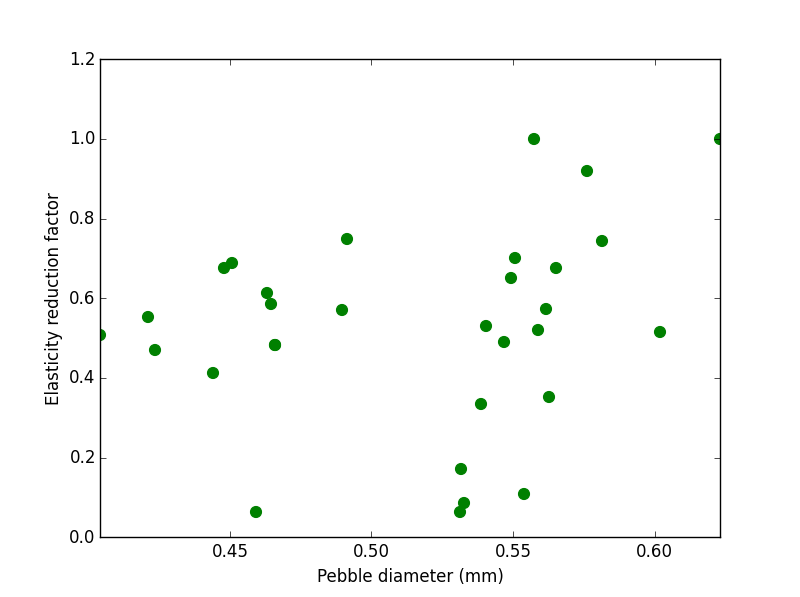
\includegraphics[width=\doubleimagewidth]{chapters/figures/fzk-kappa-dp-scatter.png}
    \caption{Scatter of $\kappa$ against pebble diameter for a batch of \lis pebbles showing almost no relationship between apparent stiffness and diameter.}
    \label{fig:fzk-kappa-dp-scatter}
\end{figure}

\begin{figure}
        \centering
        \begin{subfigure}[b]{\doubleimagewidth}
                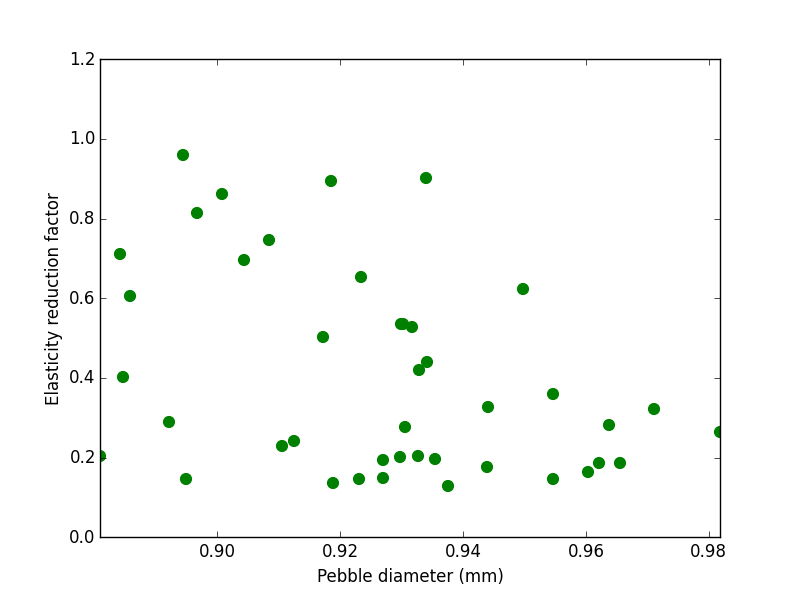
\includegraphics[width=\textwidth]{chapters/figures/nfri-1mm-kappa-dp-scatter.png}
                \caption{$\bar{d}_p = 1$ mm}
                \label{fig:nfri-1mm-kappa-dp-scatter}
        \end{subfigure}
        ~
        \begin{subfigure}[b]{\doubleimagewidth}
                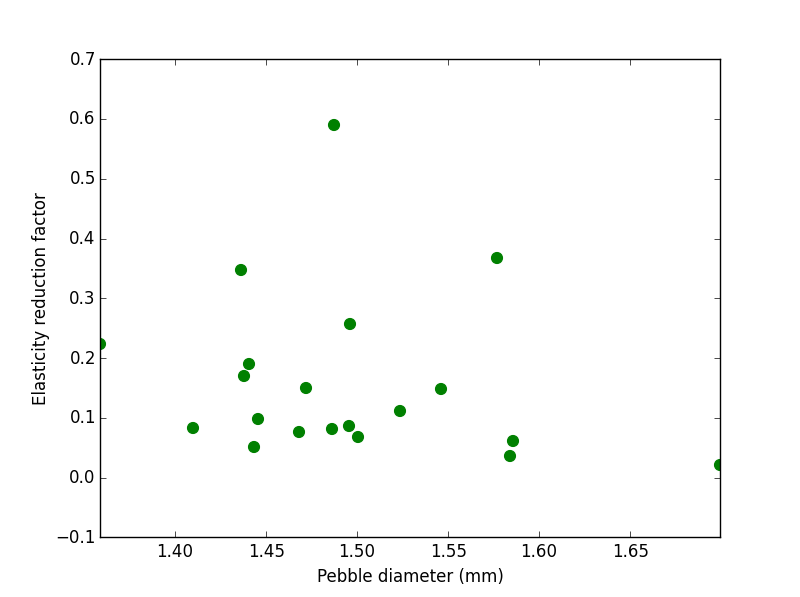
\includegraphics[width=\textwidth]{chapters/figures/nfri-1.5mm-kappa-dp-scatter.png}
                \caption{$\bar{d}_p = 1.5$ mm}
                \label{fig:nfri-1.5mm-kappa-dp-scatter}
        \end{subfigure}
        \caption{Scatter of $\kappa$ against pebble diameter for two batches of \lit pebbles showing almost no relationship between apparent stiffness and diameter.}\label{fig:nfri-kappa-dp-scatter}
\end{figure}






The Young's modulus and Poisson ratio of the test stand are known values that do not vary between pebble experiments. Similarly, in the application of Hertz theory, we also assume the Young's modulus and Poisson ratio of the ceramic is also a known, constant value. In that case, for any given pebble diameter, the term inside $[\,]$ is composed of entirely of constants for any given pebble; there is therefore a single force-travel response possible based on $s$. Using the material properties given in Ref.~\cite{Gierszewski1998} for \lit, we plot a set of parametric curves based on diameter over a range of travel. The properties we have used for the nickel-alloy anvil of our test stand and \lit are given in Table~\ref{tab:hertz-dp-study-props}. The curves are given in Fig.~\ref{fig:hertz-dp-dependence}.

\begin {table}[htp] %
\caption{Material properties used for \lit and nickel-alloy platen}
\label {tab:hertz-dp-study-props} \centering %
\begin {tabular}{ cccccc }
\toprule %
$E_\text{peb}$      &     $\nu_\text{peb}$  &   $E_\text{stand}$        &     $\nu_\text{stand}$    \\
(GPa)           &                   &   (GPa)               &                   \\\toprule
126             &   0.24                &   220                 &   0.27                \\\bottomrule
\end{tabular}
\end{table}

Figure~\ref{fig:hertz-dp-dependence} shows that, for a given pebble diameter, there is a  is strictly obeying Hertz theory, there is only a single force-displacement curve it can follow. However, when experiments are performed on single pebbles of \lis we see responses in the dashed lines of Fig.~\ref{fig:fzk-exp-colormap}. Similarly for the dashed lines of \lit in Fig.~\ref{fig:nfri-exp-curves}.

Contrary to the diameter dependence seen in Fig.~\ref{fig:hertz-dp-dependence}, the curves of Figs.~\ref{fig:fzk-exp-colormap},~\ref{fig:nfri-exp-curves} do not demonstrate any relationship between diameter and force. For comparison, the solid lines on the figures for each ceramic show the predicted Hertzian response as calculated by Eq.~\ref{eq:contact-force} based on the measured diameter of each pebble. For both the \lis and \lit pebbles, there are very few pebbles that show a measured force-travel response that is similar to the Hertzian prediction based on the material properties reported in literature. We conclude that variations in pebble diameter can not alone account for the variations in the force curves measured for the pebbles in our experiments. %The most reasonable source for variation is in the Young's modulus of pebbles in a batch. Such a conclusion is important for implementation of Hertz theory in DEM algorithms.

We hypothesize that variation in measured curves is due to each pebble having Young's modulii that diverge from the values measured from sintered blocks as reported in literature. Therefore each pebble displays a different apparent Young's modulus in the single pebble experiments. The apparent Young's modulus of each pebble is rooted in the manufacture of the pebbles which yields pebbles with slightly different internal structures. The differences in internal structure then cause the pebble to behave with different stiffnesses than the value expected from measurements of sintered pellets of lithium ceramics. In fact, the solid lines in Figs.~\ref{fig:fzk-exp-colormap},~\ref{fig:nfri-exp-curves}, as calculated from the measurements of sintered pellets, appear to be an upper limit to the pebbles. Therefore we consider pebbles will emerge with values less than the value from literature, $E_\text{lit}$ by some factor. To quantify the deviation of each pebble's $E_\text{peb}$ from the sintered pellet, we introduce a $\kappa$ factor, which we define as the elasticity reduction factor:

\begin{equation}
\kappa = \frac{E_\text{peb}}{E_\text{lit}}
\end{equation}
where
\[
\kappa \in [0,1]
\]

If each pebble has a unique $\kappa$ value, it would quantify the spread in elastic responses seen in the experiments. We find the value by assuming that the pebbles are, in fact, behaving in a Hertzian manner and we can fit the Hertzian to our experimental measurements. This allows us to back-out a $\kappa$ value, or in other words the unique $E_\text{peb}$ of that pebble. We take the sintered pebble value of Young's modulus for \lis to be $E_\text{lit} = \si{90 GPa}$ and the value for \lit to be $E_\text{lit}= \si{124 GPa}$. Then we iterate over all values of $k\in[0,1]$ and compare the Hertzian response to that pebbles force-displacement curve. At each iteration, the L2-norm of the difference between Hertzian and experimental curves is used as the `error'. The L2 norm, $A$ for a given array, $a$ is 

\begin{equation}
||A||_F = \left[\sum_{i,j}\textrm{abs}(a_{i,j})^2\right]^{1/2}
\end{equation}

This is a convenient way to compare the error at every point along the force-displacement curves. When the error is minimized, the elasticity reduction value corresponding the minimum is recorded for that pebble. In The Hertzian curves (in black) for each pebble are plotted in green against the experimental curves in Figs.~\ref{fig:fzk-exp-hertz},~\ref{fig:nfri-exp-hertz}. 



Many of the curves for \lis in Fig.~\ref{fig:fzk-exp-hertz} seem to be fit well with a Hertzian curve with modified Young's modulus. The value of Young's modulus found for each pebble is plotted in Fig.~\ref{fig:fzk-E-plot}. The Young's modulus of pebble numbers 0 to 4 are the very soft pebbles seen with very low forces on Fig.~\ref{fig:fzk-exp-hertz}. The majority of pebbles, however, behave with a Young's modulus between 30 and 70 \si{GPa}. On the upper end, a few pebbles acted very similar to their sintered pellet counterpart with approximate value of \si{90 GPa}. 

The two batches of \lit pebbles we analyzed (Fig.~\ref{fig:nfri-exp-hertz}) are similarly fit well to different Hertzian curves. The apparent Young's modulii of the \lit pebbles are given in Fig.~\ref{fig:nfri-E-plot}. These \lit pebbles have a large distribution of stiffness, from between 20 to 120~GPa for the 1~mm pebbles and roughly 2 to 80~GPa for the 1.5~mm pebbles.


A histogram of the $\kappa$ factor for this batch of \lis pebbles is given in Fig.~\ref{fig:fzk-kappa-hist}. For the \lis pebbles, the histogram resembles a normal distribution but for the large spike in pebbles with very small $\kappa$. When we look back to the force-travel plots of Fig.~\ref{fig:fzk-exp-colormap}, the four softest pebbles show similar trends of long, relatively flat responses to travel before reaching a point where there is a sharp increase in the $F-s$ slope. In the experiments, the flat sections of the curve occurred when the pebbles in the anvil were not perfectly spherical and rotated slightly under the application of a load. Once the pebbles rotated into a flat spot that could take a normal load without any angular moment, the force increased quickly under further travel. In light of this, it is unreasonable to consider their $\kappa$ values as representing their true stiffness. Neglecting the four outliers in the histogram of Fig.~\ref{fig:fzk-kappa-hist}, we are then left with a distribution much more closely resembling a normal probability distribution.

The histograms for the two batches of \lit are given in Fig.~\ref{fig:nfri-kappa-hist}. The distributions for both batches of \lit pebbles more closely resemble Snedecor's F distribution with many pebbles behaving with a very small $\kappa$.

In Figs.~\ref{fig:fzk-kappa-dp-scatter} and~\ref{fig:nfri-kappa-dp-scatter} we see scatter plots of the pebble diameters and $\kappa$ values for the different batches of lithium ceramic pebbles. A Pearson Correlation value was calculated for each of the batches to find a relationship between diameter and $\kappa$. For the \lis pebbles, we find $R = 0.198$ which is a weak positive correlation. For the \lit pebbles we have $R = -0.385$ for $\bar{d}_p = 1$~mm and $R = -0.201$ for $\bar{d}_p = 1.5$~mm. Both of these are weakly negatively correlated. 

The implications of these results are that the Young's modulus traditionally used in DEM simulations for ceramic pebble beds in solid breeders is incorrect. In \cref{sec:dem-studies-youngs-modulus}, we will introduce $\kappa$, the elasticity reduction factor, into our DEM simulations. Numerical recreations of the probability distribution curves will be used to apply $\kappa$ to pebbles in the ensemble. From the weak correlations between diameter and $\kappa$, we are free to ignore any diameter dependence when assigning $\kappa$ values in the DEM framework. In the module where we assign Young's modulus to the particles in the ensemble will apply the distribution in a random fashion.

\FloatBarrier
\subsection{Translating Experimental Results to Pebble Bed Interactions}\label{sec:theoryStrainEnergy}

It is impractical, if not impossible, to accurately measure the contact forces between all the pebbles in a densely-packed, three-dimensional ensemble. In investigating the probability of pebbles becoming damaged (i.e. crushed or cracked) in a packed bed, we therefore rely on the combined information gained from indirect measurements of the entire pebble bed, crush experiments of individual pebbles, and the predictive capabilities of DEM simulations. In this study we look at the results of individual pebble crush experiments and create a metric to link the data to the contact forces measured in DEM to help predict when pebbles in the ensemble will become damaged.

\subsubsection{Experimental Measurements of Strain Energy}
\begin{figure}[!t]
\centering
    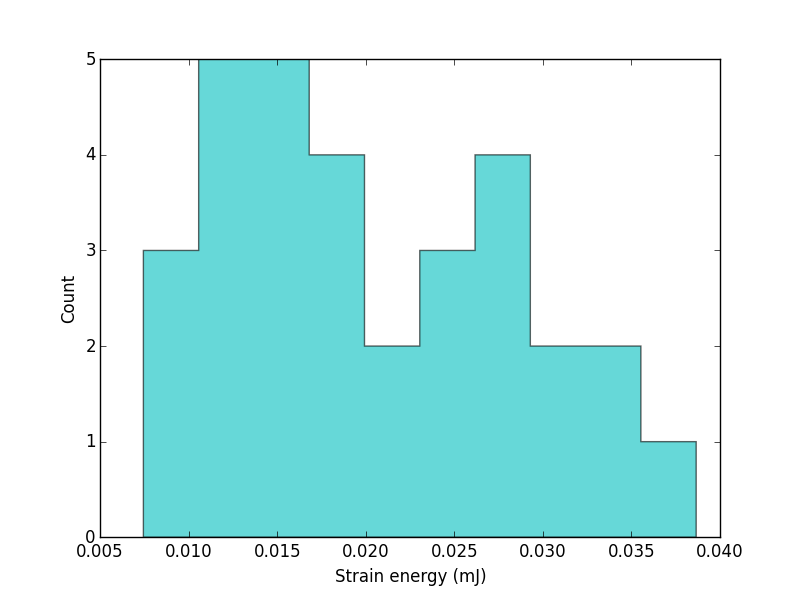
\includegraphics[width=\doubleimagewidth]{chapters/figures/fzk-w-histogram.png}
    \caption{Histogram of the absorbed strain energy at the moment of crushing for \lis pebbles as measured in single pebble crush experiments.}
    \label{fig:fzk-w-hist}
\end{figure}

\begin{figure}
        \centering
        \begin{subfigure}[b]{\doubleimagewidth}
                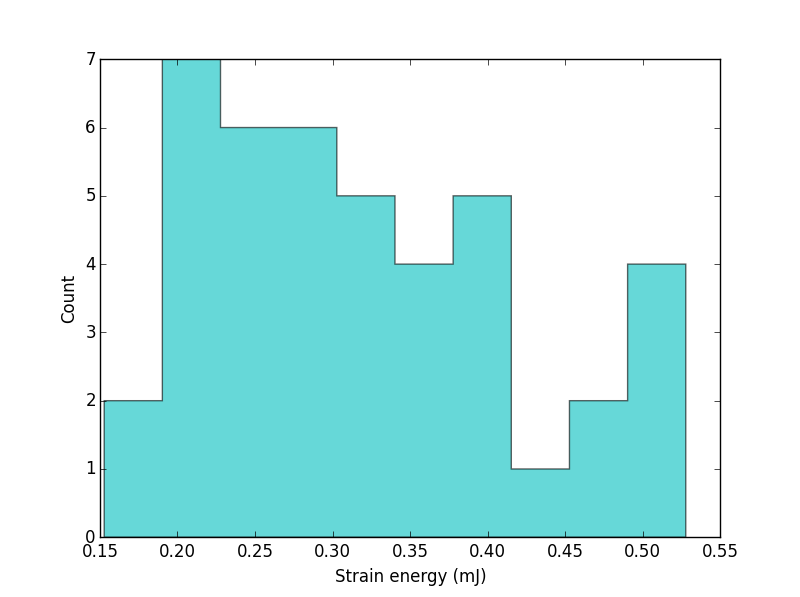
\includegraphics[width=\textwidth]{chapters/figures/nfri-1mm-w-histogram.png}
                \caption{$\bar{d}_p = 1$ mm}
                \label{fig:nfri-1-w-hist}
        \end{subfigure}
        ~
        \begin{subfigure}[b]{\doubleimagewidth}
                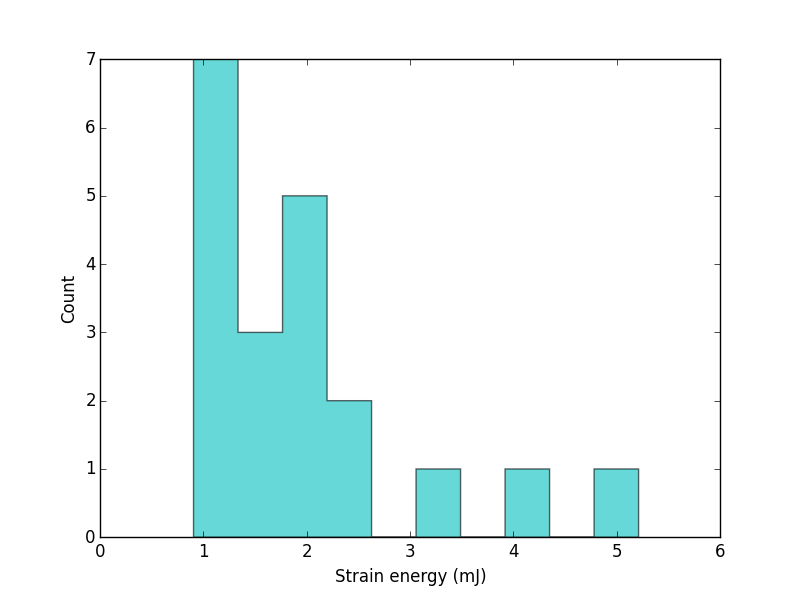
\includegraphics[width=\textwidth]{chapters/figures/nfri-1.5mm-w-histogram.png}
                \caption{$\bar{d}_p = 1.5$ mm}
                \label{fig:nfri-1.5-w-hist}
        \end{subfigure}
        \caption{Histogram of the absorbed strain energy at the moment of crushing for \lit pebbles as measured in single pebble crush experiments.}\label{fig:nfri-w-hist}
\end{figure}

The normal force between two elastic objects is a function of the material properties of the interacting objects (see Eq.~\ref{eq:hertz-normal-force}). We cannot, therefore, directly compare the forces between pebble-test stand with pebble-pebble in an ensemble. An approached used by some solid breeder researchers is to relate the absorbed strain energy of the pebble\cite{Zhao2013,Annabattula2012a}. We integrate the Hertzian force along the overlap to find the strain energy, $W_\epsilon$, of that contact. 

\begin{equation}\label{eq:strain-energy-integral}
	W_\epsilon = \int_0^{\delta_c}\!F_n(\delta')\,\mathrm{d}\delta'
\end{equation}
where the upper limit of the integration is the critical overlap $\delta_c$. Inserting Eq.~\ref{eq:hertz-normal-force} into Eq.~\ref{eq:strain-energy-integral},
\begin{align}
	W_\epsilon& = \int_0^{\delta_c}\!  \frac{4}{3}E^*\sqrt{R^*}\,\delta'^{3/2} \,\mathrm{d}\delta' \\
	%W_\epsilon & = \frac{4}{3}E^*\sqrt{R^*} \left[\frac{2}{5}\,{\delta_c}^{5/2}\right] \\
	W_\epsilon & = \frac{8}{15}E^*\sqrt{R^*}\, {\delta_c}^{5/2}
\end{align}

We will call the strain energy of the pebble compressed between platens as the lab strain energy, $W_{\epsilon,L}$. In pebble crushing experiments, we record the strain energy absorbed up to the point of crushing, the data for \lis and \lit pebbles are given in Figs.~\ref{fig:fzk-w-hist} and~\ref{fig:nfri-w-hist}, respectively. Then the strain energy of two particles in contact will be $W_{\epsilon,B}$. The assumption we make is that, if each contact interaction is integrated to the proper critical overlap, the strain energies will be equal at that contact.

\begin{equation}
	W_{\epsilon,L} = W_{\epsilon,B} = \frac{8}{15}E_B^*\sqrt{R_B^*}\, {\delta_{c,B}}^{5/2}
\end{equation}

We solve for the interacting pebble bed overlap as a function of the lab strain energy as

\begin{equation}
	\delta_{c,B} = \left[\frac{15W_{\epsilon,L}}{8E_B^*\sqrt{R_B^*}}\right]^{2/5}
\end{equation}

This overlap can be reinserted to the Hertz force of Eq.~\ref{eq:hertz-normal-force} to find the critical force (crush force) of the interacting particles as a function of the critical strain energy of the lab. Doing this, we find,
\begin{equation}\label{eq:peb_hertz}
	F_{c,B} = C{E_B^*}^{2/5}{R_B^*}^{1/5}W_{\epsilon,L}^{3/5}
\end{equation}
where $C = \frac{4}{3}\left(\frac{15}{8}\right)^{3/5}$.

Equation~\ref{eq:peb_hertz} is a generic translation between lab materials and packed bed materials. We will use the equation as the basis for our pebble crushing prediction in DEM simulations.





% FROM SOFT PAPER
\subsubsection{Calculating Critical Strain Energy}
With the rise of micro-mechanical tools and computing power, attempting to predict when ceramic pebbles will crush in an ensemble, based on inter-particle contact forces, has received considerable attention. In this section we will review literature studying granular crushing.

Probability and statistics were applied to the study of packed beds of brittle grains by Marketos and Bolton\cite{Marketos2007}. The fundamental assumption in their predictive method was the independence of crushing events. They used their model to predict the initiation of crushing as well as the evolution of the packing after crushing. They created somewhat arbitrary probability distributions of the strength of their granular particles,
\begin{equation}
	h(\Phi) = \frac{0.0395}{\sqrt{\Phi}}
\end{equation}
where $\Phi$ is a characteristic strength parameter falling between 160 and 640~N. The form of their distribution was based on single crushing tests on quartz particles from Nakata\etal.

A common alternative distribution is to use a form first proposed by Weibull for a material under uniform stress\cite{Kwok2013,Zhao2011,nakata1999probabilistic,Zhao2013,Pitchumani2004}. The form, as written by Zhao\etal~is,
\begin{equation}
	P_s = 1 - \exp\left[-\left(\frac{W_c}{W_\text{mat}}\right)^m\right]
\end{equation}
where $W_c$ is the energy absorbed by the pebble and $W_\text{mat}$ and $m$ characterize the material. An important note is how to calculate the critical strain energy for the pebble. Refs.~\cite{Marketos2007} and \cite{Zhao2011} note the necessity to consider the coordination number dependence on total strain energy. In other words, the total strain energy is the cumulative total of strain energy at every contact. Zhao\etal~give strain as
\begin{equation}
	W_c = \sum_{i=1}^{Z_i}\left(\frac{9}{80 R_{ij}^*}\right)^{1/3} \left(\frac{1}{E_{ij}^*}\right)^{2/3} F_{n,ij}^{5/3}
\end{equation}
where $Z$ is the coordination number of pebble $i$. 

However, Russell\etal, analyzed ideal granular assemblies for which they could find analytical solutions to stress distributions inside of pebbles.\cite{Russell2009} In their work, failure of a granular particle initiates at the location of maximum of the stress invariant ratios. In the contact of elastic spheres, the stress fields near the contact areas are highly localized. Because of the highly localized effects, Russell\etal~find that in granular assemblies the contributions to failure initiation are not additive. They discovered that the initiation of failure is always located adjacent to the largest force irrespective of the material properties or geometric size of the pebbles in an ensemble. Russell\etal\cite{Russell2009} conclude: the largest contact force acting upon a particle is the primary agent driving the damage of the individual. Based upon the failure criterion developed for brittle materials, crushing of an individual does not directly depend upon the presence or magnitude of any lesser contact forces acting on the particle or the material properties of the particle. Although their results were obtained for idealized assemblies, the results are generally true for any situation where multiple contact forces are present.

\begin{figure}[!t]
\centering
    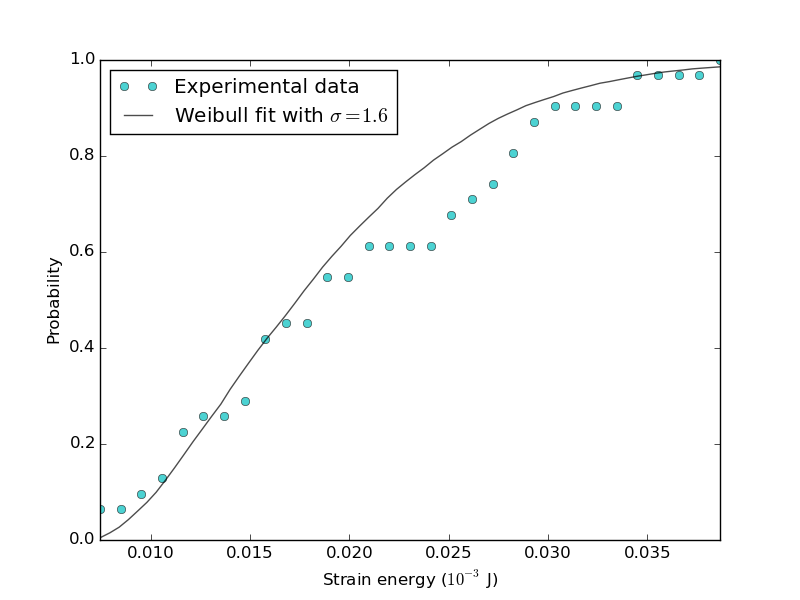
\includegraphics[width=\doubleimagewidth]{chapters/figures/fzk-w-cdf-fit.png}
    \caption{Fitting the strain energy with a Weibull distribution with shape parameter specific for the \lis pebbles.}
    \label{fig:fzk-w-cdf}
\end{figure}

\begin{figure}
        \centering
        \begin{subfigure}[b]{\doubleimagewidth}
                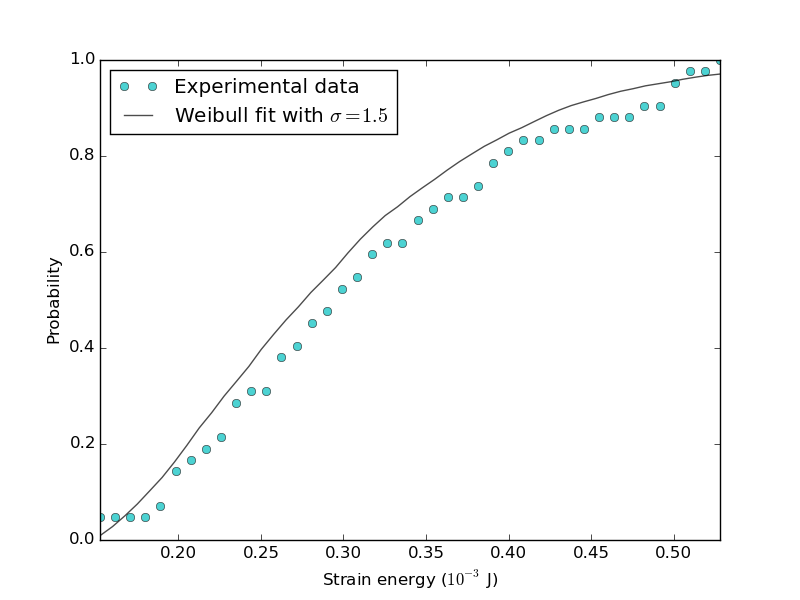
\includegraphics[width=\textwidth]{chapters/figures/nfri-1mm-w-cdf-fit.png}
                \caption{$\bar{d}_p = 1$ mm}
                \label{fig:nfri-1-w-cdf}
        \end{subfigure}
        ~
        \begin{subfigure}[b]{\doubleimagewidth}
                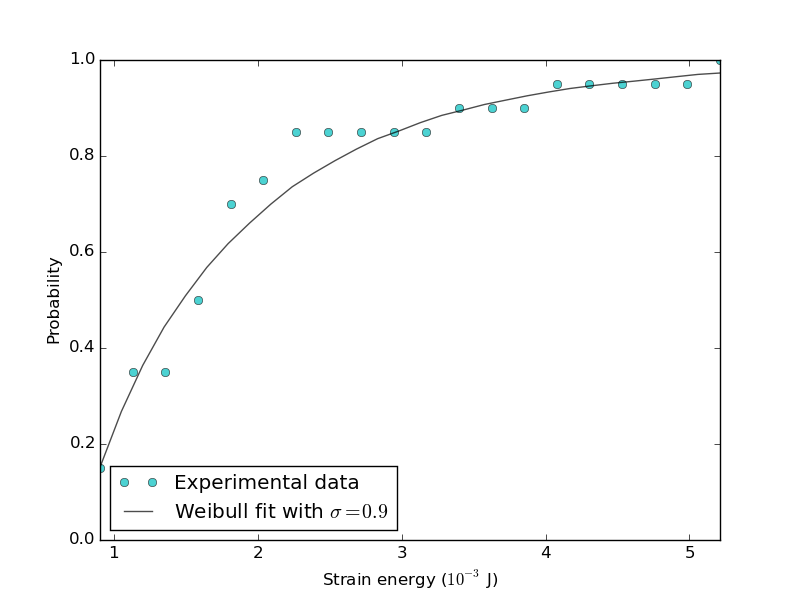
\includegraphics[width=\textwidth]{chapters/figures/nfri-1.5mm-w-cdf-fit.png}
                \caption{$\bar{d}_p = 1.5$ mm}
                \label{fig:nfri-1.5-w-cdf}
        \end{subfigure}
        \caption{Fitting the strain energy with a Weibull distribution with shape parameter specific for the two batches of \lit pebbles.}\label{fig:nfri-w-cdf}
\end{figure}

Based on the compelling arguments of Russell\etal, we will define our critical force as the maximum contact force on the pebble in our assembly,
\begin{equation}
	F_{c} = \max F_{n,ij}
\end{equation}

Then we can say a pebble is crushed when the force on the pebble in the bed is greater than the critical bed force defined from Eq.~\ref{eq:peb_hertz},

\begin{equation}\label{eq:crush-predict}
  F_{c} > F_{c,B} = \frac{4}{3}\left(\frac{15}{8}\right)^{3/5}{E_B^*}^{2/5}{R_B^*}^{1/5}W_{\epsilon,L}^{3/5}
\end{equation}

In the implementation into DEM, the probabilistic features appear naturally in this formulation from the measured probability distribution of $W_{\epsilon,L}$. In the experiments on crushing individual pebbles, the critical strain energy is measured strain energy at the point of crushing. This value follows a probability distribution and therefore imparts a distribution shape to the $F_{c,B}$ prediction. Cumulative distribution functions are generated for the strain energy data (see Figs.~\ref{fig:nfri-w-hist} and~\ref{fig:nfri-w-hist}). From that data, we fit Weibull distribution curves, of the form
\begin{equation}
	\Xi = \lambda\left[-\ln(W_\epsilon)\right]^{1/\sigma}
\end{equation}
where the shape parameter, $\sigma$, is fit to the specific curve of each set of experimental data and the second parameter, $\lambda$ is
\[
\lambda = \bar{W}_\epsilon - \min W_\epsilon
\]

In Figs.~\ref{fig:fzk-w-cdf} and~\ref{fig:nfri-w-cdf} we show the experimental data and the Weibull fits specific to the ceramic material and batch. The Weibull distribution functions will be used again when we generate strength parameters to assign to pebbles in the discrete element simulations of pebble crushing, addressed in \cref{sec:failure-study}.
\section{Linking interactions with strain energy}\label{theoryStrainEnergy}
Hertz theory is applicable to any two contacting elastic objects. In practice, we cannot probe the contacts of small particles and rely on experiments where we press pebbles between flat platens. Here we will develop a theory for connecting the results of the experiments with the interaction of two spherical objects.

To relate the situation in the lab to two particles, we first integrate the Hertzian force along the overlap to find the strain energy, $W_\epsilon$, of that contact. 

\begin{equation}
	W_\epsilon = \int_0^{\delta_c}\!F_n(\delta')\,\mathrm{d}\delta'
\end{equation}

where the upper limit of the integration is the critical overlap $\delta_c$ (the meaning of this value will be explained in detail later). With the force defined from Eq.~\ref{eq:hertzForce}, this is straightforward to integrate.

\begin{align}
	W_\epsilon& = \int_0^{\delta_c}\!  \frac{4}{3}E^*\sqrt{R^*}\,\delta'^{3/2} \,\mathrm{d}\delta' \\
	%W_\epsilon & = \frac{4}{3}E^*\sqrt{R^*} \left[\frac{2}{5}\,{\delta_c}^{5/2}\right] \\
	W_\epsilon & = \frac{8}{15}E^*\sqrt{R^*}\, {\delta_c}^{5/2}
\end{align}

We will call the strain energy of the pebble compressed between platens as the lab strain energy, $W_{\epsilon,L}$. The strain energy of two particles in contact will be $W_{\epsilon,B}$. The assumption we make is that, if each interaction is integrated to the proper critical overlap, the strain energies will be equal at that point.

\begin{equation}
	W_{\epsilon,L} = W_{\epsilon,B} = \frac{8}{15}E_B^*\sqrt{R_B^*}\, {\delta_{c,B}}^{5/2}
\end{equation}

We solve for the interacting particle overlap as a function of the lab strain energy as

\begin{equation}
	\delta_{c,B} = \left[\frac{15W_{\epsilon,L}}{8E_B^*\sqrt{R_B^*}}\right]^{2/5}
\end{equation}

This overlap can be reinserted to Eq.~\ref{eq:hertzForce} to find the critical force of the interacting particles as a function of the critical strain energy of the lab. Doing this, we find:

\begin{equation}\label{eq:peb_hertz}
	F_{c,B} = C{E_B^*}^{2/5}{R_B^*}^{1/5}W_{\epsilon,L}^{3/5}
\end{equation}

where $C = \frac{4}{3}\left(\frac{15}{8}\right)^{3/5}$.

In this analysis we have referred to a `lab' and `particle' for the two situations. In fact, the result is more general and can be used to relate any two scenarios. The only requirement is that both conditions adhere to the assumptions of Hertz theory. The ramifications of this relationship will be explored in more detail in \cref{analysisExp}.





% FROM SOFT PAPER
\subsection{Pebble crushing predictions}
Along with proper material properties, we present a relationship to translate between the experimental data of crush force to a value that can be applied to DEM simulations. We relate crush force experimental data to predictions of crushing pebbles in an ensemble with:

\begin{equation}\label{eq:crush-predict}
  F_{c,B} = \frac{4}{3} \left(\frac{15}{8}\right)^{2/5}\left(R_B^* \right)^{1/5}\left( W_{\epsilon,L} \right)^{3/5}
\end{equation}

where $W_{\epsilon,L}$ is measured strain energy at the point of crushing from the experiment. This value follows a probability distribution and therefore imparts a distribution shape to the $F_{c,B}$ prediction. At the peak load of 6 MPa we use the above prediction to determine how many pebbles would be cracking at this state of external pressure



\appendix
\chapter{Sphere with heat generation}\label{sec:analytic-sphere-details}

We solve for the temperature distribution inside a single sphere of constant thermal conductivity with constant heat generation with a convective heat transfer boundary condition. To simplify to homogeneous boundary conditions, the temperature we solve for will be in reference to the fluid temperature, $\mathbb{T} = T-T_f$. 

The energy equation in spherical coordinates with axial symmetry is,

\begin{equation}
    \frac{1}{r}\frac{\partial^2}{\partial r^2}(r\mathbb{T}) + \frac{g}{k} = \frac{1}{\alpha}\frac{\partial \mathbb{T}}{\partial t}
\end{equation}

which is subject to the boundary conditions of a constant heat transfer coefficient at the surface, $h$,

\begin{equation}
    \left[\frac{\partial \mathbb{T}}{\partial r} + \frac{h}{k}\mathbb{T}\right]_{r=b} = 0
\end{equation}

and an axisymmetry at the center,

\begin{equation}
    \left[\frac{\partial \mathbb{T}}{\partial r}\right]_{r=0} = 0
\end{equation}

The sphere will be at an isothermal initial temperature,

\begin{equation}
    \mathbb{T}(r,0) = \mathbb{T}_0
\end{equation}





\section{Transformations}

We first transform the system into the nondimensional forms as defined in \S\ref{sec:ht-jeffreson-correction},

\begin{align*}
    \theta &= \frac{\mathbb{T}}{\mathbb{T}_0}\\
    \rho & = \frac{r}{b}\\
    \tau & = \frac{t}{b^2/\alpha}
\end{align*}

The energy equation is then,
\begin{equation}
    \frac{1}{\rho}\frac{\partial^2}{\partial \rho^2}(\rho\theta) + G = \frac{\partial\theta}{\partial \tau}
\end{equation}

where $G = \frac{gb^2}{k\mathbb{T}_0}$

The next transformation will be to introduce $U(\rho,\tau) = \rho\theta(\rho,\tau)$ as a transformation variable to simplify the differential equation of energy conservation. In the new variable formulation, the energy equation is,

\begin{equation}\label{eq:transformed-energy}
    \frac{\partial^2 U}{\partial \rho^2} + G\rho = \frac{\partial U}{\partial \tau}
\end{equation}

The boundary conditions are likewise transformed into,

\begin{equation}\label{eq:transformed-bc-1}
    \left[\frac{\partial U}{\partial \rho} + \left(\Bi-1\right)U\right]_{\rho = 1}= 0
\end{equation}

and

\begin{equation}\label{eq:transformed-bc-2}
    U\big|_{\rho=0} = 0
\end{equation}

with initial condition

\begin{equation}\label{eq:transformed-ic}
    U(\rho,0) = U_0 = \theta_0 r^* = r^*
\end{equation}




\section{Solution}

Because of the non-homegeneous form of the energy equation (due to the heat generation term), we will solve Eq.~\ref{eq:transformed-energy} by breaking it up into two simpler problems, 

\begin{enumerate}
\item A non-homogeneous, steady-state problem defined by $U_{ss}(r)$
\item A homogeneous, time-dependent problem defined by $U_h(r,t)$
\end{enumerate}

The steady-state distribution $U_{ss}$ is found from the solution of

\begin{equation}
    \frac{\partial^2 U_{ss}}{\partial \rho^2} + G\rho= 0
\end{equation}

subject to the same boundary condition given by Eqs.~\ref{eq:transformed-bc-1},\ref{eq:transformed-bc-2}. Separation and integration gives.

\begin{equation}
    U_{ss} = -\frac{G}{6} \rho^3 + C_1\rho + C_2
\end{equation}

Applying Eq.~\ref{eq:transformed-bc-2} directly gives $C_2 = 0$ and, with some algebra Eq.~\ref{eq:transformed-bc-1} gives, 

\begin{equation*}
    C_1 = \left(\frac{G}{6} + \frac{G}{3\Bi}\right)
\end{equation*}

valid for $\Bi > 0$. Thus the steady-state distribution of our transformed variable is

\begin{equation}\label{eq:transformed-steady-state-solution}
    U_{ss} = \left(\frac{G}{6} + \frac{G}{3\Bi}-\rho^2\right)\rho
\end{equation}

The next step is to find the homogeneous solution of 

\begin{equation}
    \frac{\partial^2 U_h}{\partial \rho^2} = \frac{\partial U_h}{\partial \tau}
\end{equation}

Again, subject to Eqs.~\ref{eq:transformed-bc-1},\ref{eq:transformed-bc-2}, but now with a modified initial condition of 

\begin{align}\label{eq:homogeneous-ic}
    U_{h,0} &= U_0 - U_{ss} \nonumber \\
    & = \left[1 - \left(\frac{G}{6} + \frac{G}{3\Bi}-\rho^2\right) \right]\rho
\end{align}

This is a standard homogeneous partial differntial equation. The solution is of the form

\begin{equation}
    U_h = R(\rho) \Gamma(\tau)
\end{equation}

The solution for $\Gamma$ is given as

\begin{equation}
    \Gamma = \exp(-\zeta^2 \tau)
\end{equation}

The space-variable function $R(\zeta,\rho)$ satisfies the following eigenvalue problem:

\begin{equation}\label{eq:eigen-function}
    \frac{\mathrm{d}^2R}{\mathrm{d}\rho^{2}} + \zeta^2 R = 0
\end{equation}

subject to 

\begin{equation}
    R_{\rho = 0} = 0
\end{equation}

and

\begin{equation}
    \left[\frac{\mathrm{d}R}{\mathrm{d}\rho} + (\Bi - 1)R\right]_{\rho=1} = 0
\end{equation}

This eigenvalue problem is a special case of the Sturm-Liouville problem. The solution for $U_h$ can be constructed from known eigenvalue solutions,

\begin{equation}\label{eq:eigen-general-solution}
    U_h(\rho,\tau) = \sum_{n=1}^\infty c_n R(\zeta_n,\rho)\exp(-\zeta^2 \tau)
\end{equation}

Application of the initial condition gives,

\begin{equation}\label{eq:eigen-initial-condition}
    F(\rho) = \sum_{n=1}^\infty c_n R(\zeta_n,\rho)
\end{equation}

where $F(\rho)$ is the initial condition defined from Eq~\ref{eq:transformed-ic}, 

\begin{equation}
    F(\rho) =\left[1 - \frac{G}{6}\left(1 + \frac{2}{\Bi}-\rho^2\right) \right]\rho
\end{equation}

The coefficients of $c_n$ can be determined by applying the operator $\int_0^1 R(\zeta_n,\rho)\,\mathrm{d}\rho$ and utilizing the orthogonality property of eigenfunctions. The coefficients are found in the form

\begin{equation}\label{eq:eigenfunction-coefficients}
    c_n = \frac{1}{N(\zeta_n)}\int_0^1 R(\zeta_n,\rho')F(\rho')\,\mathrm{d}\rho'
\end{equation}

The norm, $N$ is a function of the eigenvalues,

\begin{equation}
    N(\zeta_n) = \int_0^1 \left[R(\zeta_n,\rho)\right]^2\,\mathrm{d}\rho
\end{equation}

% Eq.~\ref{eq:eigenfunction-coefficients} is also inserted back into Eq.~\ref{eq:eigen-initial-condition},

% \begin{equation}
%     (T_0-T_f)r - \frac{g}{6k} r^3 - \frac{gb^2}{6k}\left(1 + \frac{2}{Bi}\right)r = \sum_{n=1}^\infty \frac{R(\zeta_n,r)}{N(\zeta_n)}\int_0^b R(\zeta_n,r')F(r')\,\mathrm{d}r'
% \end{equation}

The eigenfunctions for Eq.~\ref{eq:eigen-function} are

\begin{equation}
    R(\zeta_n,\rho) = \sin(\zeta_n \rho)
\end{equation}

where the eigenvalues are the root of the following transcendental equation,

\begin{equation}
    \zeta_n\cot(\zeta_n) = -H
\end{equation}

the roots of which will be found numerically. The normalization integral is then solved as

\begin{equation}
    \frac{1}{N(\zeta_n)} = 2\frac{\zeta_n^2 + H^2}{\zeta_n^2+H^2 + H}
\end{equation}

where $H = (\Bi-1)$. 

We substitute the coefficients of Eq.~\ref{eq:eigenfunction-coefficients}, they can be substituted back into Eq.~\ref{eq:eigen-general-solution} and we have a solution for the homogeneous, transient distribution,

\begin{equation}
    U_h(\rho,\tau) = \sum_{n=1}^\infty \exp(-\zeta^2 \tau) \frac{R(\zeta_n,\rho)}{N(\zeta_n)}\int_0^1 R(\zeta_n,\rho')F(\rho')\,\mathrm{d}\rho'
\end{equation}

In order to explicitly express the solution, we will first set the integral equal to a function $Z(\zeta_n)$ and evaluate as,

\begin{align}
    Z(\zeta_n) & = \int_0^1 R(\zeta_n,\rho')F(\rho')\,\mathrm{d}\rho' \nonumber\\
    & = \int_0^1\sin(\zeta_n\rho') \left[1 - \left(\frac{G}{6} + \frac{G}{3\Bi}-\rho^{'2}\right) \right]\rho'  \,\mathrm{d}\rho' \nonumber\\
    & =\left[1  - \left(\frac{G}{6} + \frac{G}{3\Bi}\right)\right]\int_0^1\sin(\zeta_n\rho')\rho' \,\mathrm{d}\rho' + \frac{G}{6}\int_0^1 \sin(\zeta_n\rho')\rho^{'3} \,\mathrm{d}\rho'
\end{align}

The two unique integrals are evaluated as

\begin{align*}
    C_n &= \int_0^1\sin(\zeta_n\rho')\rho' \,\mathrm{d}\rho'  = \frac{\sin\zeta_n-\zeta_n\cos\zeta_n}{\zeta_n^2}\\
    K_n &= \int_0^1\sin(\zeta_n\rho')\rho^{'3} \,\mathrm{d}\rho'  = \frac{3(\zeta_n^2-2)\sin\zeta_n - \zeta_n(\zeta_n^2-6)\cos\zeta_n}{\zeta_n^4}
\end{align*}

Thus our $Z$ function is

\begin{equation}
    Z(\zeta_n) = \left[1  - \left(\frac{G}{6} + \frac{G}{3\Bi}\right)\right]C_n + \frac{G}{6}K_n
\end{equation}

The homogeneous solution is then written in a compact form as,

\begin{equation}\label{eq:transformed-transient-solution}
    U_h(\rho,\tau) = \sum_{n=1}^\infty \exp(-\zeta^2 \tau) \sin(\zeta_n \rho) \frac{Z(\zeta_n)}{N(\zeta_n)} 
\end{equation}

The complete solution is then a superposition of Eq.~\ref{eq:transformed-steady-state-solution} and Eq.~\ref{eq:transformed-transient-solution},

\begin{equation}
    U(\rho,\tau) = \left(\frac{G}{6} + \frac{G}{3\Bi}-\rho^2\right)\rho  +   \sum_{n=1}^\infty \exp(-\zeta^2 \tau) \sin(\zeta_n \rho) \frac{Z(\zeta_n)}{N(\zeta_n)} 
\end{equation}

We now transform back to our dimensionless temperature,

\begin{equation}\label{eq:temperature-solution}
    \theta(\rho,\tau) = \left(\frac{G}{6} + \frac{G}{3\Bi}-\rho^2\right)  +   \sum_{n=1}^\infty \exp(-\zeta^2 \tau) \frac{\sin(\zeta_n \rho)}{\rho} \frac{Z(\zeta_n)}{N(\zeta_n)}  
\end{equation}


\section{Energy}

We will want to compare the solution of Eq.~\ref{eq:temperature-solution} to that of a sphere with the lumped capacitance assumption. To facilitate comparison, we look to a measure of the energy of the sphere (with radial dependence removed via integration of Eq.~\ref{eq:temperature-solution}). The energy will be nondimensionalized as,

\begin{equation}
    E^*(\tau)=\frac{E(\tau)}{E_0}
\end{equation}

where $E_0$ is the initial energy of the sphere,

\begin{equation}
    E_0=\rho_rC_rV\mathbb{T}_0
\end{equation}

Thus the nondimensional energy of the sphere at a given time, $\tau$ is

\begin{align}
    E^*(\tau) &=\int\frac{\rho_rC_r\mathbb{T}(\rho,\tau)\mathrm{d}V}{\rho_rC_rV\mathbb{T}_0} \nonumber\\
    E^*(\tau) &=\frac{1}{V}\int \theta(\rho,\tau) \,\mathrm{d}V
\end{align}


For a circle in spherical coordinates:

\begin{equation}
    \mathrm{d}V=r^2\sin(\phi)\mathrm{d}r\mathrm{d}\phi \mathrm{d}\theta
\end{equation}

For our sphere, this becomes:

\begin{equation}
    \mathrm{d}V=4\pi b^3 \rho^{2}\mathrm{d}\rho = 3V \rho^{2}\mathrm{d}\rho
\end{equation}

The integral for dimensionless energy of our sphere is then,

\begin{equation}
    E=3\int_0^1  \left[ \frac{G}{6}\left(1 + \frac{2}{\Bi}-\rho^2\right)  +   \sum_{n=1}^\infty \exp(-\zeta^2 \tau) \frac{\sin(\zeta_n \rho)}{\rho} \frac{Z(\zeta_n)}{N(\zeta_n)}  \right] \rho^{2}\,\mathrm{d}\rho
\end{equation}

This ultimately reduces to,

% \begin{equation}
%     E^*_{t.g.}=    3\left\{ \frac{G}{6}\left(1+\frac{2}{Bi}\right)\int_0^1 \rho^{2}\,\mathrm{d}\rho - \frac{G}{6}\int_0^1 \rho^{4}\,\mathrm{d}\rho  +   \sum_{n=1}^\infty \exp(-\zeta^2 \tau) \frac{Z(\zeta_n)}{N(\zeta_n)} \int_0^1 \sin(\zeta_n \rho) \rho\,\mathrm{d}\rho\right\}
% \end{equation}

% The first two integrals are simply $\frac{1}{3}$ and $\frac{1}{5}$, respectively. We recognize the last integral as one which we solved previously. Thus,

\begin{equation}
\label{eq:energy-exact}
    E^*=\left(\frac{G}{15}+\frac{G}{3\Bi}\right)+3\sum_{n=1}^\infty \exp(-\zeta^2 \tau) \frac{Z(\zeta_n)}{N(\zeta_n)} C_n(\zeta_n)
\end{equation}



%\input{Appendix6.tex}


\bibliographystyle{ieee}
\bibliography{library}
\end{document}
